% \documentclass[10pt]{article}
\documentclass[a4paper,10pt,twocolumn]{article}
\setlength\columnsep{6mm}

% For omitting images during build from CLI
\ifdefined\noimage
    \usepackage[demo]{graphicx}
\else
    \usepackage{graphicx}
\fi

\usepackage[english]{babel}
\usepackage[stretch=10, shrink=11]{microtype}
% \usepackage[a4paper]{geometry}
\usepackage[a4paper, total={6.5in, 9in}]{geometry}
\usepackage[hyphens]{url}
\usepackage{caption}
\usepackage{subcaption}
\usepackage{amsmath}
\usepackage{multirow}
\usepackage{xcolor}
\usepackage{hyperref}
\usepackage{float}
\usepackage[linesnumbered,lined,commentsnumbered]{algorithm2e}
\usepackage{enumitem}
\usepackage{dblfloatfix}
\usepackage{texlogos}
\usepackage{chngpage}

% \usepackage[backend=bibtex]{biblatex}
% \bibliography{thesis.bib}

% Tighter vspace in enumerate/itemize
% \setlist{noitemsep,topsep=0pt,parsep=0pt,partopsep=0pt}

\hypersetup{  % Prevents colored boxes around \cite and \ref
    allbordercolors = {white}
}

\newcommand{\note}[2]{#1${}_{#2}$}
\newcommand{\notesharp}[2]{#1${}_{#2}^{\sharp}$}
\newcommand{\noteflat}[2]{#1${}_{#2}^{\flat}$}

\newcommand{\floor}[1]{\left \lfloor #1 \right \rfloor}
\newcommand{\ceil}[1]{\left \lceil #1 \right \rceil}
\newcommand{\round}[1]{\left \lfloor #1 \right \rceil}

\let\oldnl\nl% Store \nl in \oldnl
\newcommand{\nonl}{\renewcommand{\nl}{\let\nl\oldnl}}


\title{\textbf{Real-time monophonic pitch estimation for guitar driven sound synthesis}}
% \title{\textbf{Real-time monophonic guitar pitch estimation\\using 12 tuned concurrent Fourier transforms}}
% \title{\textbf{Fourier transform based real-time pitch estimation}\\Assessing the limits of Fourier transform based real-time pitch estimation and construction of a pitch estimation framework}
\author{Luc de Jonckheere}
% \date{}

\begin{document}
\selectlanguage{english}

\ifdefined\notitle
    %
\else
    \maketitle
\fi


\section*{Abstract}
% \textcolor{red}{Note that even though we focus on guitar pitch estimation, the methods described in this thesis are general to all instruments and even singing. The only guitar specific thing is the parameter optimization. We focus on guitar as it is not easily replaced by a MIDI variant as is possible with instruments such as a piano.}
In this thesis, we research real-time monophonic pitch estimation. Specifically, we focus on Fourier transform based methods. The limiting factor with these methods is the trade-off between latency and spectral resolution. In order to discern the two lowest notes of a typical guitar (\note{E}{2} and \note{F}{2}), we need a frequency resolution of 4.9 Hz, equating to a latency of 200 milliseconds. This significantly exceeds our real-time constraint of 20 milliseconds. Through interpolation, we were able to reduce the latency to 43 milliseconds.

In order to push latency to a minimum, we developed a pitch estimation framework called Digistring. Digistring provides a wide range of pitch estimation tools; from efficient implementations of common pitch estimation functions to extensive feedback and experimentation tools. Furthermore, Digistring can synthesize audio and drive existing MIDI synthesizers in real-time based on the pitch estimations of the incoming audio.
\ifdefined\notitle
    \vfill
    \pagebreak
    \!
    \pagebreak
\fi

% \vfill
\ifdefined\notitle
    \onecolumn
\fi
\tableofcontents
\vfill
\ifdefined\notitle
    \pagebreak
    % \!
    % \pagebreak
    \twocolumn
\fi


\section{Introduction}
Pitch estimation, which is also referred to as $f_0$ estimation, is a subtask within the field of Automatic Music Transcription (AMT). The goal of pitch estimation is to estimate the pitch or fundamental frequency $f_0$ of a given signal. In the context of AMT, pitch estimation is used to determine which notes are played in a given signal~\cite{survey2}.

Real-time pitch estimation is a subproblem where we want to estimate the note associated with the measured pitch while the musician is playing it with minimal latency. This entails we have to use the latest received signal. In contrast to non-real-time methods, we have no knowledge of what may happen ahead of time as we cannot peak-ahead and the signal corresponding to previous notes is mostly irrelevant. This limits the methods we can use to solve this problem.

If pitch estimation can accurately be performed in real-time, it can be used to create a digital (MIDI) instrument from an acoustic instrument. This digital instrument can then be used as an input for audio synthesizers, allowing musicians to produce sounds from a wide variety of instruments. Furthermore, accurate real-time pitch estimation can be used to automatically correct detuned instruments by pitch shifting the original signal to the closest harmonious note.

%The Fourier transform is often used for pitch estimation. 
Pitch estimation often relies on the Fourier transform. The transform decomposes a signal into the frequencies that make up the signal. Predominant frequencies in the signal show up as spectral peaks in the frequency domain. These peaks are important to human perception of melody~\cite{hearing}. %The popularity of the Fourier transform in pitch estimation is likely due to its widespread use in
Other popular signal processing based methods used for pitch estimation include autocorrelation and non-negative matrix factorization. Popular data driven methods use neural networks and hidden Markov models.
% Other popular methods used for pitch estimation include autocorrelation, non-negative matrix factorization, statistical model based estimation and hidden Markov model based estimation.

Our research focuses on monophonic pitch estimation of the signal from an electric guitar. Here, we assume the signal contains at most one note. It is much easier to perform monophonic pitch estimation compared to polyphonic pitch estimation~\cite{monotopoly}, especially when using Fourier transform based methods, as fundamental limits of the Fourier transform inhibit our ability to discern two low pitched notes~\cite{nopoly}. Furthermore, hexaphonic guitar pick-ups are becoming more widespread, which allows us to view the guitar as six monophonic instruments instead of one six-way polyphonic instrument. State of the art commercial guitar synthesizer solutions also use these hexaphonic pick-ups, which indicates accurate and responsive real-time polyphonic pitch estimation is challenging.

This thesis builds upon a preliminary research project~\cite{ik}. In our research project, we found that Fourier transform based pitch estimation methods might not be well suited for real-time use due to fundamental limitations of the Fourier transform~\cite{fourierlimit}. In this work, we will further research if Fourier transform based methods are viable, as real-time pitch estimation research often relies Fourier transform based methods.

Researching pitch estimation is not accessible, as many other small problems have to be solved in order to produce a working prototype on which experiments can be performed. Furthermore, automated experimentation is challenging to implement and as a consequence, pitch estimation research often only includes some informal testing or no experiments at all. To combat these problems, we set out to create a pitch estimation framework called Digistring. Digistring provides a live execution environment for arbitrary pitch estimation algorithms, as well as tools to perform experiments on them. In addition, it provides tools such as data visualizers and estimation based sound synthesis, which aid in developing and fine-tuning pitch estimation algorithms. Digistring is available at \url{github.com/lucmans/digistring}.

% \textcolor{gray}{The goal of this thesis is to research the limits of Fourier transform based real-time pitch estimation. To correctly assess the limits, we develop a pitch estimation framework. This framework will focus on extensibility and the ability to perform automated tests. This is important, as much work in this field does not provide its associated source code. This limits the ability to build on other's work and hinders direct comparisons between different methods. Our framework can provide a common ground for the different methods and algorithms to be implemented and compared in. The framework is available at \url{www.github.com/lucmans/digistring}.}



\section{Related work}  \label{sec:related}
Much research has been performed on Fourier transform based real-time pitch estimation. All research we found relies on obtaining a high resolution frequency domain in which spectral peaks can be isolated and notes can be associated with. These methods are deemed infeasible by some due to low frequency resolution resulting from using short signal frames needed to achieve low latencies~\cite{fourierlimit}. %, however, in our research project we found that it might still be possible. The lack of resolution in the low frequencies is especially problematic when adhering to a real-time constraint, as extra short signal frames have to be used.
% This is especially problematic when adhering to a real-time constraint, as shorter signal frames cause less frequency resolution.
Some papers circumvent this problem by choosing a very high real-time constraint~\cite{sloomboi, sloomboi2}, however, this inhibits the use for real-world applications. On top of the latency from the pitch estimation algorithm, conventional operating systems also have a latency when delivering audio samples to your program due to how audio drivers work~\cite{oslatency}.

A big problem with Fourier based pitch estimation is the occurrence of overtones~\cite{oud}. Especially octaves are a problem, as the fundamental and all overtones of the higher note overlap with overtones of the lower note. This is referred to as the octave problem~\cite{octave}. Overtones are periodic in nature, as they diminishingly repeat every multiple of the fundamental frequency. As a consequence, they could also be detected using a subsequent Fourier transform~\cite{doublefourier} on the frequency domain. However, this does not solve the octave problem.

Many different transform have been researched for pitch estimation, however, the Fourier transform remains popular as it has been broadly studied and its behavior is well known~\cite{survey}. Lately, the CQT transform is gaining popularity as it may provide higher resolution in some parts of the frequency domain~\cite{cqtres} at the cost of lower computational efficiency~\cite{cqtslow}. However, the CQT transform is efficiently implemented using Fourier transforms~\cite{cqtfft}. The main problem with Fourier transform is the fundamentally low frequency resolution on short frames, thus the fundamental problem remains. An often mentioned advantage of the CQT transform is that the frequency bins can perfectly align with the notes of an instrument~\cite{cqtalign}. However, as described in Section~\ref{sec:physsound}, overtones are dissonant with respect to our notes and consequently, the CQT bins do not align with the overtones. If a note perfectly aligns with a Fourier bin, all overtones will also align. In order to cover every note, we could instead perform 12 Fourier transforms in parallel.% This difference is especially important when performing polyphonic pitch estimation.

Until recently, signal processing driven pitch estimation methods outperformed data driven methods, due to the scarcity of annotated datasets~\cite{SPICE}. Current state-of-the-art pitch estimation algorithms include CREPE~\cite{CREPE}, SPICE~\cite{SPICE} and SWIPE~\cite{SWIPE}. SWIPE is the current state-of-the-art signal processing driven pitch estimation method. It compares the input spectrum to the spectrum of sawtooth waves to estimate the pitch. CREPE uses a data driven method consisting of a deep convolutional neural network which requires supervised training. SPICE uses a self-supervised learning technique to overcome the scarcity of annotated datasets. These three methods perform similarly~\cite{SPICE}.

% \textcolor{red}{TODO: Note on problems with other research, such as no experiments, no available source code, assuming normal continuous Fourier behavior instead of DFT, downsampling}

% \textcolor{red}{TODO: Vergelijk materiaal}



\section{Preliminaries}
In order to effectively research Fourier transform based real-time pitch estimation, it is important to have a thorough understanding of how computers deal with audio and how the Fourier transform is implemented in computers. Furthermore, in order to use the output of the Fourier transform, we need to understand the characteristics of the sound generated by instruments. Moreover, in order to interpret the results of our estimated pitch and reason about the performance of the used algorithms, some music theory is necessary. Lastly, we will discuss the concept of real-time in depth, as there are multiple definitions for \textit{real-time} which often leads to incorrect use of the concept.
% In order to effectively research Fourier transform based real-time pitch estimation, it is important to have a thorough understanding of how computers deal with audio and how the Fourier transform is implemented in computers. Furthermore, we will discuss the concept of real-time in depth, as there are multiple definition for real-time which often leads to incorrect use of the concept. Moreover, in order to use the output of the Fourier transform, we need to understand the characteristics of the sound generated by instruments. Lastly, in order to interpret the results of our estimated pitch and reason about the performance of the used algorithms, some music theory is necessary.


\subsection{Audio in computers}  \label{sub:computer_audio}
Audio in computers is represented through a series of equally spaced samples. A sample is the height of the audio wave at a specific point in time. The sample rate determines the number of samples per second used for representing the audio. The sample format determines how the height of the audio wave is represented in a sample. Often used formats are 8/16/24 bit integers and 32 bit IEEE-754 floating point numbers (which we will refer to as floats). The integer samples uniformly spread the range of the waveform over the range of the integer~\cite{dspfloat}. Float samples typically take values in $[-1, 1]$. Samples with values outside this range are considered to be clipping. Because float samples have 24 bits precision (23 mantissa bits and a sign bit~\cite{ieeefloat}), 24 bit integer samples can be converted lossless to float samples. The 8 exponent bits can be used to scale the samples to a different order, which allows us to describe very soft and loud audio with less range or accuracy respectively. Float samples have many advantages over integer samples for digital signal processing, such as reduced quantization noise and increased dynamic range~\cite{dspfloat}. Because of this, we will always use float samples throughout this thesis.
% The quality of a format is often expressed as bit depth. This is fine when comparing different integer formats, as an integer uses its full bit depth to store the height of the 

% When working with audio input/output in modern operating systems such as Linux or Windows, the audio samples are gathered/retrieved from the OS's audio driver. The audio driver
When working with audio input/output in computers, a small latency is always introduced~\cite{presonus}. One part of the latency comes from the used audio hardware and is not configurable. The other part comes from the audio driver's buffers. Audio drivers work on a buffer of samples instead of single samples for computational efficiency. A full buffer of data has to be gathered from the audio input, or a full buffer has to be send to the audio output, so the first or last sample respectively is one buffer length behind. The buffer length is calculated by dividing the number of samples in the buffer by the sample rate. In order to minimize latency, the number of samples per buffer has to be minimized and the sample rate has to be maximized. As these latencies are outside of Digistring's control and can be mostly circumvented by running Digistring's algorithms on specialized hardware, we will not take them into account in this thesis.


\subsection{Fourier transform}  \label{sec:fourier}
The Fourier transform is a mathematical transform which transforms a function of time to a complex valued function of frequency. Here, the magnitude represents the amplitude and the argument represents the phase of the corresponding frequency component. The function which maps the frequencies to amplitudes is called the spectrum of the time dependent function. The Fourier transform works on continuous functions and assumes an infinite time interval. Concepts such as continuous and infinite cannot be represented by a computer. Consequently, the discrete Fourier transform (DFT) has to be used for Fourier analyses on computers. The DFT can efficiently be calculated using the fast Fourier transform (FFT) algorithm.

The DFT transforms a finite sequence of equally spaced samples, which we will refer to as a frame, into an equal number of complex values representing the amplitude and phase, which we refer to as bins. Technically, the magnitudes of the bins do not form a spectrum as they are not continuous, however, within digital signal processing it is still referred to as the spectrum of the frame. %Note that a frame may also referred to as a window.
When working with audio, the samples are real valued, and the DFT output is symmetrical. Because of this, we can discard the second half of the output. In the rest of this thesis, we will only consider the first half of the output. Each bin corresponds to a specific frequency. All other frequencies are spread out over multiple bins. This is called spectral leakage and will be discussed later. Given a frame $F$, the number of samples in the frame is $n_F = |F|$. Using $n_F$ and sample rate $f_{\text{SR}}$, we can calculate the distance between bins in Hz:
\[ \Delta f_{bin} = \frac{f_{\text{SR}}}{n_F} \]
This is also referred to as the frequency resolution. Closely related to the frequency resolution is the frame length, which is calculated as follows:
\[ t_F = \frac{n_F}{f_{\text{SR}}} = \Delta f_{bin}{}^{-1} \]
Given a bin number $i \in [0, \floor{\frac{n_F}{2}}]$, the frequency of a bin can be calculated as:
\[ f_{bin} = \Delta f_{bin} * i \]
The magnitude of the 0 Hz bin corresponds to the DC offset, which is the average amplitude of the signal. The frequency corresponding to the last bin is called the Nyquist frequency and is equal to half the sample rate. The Nyquist frequency is important for two reasons~\cite{numrec}. The first relates to the sampling theorem, which states that if a continuous function is sampled at a rate of $f_{\text{SR}}$ and only contains frequencies $f$ for which $f \leq \frac{f_{\text{SR}}}{2}$, the samples will completely determine the original function. In other words, the samples perfectly describe the original waveform. Secondly, frequencies $f$ for which $f > \frac{f_{\text{SR}}}{2}$ are spuriously moved into $[0, \frac{f_{\text{SR}}}{2}]$.
% \textcolor{red}{TODO: Spectrum beyond the Nyquist frequency is reflected over the Nyguist frequency and added to the spectrum. In practice causes noise in general and in the case of peaks beyond the Nyquist frequency, even aliasing of peaks}.
This implies we cannot simply downsample the input signal for an easy performance gain, as it might introduce noise.

The DFT assumes the frame to be periodic. In other words, the frame is regarded as infinitely repeating. This may distort the waveform if the beginning and end of a frame do not align and leads to artifacts in the spectrum. For example, in Figure~\ref{fig:framedistortion}, we take a frame shown by the red lines. The frame is not aligned to a period of the waveform and causes a distortion when repeated as seen in the second graph. %Note that only sine waves with frequencies which are a multiple of $\Delta f_{bin}$ would exactly fit the frame.
\begin{figure}[t]
    \centering
    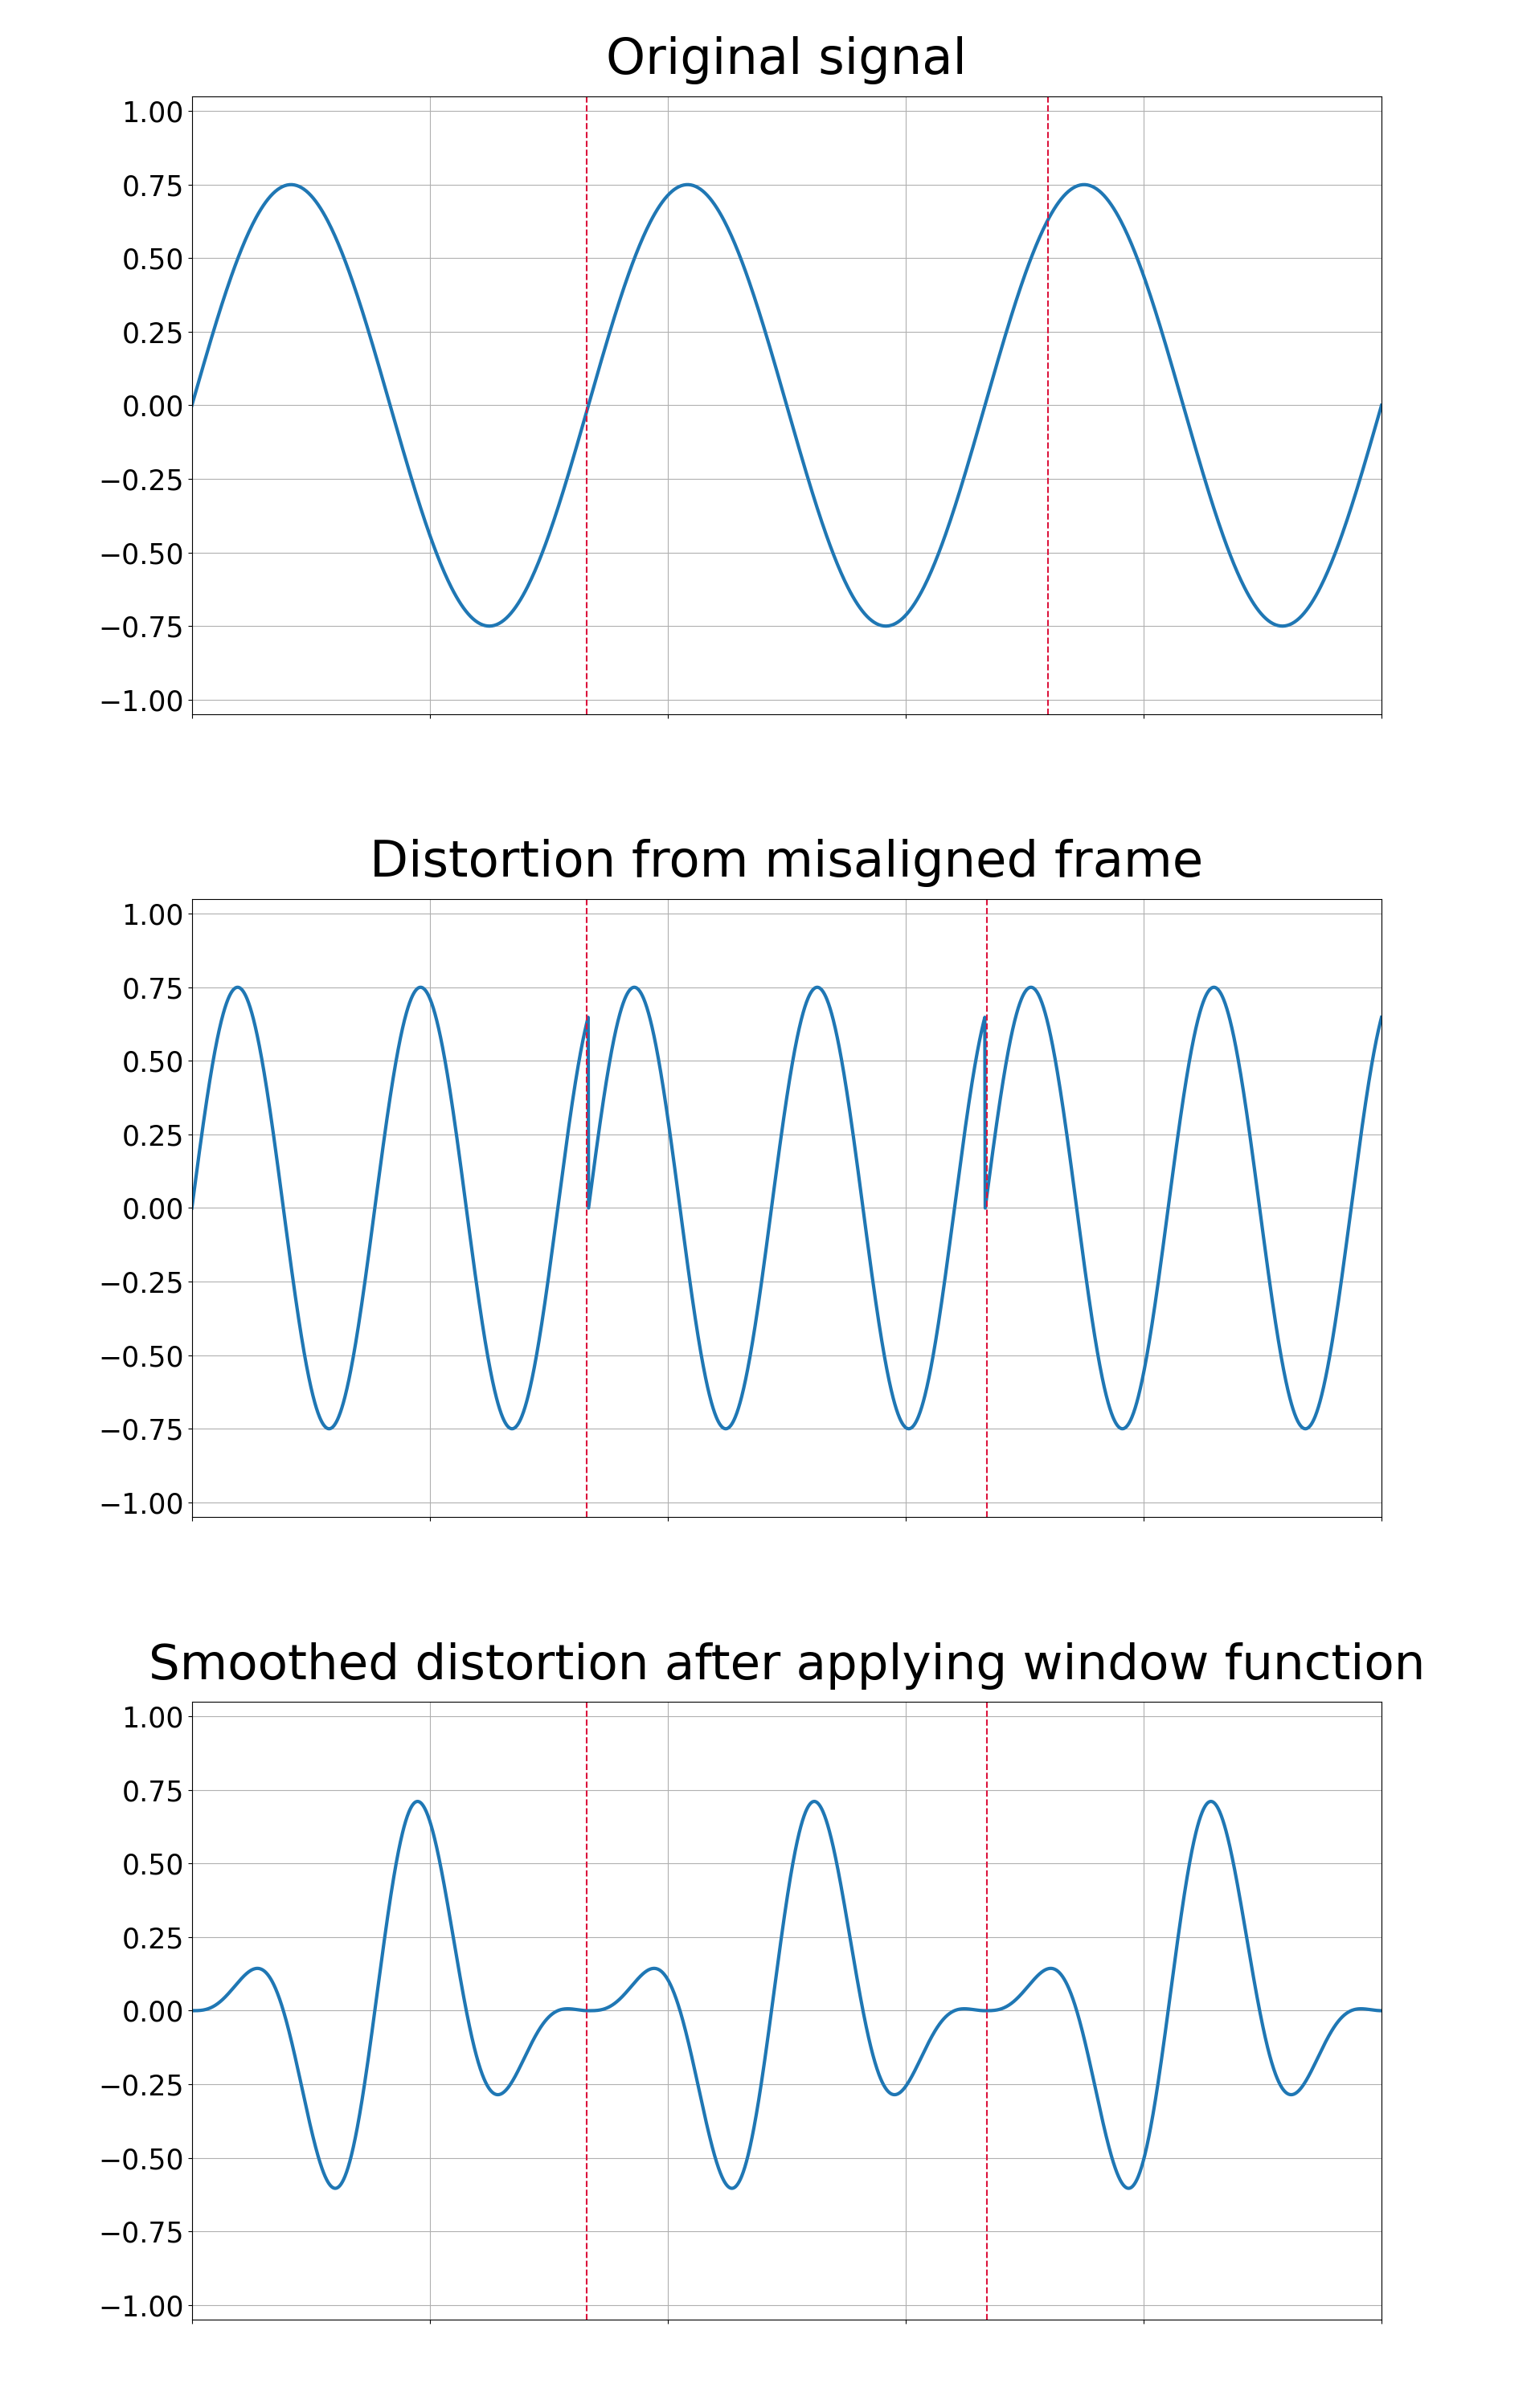
\includegraphics[width=\linewidth]{fig/framedistortion.png}
    \caption{Distortion caused by misaligned framing.}
    \label{fig:framedistortion}
\end{figure}
In our example, the distortion introduces high frequencies components from suddenly going up and down around the frame border. It also introduces low frequencies components, as the distance between two peaks within a frame is shorter than the distance between two peaks between frames. The introduction of these new frequencies is a form of spectral leakage, as the peak in the continuous spectrum corresponding to a frequency component leaks into multiple bins. We can smooth the distortion around frame borders by forcing the beginning and end of a frame to align. This is commonly done by applying a window function to the frame, which forces both ends of the frame to zero.

Given signal $s(n)$ and window function $w(n)$, we get the resulting windowed signal $\text{res}(n)$ using:
\[ \text{res}(n) = s(n) * w(n) \]
Figure~\ref{fig:windowfunc} shows the working of a window function on a frame graphically.
\begin{figure}[b!]
    \centering
    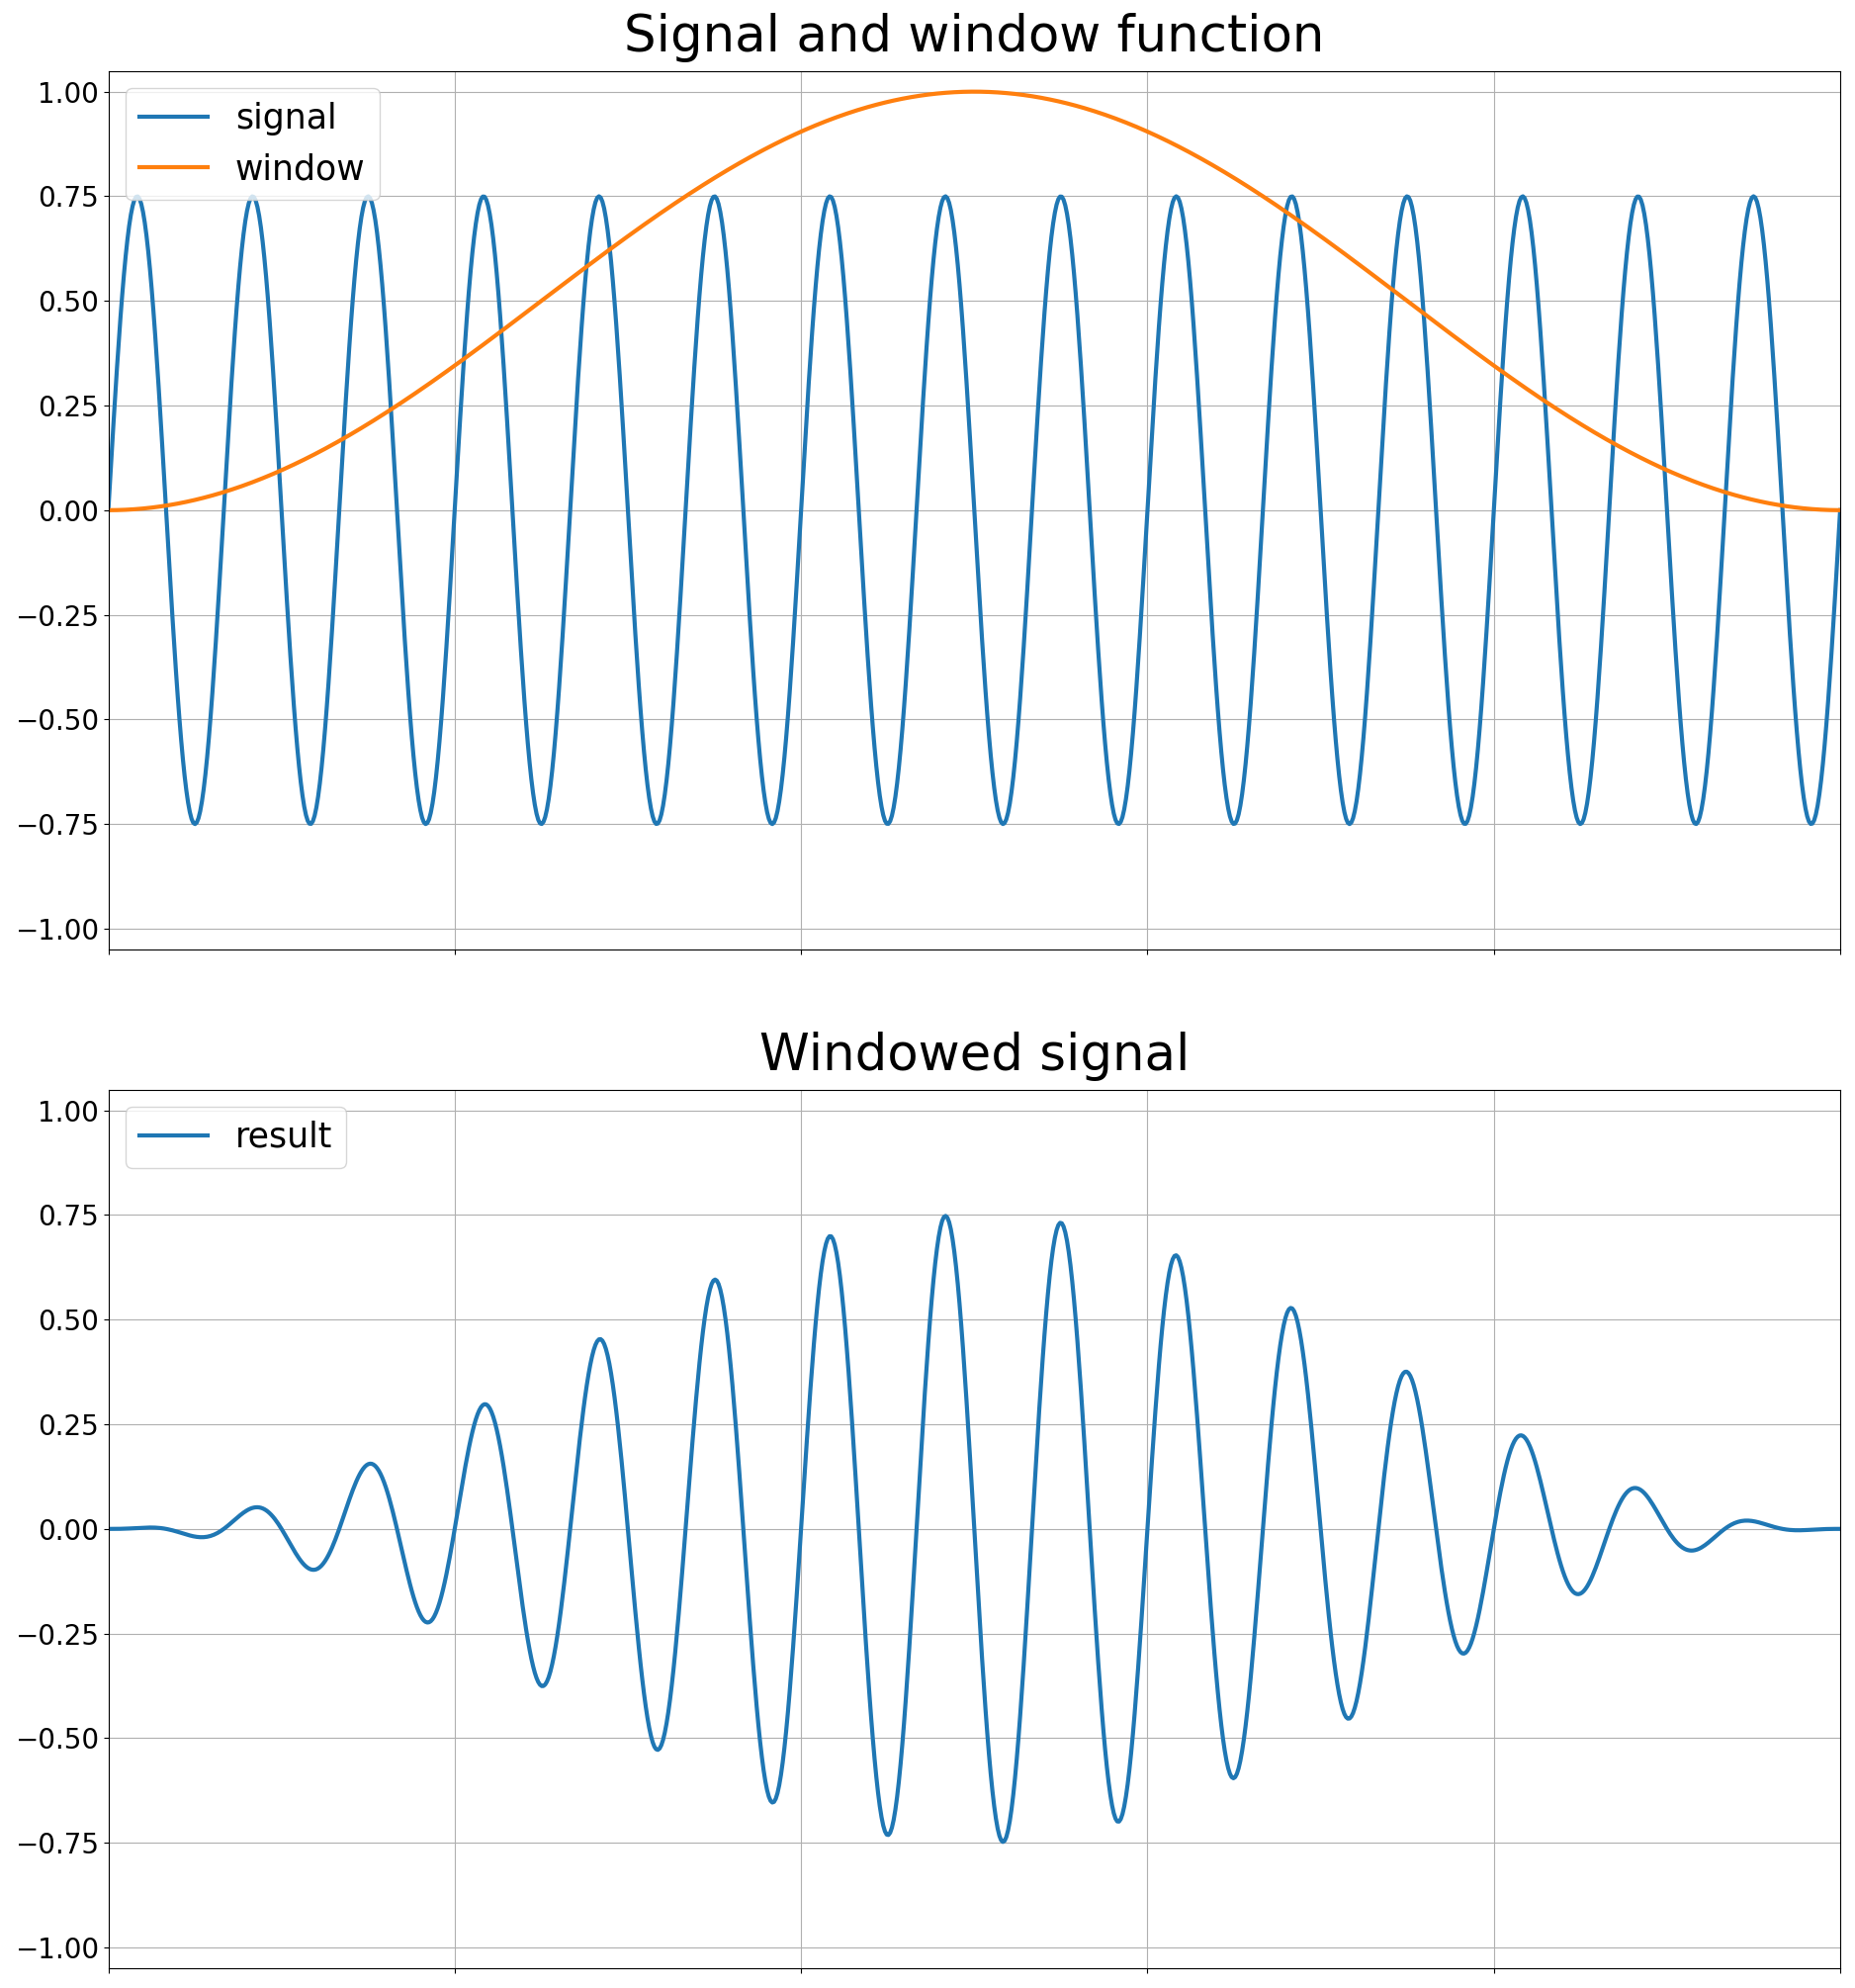
\includegraphics[width=\linewidth]{fig/window.png}
    \caption{An example of applying a window function to a signal.}
    \label{fig:windowfunc}
\end{figure}

The characteristics of spectral leakage from framing can be controlled using different window functions, see Figure~\ref{fig:windowfunceffect} for some examples. Applying no window function is referred to as using a rectangular window, as all the "wanted" samples from the signal are multiplied by 1 and all other samples by 0, effectively framing the signal.
%. We won't discuss individual window function in this section; see Appendix~\ref{sec:windows} for an in depth discussion on the different window functions.
\begin{figure}[b!]
    \centering
    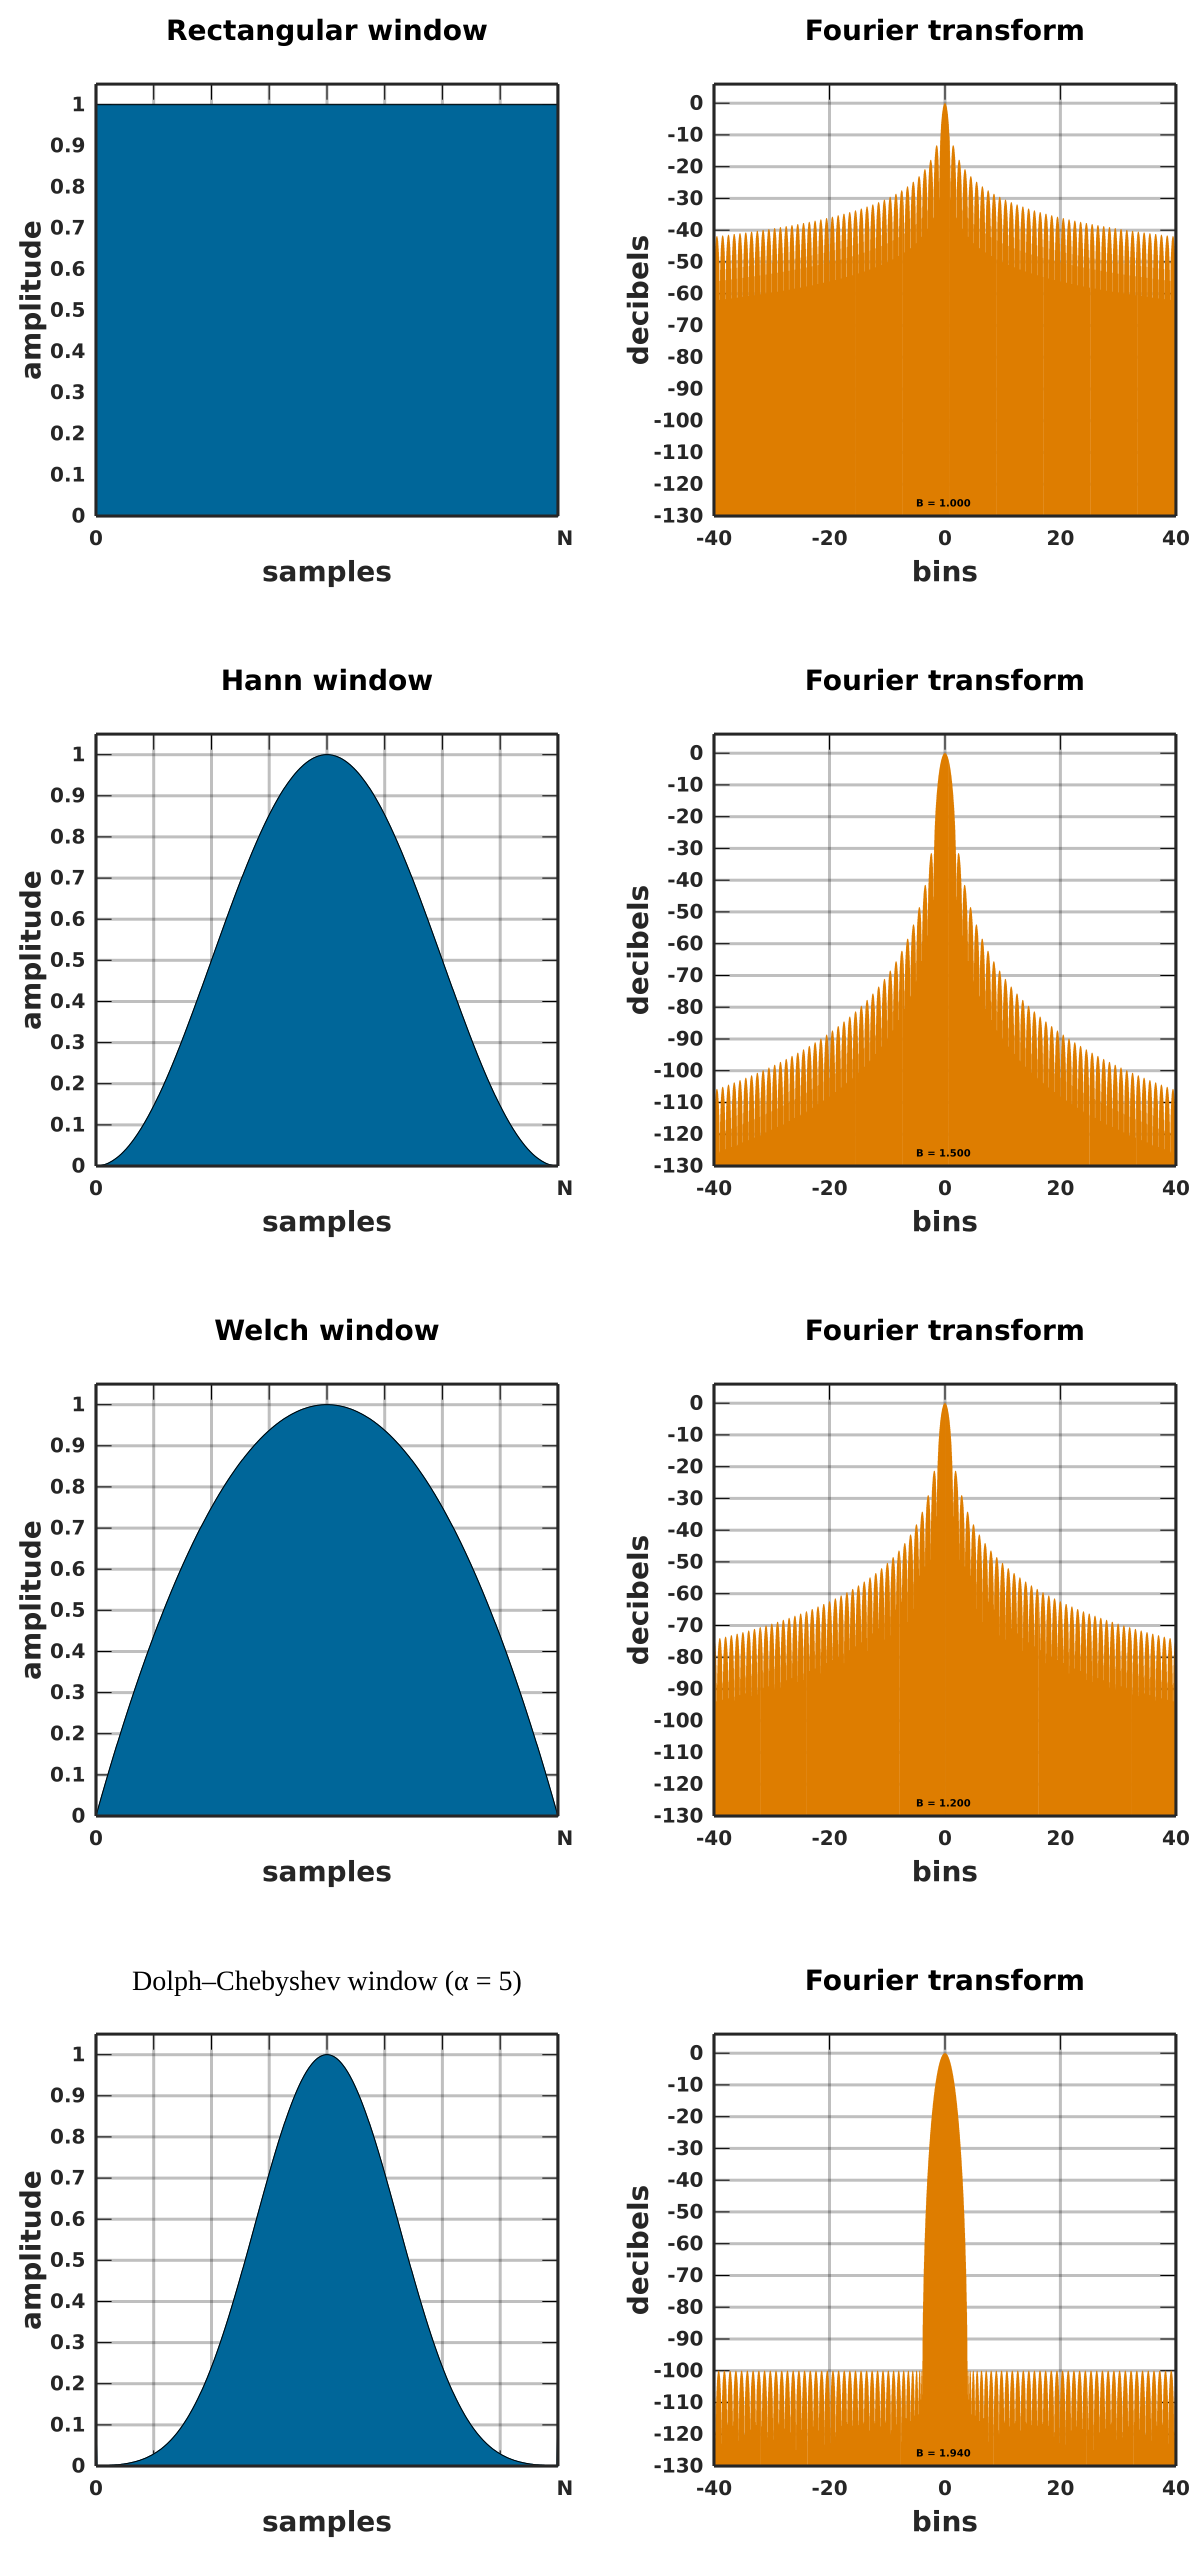
\includegraphics[width=0.92\linewidth]{fig/windows.png}
    % 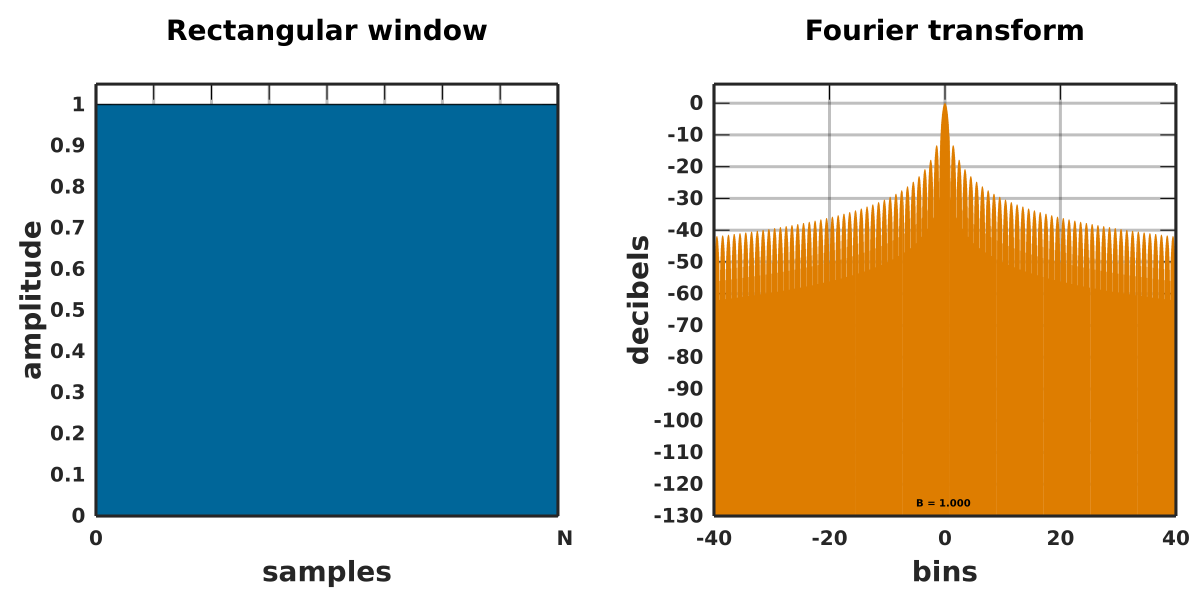
\includegraphics[width=\linewidth]{fig/window_rect.png}
    % 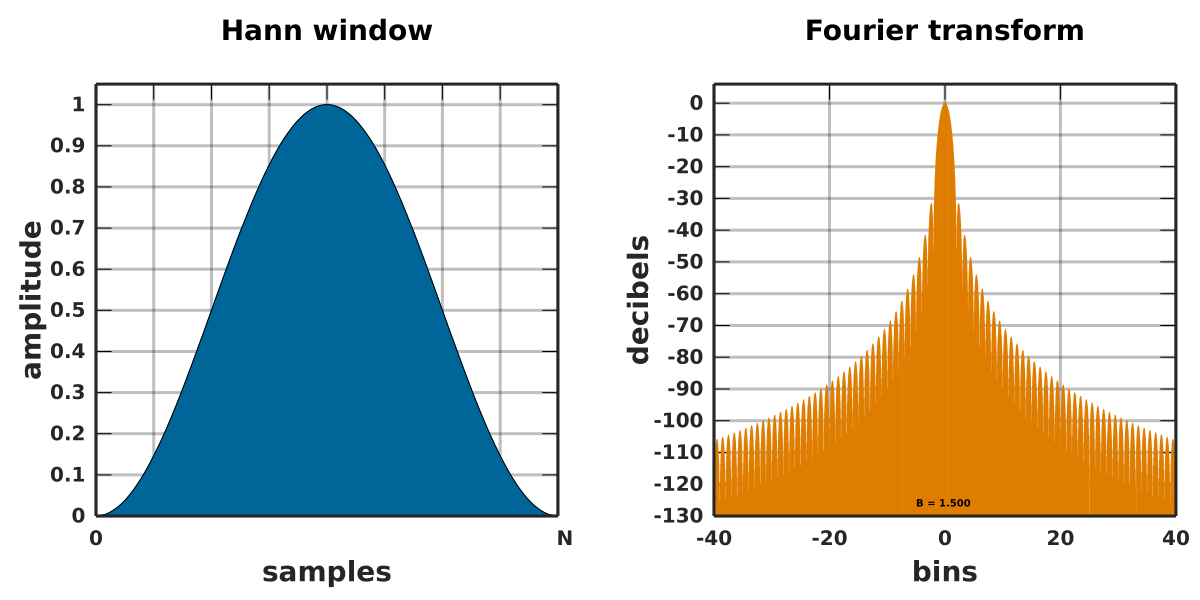
\includegraphics[width=\linewidth]{fig/window_hann.png}
    % 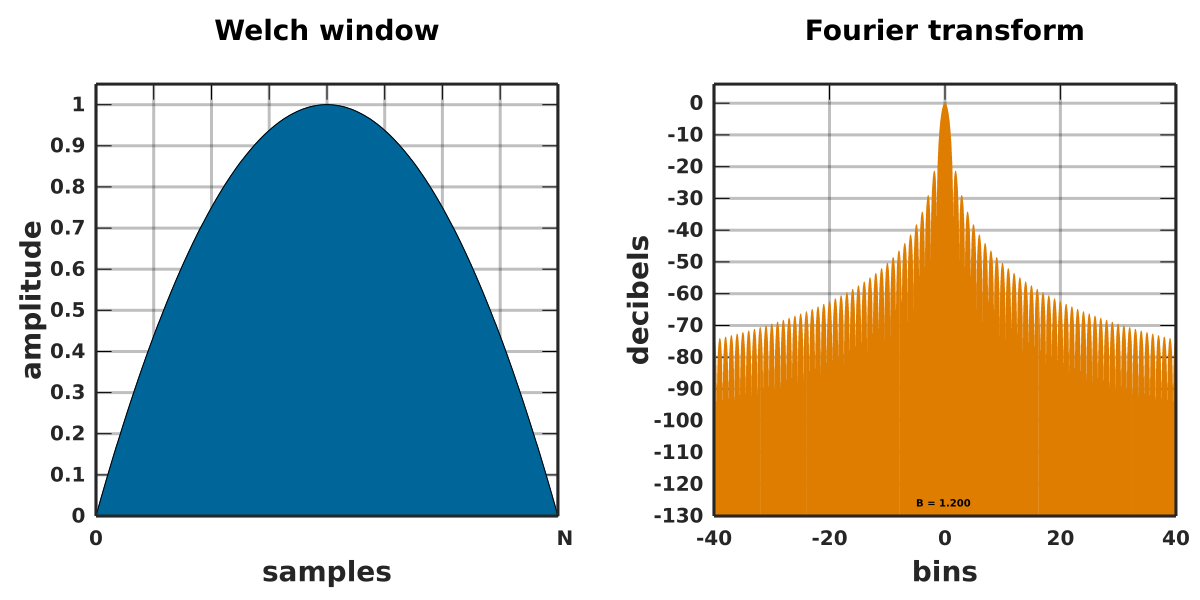
\includegraphics[width=\linewidth]{fig/window_welch.png}
    % 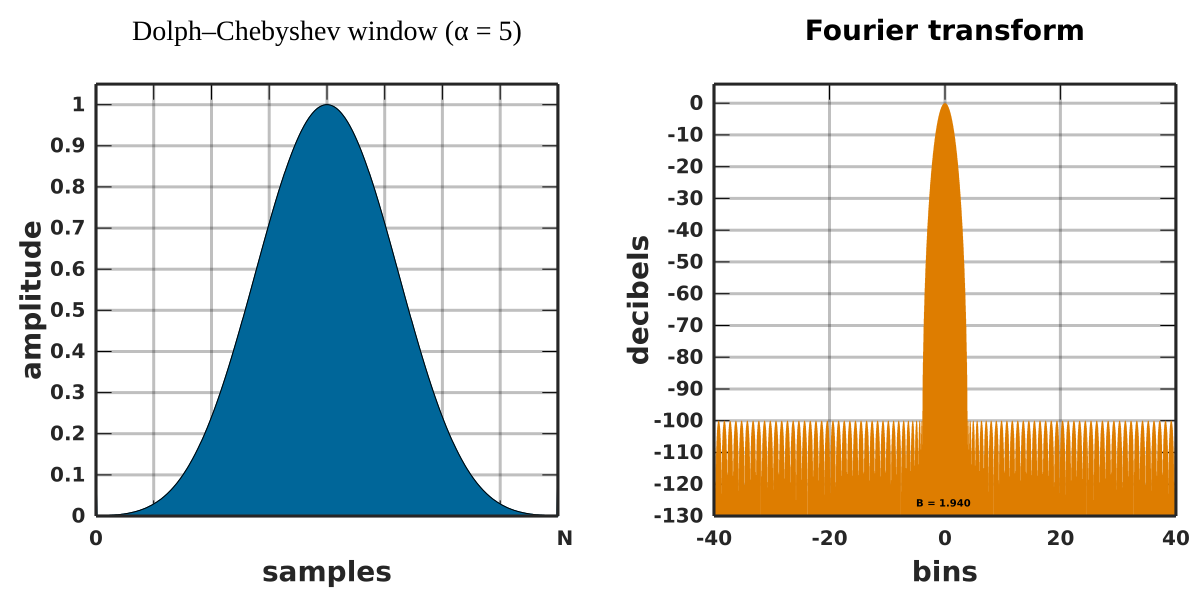
\includegraphics[width=\linewidth]{fig/window_dolph.png}
    \caption{Examples of the spectral leakage patterns of some window functions. On the left are the graphs of the different window functions and on the right the frequency response of the window function.}
    \label{fig:windowfunceffect}
\end{figure}

The leakage behavior of a window function can be quantified by performing a Fourier transform on the window function. The resulting frequency domain shows the amount of leakage in neighboring bins compared to the power of the center bin. To show the leakage behavior of frequencies which do not align with a bin, we can zero-pad the window function, which causes over-sampling in the frequency domain. Zero-padding is further discussed in Section~\ref{sec:zeropadding}. Figure~\ref{fig:winleak} shows the leakage of a rectangular window when a frequency exactly matches the center frequency of a bin and the leakage when a frequency is exactly between bins. Here we can see the leakage spectrum has lobes of leakage. The lobe containing the center bin is called the main lobe and the other lobes are called side lobes. The different window functions trade-off between having a narrow main lobe width and low side lobe levels~\cite{windowfunc}.
\begin{figure*}[b]
    \centering
    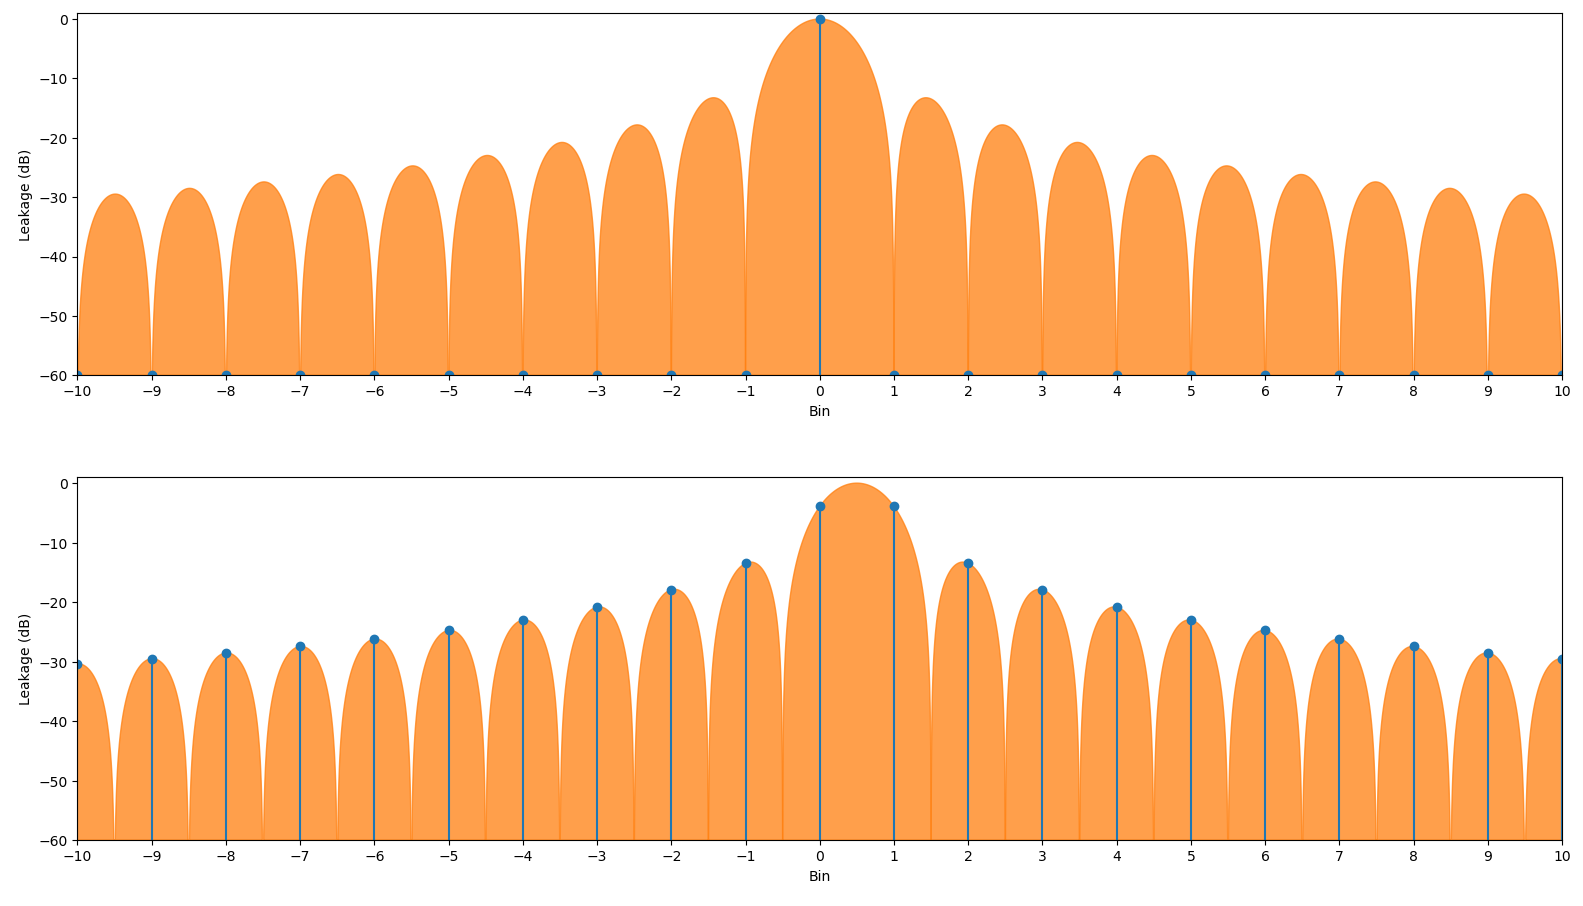
\includegraphics[width=\linewidth]{fig/winleak.png}
    \caption{Leakage behavior of the rectangular window. The orange lobes represent the frequency response of the rectangular window function; the blue lines represent the signal power measured in each bin. In the top plot, the frequency of the signal exactly matches the center frequency of a bin. Consequently, all signal power goes into the center bin and nothing into any other bin. In the bottom plot, we shifted the frequency response half a bin up to simulate a signal with a frequency exactly between bins. This causes signal power to diminishingly leak into all subsequent bins.}
    \label{fig:winleak}
\end{figure*}

% Window functions alter the amplitude of the original signal. This causes...
The performance of window functions is often described using equivalent noise bandwidth, coherent power gain and scalloping loss~\cite{windowperf3, windowperf2}. Equivalent noise bandwidth signifies the variation in noise floor compared to using a rectangular window. In other words, when transforming a signal, all the noise in the signal will result in some power in every bin, creating a floor in the spectrum. Window functions raise this noise floor by a consistent amount, which is quantified using equivalent noise bandwidth.
%
Applying a window function causes the overall amplitude of a frame to decrease, which in turn decreases the power of bins. This reduction is called the coherent power gain and signifies the loss of power in the spectrum.
%
As mentioned earlier, when a signal does not fit a frame, it leaks into other bins. Scalloping loss is the amount of decibel lost in the bin containing the main lobe when transforming a frame containing a signal halfway between bins compared to a signal containing the center frequency of a bin.

In order to accurately describe the signal power, we would need to correct for these effects. Equivalent noise bandwidth and coherent power gain can be described by a fixed value for each window function, but scalloping loss depends, along with the sample rate and frame size, on the spectral content of the signal, which we have no control over. Since absolute signal power estimations are not required for the content of this thesis, we will rely on relative power estimations instead.


\vspace{+4mm}
\subsection{Music theory and notation}
Modern western music uses the twelve-tone equal temperament (12-TET) music system. This system divides an octave, which is the interval between a pitch and another pitch with double the frequency, into twelve equally spaced semitones on the logarithmic scale. The logarithmic scale is used such that the perceived interval between two adjacent notes is constant~\cite{perception}. As a result, the ratio between two frequencies in an $n$-semitone interval is $\sqrt[12]{2}^n$ or $2^{\frac{n}{12}}$, invariant to pitch. A semitone can be further divided into 100 logarithmically scaled cents. %Cents are often used to measure the amount of dissonance.

Using scientific pitch notation, every note can be uniquely identified by combining the traditional note names \note{A}{} to \note{G}{} (optionally with accidentals such as $\sharp$ and $\flat$) with an octave number (e.g. \noteflat{E}{3}). An octave starts at \note{C}{}, which means the octave number increases between \note{B}{} and \note{C}{}. This counter intuitively implies \note{A}{3} is higher than \note{C}{3}. Note that in 12-TET, \notesharp{C}{} and \noteflat{D}{} are enharmonically equivalent. In this thesis, we will always refer to the sharp ($\sharp$) note instead of the enharmonically equivalent flat note ($\flat$). %Furthermore, even though technically \notesharp{B}{3} (which is equal to \note{C}{4}) is within the fourth octave, it is denoted to be in the third octave as accidentals do not change the octave number.
The range of a typical electric guitar in standard tuning is from \note{E}{2} up to \note{E}{6}.

The 12-TET music system only describes the relation between two notes in an interval. In order to play with other musicians in harmony, an arbitrary note has to be tuned to a specific frequency. Per ISO 16, the standard tuning frequency of the \note{A}{4} is 440 Hz within an accuracy of 0.5 Hz~\cite{isoa}. In this thesis, we will always assume a 12-TET music system with a 440 Hz tuning note.

Using the above information, we can translate frequencies into scientific note names and vice versa. In order to numerically work with note names, we assign a value to each note as shown in Table~\ref{tab:notenames}.
\begin{table}[h]
    \hfill
    \begin{center}
        \begin{tabular}
        {l|l}
            name & number \\
            \hline
            \note{C}{}      & 0 \\
            \notesharp{C}{} & 1 \\
            \note{D}{}      & 2 \\
            \notesharp{D}{} & 3 \\
            \note{E}{}      & 4 \\
            \note{F}{}      & 5
        \end{tabular}
        \qquad
        \begin{tabular}{l|l}
            name & number \\
            \hline
            \notesharp{F}{} & 6 \\
            \note{G}{}      & 7 \\
            \notesharp{G}{} & 8 \\
            \note{A}{}      & 9 \\
            \notesharp{A}{} & 10 \\
            \note{B}{}      & 11
        \end{tabular}
    \end{center}
    \hfill
    \caption{The numeric values encoding each note name.}
    \label{tab:notenames}
\end{table}

To make calculations easier, we use \note{C}{0} as a tuning note instead of \note{A}{4}. We can calculate the frequency of \note{C}{0} using the fact that \note{C}{0} is 57 semitones lower than \note{A}{4}:
\begin{align*}
    f_{C_0} = f_{A_4} * 2^{\frac{-57}{12}} &= 440 * 2^{\frac{-57}{12}} \\
                                           &\approx 16.352 \text{ Hz}
\end{align*}
% \[ f_{C_0} = 440 * 2^{\frac{-57}{12}} = 16.352 \text{ Hz} \]
% \[ 440 * \sqrt[12]{2}^{-57} = 16.352 Hz \]

We can calculate the frequency $f_{N_O}$, where $N$ is the note name which is represented by a numerical value given by Table~\ref{tab:notenames} and $O$ is the octave number using:
\begin{align*}
    f_{N_O} &= f_{C_0} * 2^O * 2^{\frac{N}{12}} \\
            &= f_{C_0} * 2^{O + \frac{N}{12}}
\end{align*}
% \[ f_{N_O} = f_{C_0} * 2^O * 2^{\frac{N}{12}} \]

To calculate the closest note $N_O$ corresponding to a frequency $f$, we first calculate the number of semitones $n_s$ between the tuning note $f_{C_0}$ and $f$:
\begin{align*}
    n_s = \round{12 * {}^{2}\!\log{\frac{f}{f_{C_0}}}}
\end{align*}
% Or more generally given a tuning note $N_O$:
% \begin{align*}
%     n_s^{N_O}(f) = \round{12 * {}^{2}\!\log{\frac{f}{f_{N_O}}}}
% \end{align*}
Here, $\round{\ldots}$ denotes rounding to the nearest integer. By rounding, we calculate the semitone distance to the note closest to $f$. Using this, we can calculate $N$ and $O$ as follows:
\begin{align*}
    N &= n_s \bmod 12 \\
    O &= \floor{\frac{n_s}{12}}
    % O &= n_s / 12
\end{align*}
Note that we assume $a \bmod b$ always return a number $c$ for which $0 \leq c < b$. Some programming languages allow the modulo operator to return a value $c$ for which $-b < c < b$, resulting in $-13 \bmod 10 = -3$ instead of $-13 \bmod 10 = 7$. Furthermore, when using a conversion to an integer instead of a floor, the octave number is rounded up when the note distance is negative.

In order to calculate the error $e$ (in cents) between the given frequency and the closest tuned note, we first calculate the tuned frequency $f_t$ of the closest note:
\[ f_t = f_{C_0} * 2^{\frac{n_s}{12}} \]
Then the error $e$ can be calculated using:
\[ e = 1200 * {}^{2}\!\log{\frac{f}{f_t}} \]

In digital music processing, notes are often represented through MIDI note numbers, as it allows programmers to refer to notes using integer values. The MIDI standard defines MIDI note number 69 to be the standard tuning frequency \note{A}{4}. Every semitone up/down respectively increases/decreases the MIDI note number by 1. This makes our tuning note \note{C}{0} number 12. According to the MIDI specification note numbers can take a value from 0 to 127, however, this is only relevant when communicating with MIDI devices. The following equations are valid for any note/MIDI note number.

The MIDI note number $m$ corresponding to the note closest to frequency $f$ can be calculated using the semitone distance from a frequency with a known MIDI note number. Let $m(N_O)$ denote the MIDI note number of $N_O$:
\begin{align*}
    m &= \round{12 * {}^{2}\!\log{\frac{f}{f_{N_O}}}} + m(N_O)% \\
      % &\approx \round{12 * {}^{2}\!\log{\frac{f}{16.352}}} + 12 \\
      % &= \round{12 * {}^{2}\!\log{\frac{f}{f_{C_0}}}} + 12
\end{align*}
Conversely, the frequency $f$ of the note corresponding to MIDI number $m$ can be calculated as follows:
\begin{align*}
    f &= f_{N_O} * 2^{(m - m(N_O)) / 12}% \\
      % &\approx 16.352 * 2^{(m - 12) / 12} \\
      % &= f_{C_0} * 2^{(m - 12) / 12}
\end{align*}
\vfill\pagebreak


% \subsection{Science of sound}  \label{sec:physsound}
\subsection{Physical properties of sound}  \label{sec:physsound}
The perceived loudness of a note over time can be described using an Attack Decay Sustain Release (ADSR) envelope. The ADSR envelope of a played note is the convex hull of the waveform of the signal, see Figure~\ref{fig:adsr} for an example. This convex hull can be divided into four parts: Attack, Decay, Sustain and Release. When a note is strummed on the guitar, a percussive sound is generated which causes a loud and sharp attack along with the note. This percussive sound quickly decays and only the actually fretted note will sustain. Finally, when the note is released, it dies out quickly.

The percussive sound generated when strumming a note is called a transient. Transients contain a high degree of non-periodic components. Because of this, transients appear very chaotically in the frequency domain and are often considered noise. As a transient is of high amplitude, it overshadows the note which will eventually sustain. Consequently, we cannot use the samples from a transient for Fourier based pitch estimation. This in turn increases our minimum latency, as we have to wait for samples which do not contain the transient anymore.

When playing a note on an instrument, many sine waves are generated. The most notable frequency is called the fundamental frequency and determines what note is actually played. Integer multiples of the fundamental frequency can resonate and give rise to harmonic overtones~\cite{overtones}. In practice, these overtones are not exact integer multiples due to non-linear effects resulting from the specific characteristics of the instrument.

Many other frequencies are generated along with the fundamental and its overtones. The instrument specific pattern of these frequencies, along with the characteristics of the overtones, is called the timbre of the instrument~\cite{timbre}. The timbre is what differentiates the sound of the same note played on two different instruments~\cite{perception}. Generally, the amplitude of the timbre frequencies is low compared to the fundamental frequency and can be disregarded as noise in the frequency domain. Figure~\ref{fig:timbre} shows the effect of timbre on a waveform.

In Section~\ref{sec:related}, we mentioned overtones are dissonant with respect to notes in 12-TET. This is true for all overtones, except for octaves, which is every $n$-th overtone where $n$ is equal to $2^i - 1$ for any integer $i$. In Table~\ref{tab:overseries}, we show an example for the overtones of \note{C}{4}. Note that the series of errors is always the same, regardless of what the starting note is. 
\begin{figure}[h]
    \centering
    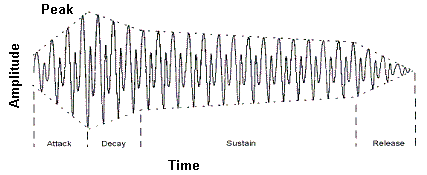
\includegraphics[width=\linewidth]{fig/envelope.png}
    \caption{Example of an ADSR envelope.}
    \label{fig:adsr}
\end{figure}
\begin{figure}[h]
    \centering
    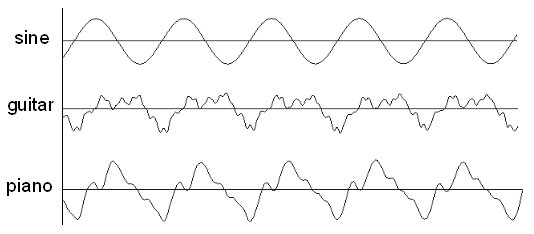
\includegraphics[width=0.95\linewidth]{fig/timbre.jpg}
    \caption{Example of difference in timbre between instruments compared to a sine wave.}
    \label{fig:timbre}
\end{figure}
\begin{table}[h!]
    \centering
    \begin{tabular}{rrcrr}
        $n$ & $f_{\text{overtone}}$ & closest note & $f_\text{note}$ & error \\
        \hline
        0 & 261.626  & $C_4$    & 261.626  &  - \\
        1 & 523.251  & $C_5$    & 523.251  &  0 \\
        2 & 784.877  & $G_5$    & 783.991  &  1.955 \\
        3 & 1046.502 & $C_6$    & 1046.502 &  0 \\
        4 & 1308.128 & $E_6$    & 1318.510 &  -13.686 \\
        5 & 1569.753 & $G_6$    & 1567.982 &  1.955 \\
        6 & 1831.379 & $A^\#_6$ & 1864.655 &  -31.174
    \end{tabular}
    \caption{Example of an overtone series from \note{C}{4} and the error of each overtone compared to its closest note.}
    \label{tab:overseries}
\end{table}

% We also mentioned in Section~\ref{sec:related} that, when using the CQT transform, none of the non-octave overtones coincides with a CQT bin as the CQT bins are exponentially spaced like the notes in a scale. This causes the frequencies of the overtones to spread out over bins, resulting in more noise in the frequency domain. Furthermore, overtones are important for discerning fundamentals from noise generated by transients. By using a Fourier transform tuned to a specific note, all its overtones are also coincide with Fourier bins. By performing a Fourier tuned to every note in the 12 tone scale, we can measure every note and its overtones.

% \textcolor{gray}{TODO: This thesis mainly focuses on monophonic pitch estimation, as it is much easier to perform. But we can still see how well our strategy works in the polyphonic case.
% TODO: A big problem in monophonic pitch estimation is the octave problem. Octaves are difficult to discern as the fundamental frequency and overtones of the higher note coincide with the overtones of the lower note. A similar problem arises
% TODO: The main problem in polyphonic pitch estimation comes from the occurrence of overtones. As mentioned before, notes in octave tend overshadow each other. Furthermore, as shown in Table~\ref{tab:overtones}, the overtones of a note can coincide with the...
% TODO: Overtone overlap and polyphonic difficulty.}
% \begin{table}[h]
%     \centering
%     \hfill
%     \begin{tabular}{r|l}
%         $n$ & $f^{C_3}_0*n$ \\
%         \hline
%         1 & 130.813 \\
%         2 & 261.626 \\
%         \textcolor{red}{3} & \textcolor{red}{392.438} \\
%         4 & 523.251 \\
%         \textcolor{blue}{5} & \textcolor{blue}{654.064}
%     \end{tabular}
%     \hfill
%     \begin{tabular}{r|l}
%         $n$ & $f^{E_3}_0*n$ \\
%         \hline
%         1 & 164.814 \\
%         2 & 329.628 \\
%         3 & 494.441 \\
%         \textcolor{blue}{4} & \textcolor{blue}{659.255} \\
%         5 & 824.069
%     \end{tabular}
%     \hfill
%     \begin{tabular}{r|l}
%         $n$ & $f^{G_3}_0*n$ \\
%         \hline
%         1 & 195.998 \\
%         \textcolor{red}{2} & \textcolor{red}{391.995} \\
%         3 & 587.993 \\
%         4 & 783.991 \\
%         5 & 979.989
%     \end{tabular}
%     \hfill
%     \caption{Overtones of C, E and G.}
%     \label{tab:overtones}
% \end{table}
% \begin{table}[h]
%     \centering
%     \begin{tabular}{c|c|c}
%         Note & $f$ & $\Delta f$ \\
%         \hline
%         $f^{C_3}_2$ & 392.438 & \multirow{2}{*}{0.443} \\
%         $f^{G_3}_1$ & 391.995 & \\
%         \hline
%         $f^{C_3}_4$ & 654.064 & \multirow{2}{*}{5.191} \\
%         $f^{E_3}_3$ & 659.255 &
%     \end{tabular}
%     \caption{Colliding overtones.}
%     \label{tab:diff}
% \end{table}


\subsection{Real-time}
Real-time is a difficult concept, as it has multiple definitions based on what field of research it is used in. As the formal definitions relate to very different concepts, it usually does not cause any problems. Problems arise when the term is informally used, as the vernacular definitions often miss an important aspect of the formal definitions of real-time, which causes statements made about systems which adhere to these vernacular definitions to be unreliable or useless. Here are a few examples of different definitions (vernacular definitions are marked bold red):
\begin{enumerate}
    \item Being synced with actual clock time (or wall time). This is for instance relevant when playing media such as audio and video. When such media is played at an incorrect speed, it could be considered distorted. The hardware which keeps track of the clock time is called a real-time clock.
    \item A system must response within a specified time constraint, which is called the real-time constraint or deadline. This constraint is usually a relatively short time. The definition originates from real-time computing and is relevant when making car airbags or airplane control systems. Failing to response within the real-time constraint leads to failures of the system. Real-time systems are often classified into hard, firm and soft real-time based on the impact of missing the deadline~\cite{realclass}.
    \bfseries\color{red}\item\color{black}\normalfont A system which can provide a result or feedback with no noticeable delay after receiving some input. Examples of such systems include graphical user interfaces or instant chatting/calling. There are no hard deadlines which the system has to respond within and the system does not fail if some delay does occur. Only user experience is slightly impacted. In the field of real-time computing, this is often referred to as near real-time.
    \bfseries\color{red}\item\color{black}\normalfont A system which can process data faster than it acquires data. This is technically not real-time, however, it is often used as such in academic literature. It is important for real-time systems to process data faster than it acquires data so it does not lag behind after some time, however, this is an implicit deadline. Not having this deadline explicit may lead to non-sensible expectations of the system.
\end{enumerate}
Even though the first definition is very relevant when working with audio, it is not relevant for us. The audio drivers of operating systems handle all timing for us. We simply have to wait for samples to be recorded and made available to our program. We only have to keep the sampling rate in mind when working with the samples as shown in Section~\ref{sec:fourier}.

% TODO: Maybe it's a firm real-time system. And usefulness degrades more if latency was higher.
In order to allow guitarists to use their guitar as a MIDI instrument, our system has to respond within a small time frame. On top of that, if the system fails to respond quickly enough, the usefulness of the result degrades, as timing is very important when playing an instrument. These restrictions would classify our system as a soft real-time system per definition 2. We choose a real-time of constraint of 20 milliseconds. We elaborate on this choice in Section~\ref{sec:constraint}.

Other work in real-time pitch estimation often uses the fourth definition of real-time. This is problematic when using Fourier transform based methods, as many papers choose large frame sizes to get a high resolution in the frequency domain. For instance, in order to discern the two lowest notes on a guitar which are 4.9 Hz apart, we would need a frame length of 204 milliseconds. This implicit deadline is well over our real-time constraint and would be unplayable for any musician. Other papers we found which do explicitly set a real-time constraint, choose very high constraints from 140 ms~\cite{sloomboi} up to 360 ms~\cite{sloomboi2}. These constraints were likely chosen with the inherent limits of their solutions in mind. It is very important to set a real-time constraint solely based on the expectation of the systems from an outside perspective. Real-time constraints chosen with the inner working of the system in mind are merely a measure of performance that is hoped to be achieved and claiming a system is real-time based on such constrains is considered fraudulent. We have found no Fourier transform based pitch estimation papers which choose a real-time constraint close to the latency of commercial guitar synthesizer solutions, such as the Axon AX 100 described in Section~\ref{sec:ax100}.



\section{Real-time Fourier transform based monophonic pitch estimation}
At the heart of our research lies a pitch estimation algorithm. The task of a pitch estimation algorithm is to convert a frame of samples to some representation of the notes contained in the frame. In this thesis, we will focus on spectral analysis methods of pitch estimation. Specifically, we focus on pitch estimation using the spectra obtained from frames using the Fourier transform.

% We will start with constructing a very basic pitch estimation algorithm. Then we will 

% \textcolor{gray}{When working in real-time, actions which are normally trivial have to be analyzed critically. For instance, sleep when retrieving samples from audio in, non-blocking overlap number of samples to carry over...}

% \textcolor{gray}{Actual research etc. Summary what was done in the research project which we build on. Notes on future work of research project.}

% \textcolor{gray}{As mentioned in Section~\ref{sec:related} and shown in our research project, the resolution in the frequency domain is not sufficient for spectral peak selecting methods. Given the info in preliminaries, we can tune Fouriers to specific frequencies.}


\subsection{Real-time constraint}  \label{sec:constraint}
Before we start constructing our pitch estimation system, let us first choose a real-time constraint. The goal of our pitch estimation system is creating a digital representation of the played notes so it can for example be used for software sound synthesis. Consequently, the real-time constraint should reflect the critical latency. This is the latency for which the delay between playing a note and receiving the feedback, such as hearing back the synthesized note, becomes problematic. The critical latency is highly subjective and may even differ between playing styles.
% Therefore, we will deduce a reasonable real-time constraint from multiple upper bounds stemming from different arguments.
% Therefore, we will deduce a reasonable real-time constraint from a few different arguments.
Note that our real-time constraint only considers pitch estimation latency. If we want to do anything with the pitch estimation results in real-time, such as synthesizing audio, additional latency will be introduced. For this reason, we should not put our real-time constraint right at the critical latency, but leave some headroom for the program using our estimated pitches.

Even though the critical latency is subjective, it is the factor determining if a real-time pitch estimation system is usable in a musical context. In order to determine the critical latency empirically, we created a tool called \textit{delayed playback}, which plays back recorded audio with an arbitrary latency. Using \textit{delayed playback}, we found a latency of 30 milliseconds is a reasonable latency at which we can still comfortably play many songs. \textit{Delayed playback} can also be used to verify if a real-time constraint chosen by someone else is reasonable by your own standards.% The tool is described in depth in Section~\ref{sub:playback_latency}.% Note that the reported latency from does not include the latencies introduced by the audio drivers and hardware discussed in Section~\ref{sub:computer_audio}.

% \textcolor{gray}{TODO: Rewrite paragraph, as playing faster is easier due to relying more on muscle memory instead of listening to yourself.}
% The critical latency depends, among other things, on the speed with which notes are played. For instance, let's assume a latency of 50 milliseconds. When playing a slow song consisting of quarter notes at 120 BPM, resulting in 2 notes per second, the latency is only a tenth of the note duration. However, when playing a fast solo consisting of sixteenth notes at 210 BPM, resulting in 12 notes per second, the latency is 70\% of the note duration. This means you hear more of the previous note than the current note for the duration with which the current note is played, which makes playing at fast speeds extra difficult. % This tricks the brain in such a way that it prevents you from staying on beat.

There is a limit on how fast we can estimate the pitch of a played note. For instance, when we consider transients noise, we have to wait for the transient to pass before we can gather samples containing the note. Then, we need enough samples such that the lowest bin of the DFT does not exceed the frequency of the lowest note. In the case of \note{E}{2}, which is 82.407 Hz, we would need a minimum frame length of $ \frac{1}{82.407} * 1000 = 12.135 $ milliseconds. Due to spectral leakage, using such small frame lengths is not feasible. %However, as outlined in Section~\ref{sub:waveform_packet}, we can translate this idea to the time domain. In practice, this would result in a minimum latency of 14 to 15 milliseconds.

In order to assess what we can reasonably expect from our system, we measured the latency of a commercial guitar synthesizer solution. This is described in depth in Appendix~\ref{sec:ax100}. Here, we found the Axon AX 100 MKII at best has a latency of 15 milliseconds when it is able to guess the note "the first try". Otherwise, the latency may reach up to 40 milliseconds.

% \textcolor{gray}{TODO: Note on unaccounted latencies (audio driver/hardware latencies).}
% A careful reader may have noticed we actually discussed two different latencies. We mostly reason about the latency of our pitch estimation system. However, when reasoning about the critical latency, latencies from the audio driver and hardware as discussed in Section~\ref{sub:computer_audio} do matter. \textcolor{gray}{TODO: Estimate on these latencies. Estimate of latency when running Digistring's algorithms on specialized hardware}.

% \textcolor{gray}{TODO: Our real-time constraint choice.}
Taking everything discussed in this section into account, we choose a real-time constraint of 20 milliseconds.

% \textcolor{gray}{Start with the factors coming into play when choosing the real-time constraint for our system (latency, played notes per second etc). Note on measured latency in Appendix~\ref{sec:ax100}. Empirically found bounds on latency using our latency program}


% \subsection{Software amplification}
% \textcolor{gray}{(Software representation of samples and FFT). The FFT works on floating point numbers but most audio interfaces give up to 24 bit integers...}
% \textcolor{gray}{We found empirically that when amplifying the input signal in software, peaks in the frequency domain are much easier to detect. However, it has to be done carefully to prevent distortion artifacts.}


\subsection{Basic algorithm for pitch estimation}  \label{sec:basic}
Let us start with constructing the most basic Fourier based monophonic pitch estimation algorithm. Given a frame of samples and the sample rate, the algorithm will return the MIDI number of the note closest to the most prominent frequency in the frame. First, we apply a window function to the frame and apply the Fourier transform. Then, we iterate over every output bin and check which bin has the highest magnitude. From the bin number, we can calculate the corresponding frequency and subsequently determine the note closest to this frequency. See Algorithm~\ref{alg:basic_pitch} for a pseudo-code implementation.
\input{pseudo_code/basic_pitch.pc}

To minimize our latency, we want to choose our frame size as small as possible while still being able to discern the two closest notes in frequency a typical guitar can produce. Due to the exponential nature of notes, the lowest two notes are always the closest two. For a typical guitar, these notes are \note{E}{2} and \note{F}{2}, which have a frequency of 82.407 Hz and 87.307 Hz respectively. This means we need a frequency resolution of at least $87.307 - 82.407 = 4.9$ Hz. This equates to a frame length of $4.9^{-1} = 0.204$ seconds, or 204 milliseconds. The bin centers do not have to exactly align with the notes to be able to discern them, so in practice we could get away with slightly shorter frames. Still, such large frame lengths are problematic for multiple reasons. A frame will contain multiple played notes when a guitarist plays at a moderate tempo (playing eighth notes in 150 BPM corresponds to 200 millisecond notes). Furthermore, if a frame contains the start of a note, the whole frame might be useless due to the transient. Lastly, since we have to wait until the audio driver has enough samples ready for us to fill a frame, the first samples from that frame will be 200 milliseconds old. The average latency of processing a sample is 100 milliseconds due to the frame length alone. This is well over our real-time constraint.

We implemented the basic Fourier pitch estimation algorithm in Digistring (\texttt{BasicFourier Estimator}). On average, the pitch estimation is performed in 0.13 milliseconds. This means our limiting factor is the long frame lengths, which implies we should look for methods which allow for accurate pitch estimation with lower frequency resolution. Furthermore, especially on low pitched notes, the basic estimator often picks the note one octave higher than the fundamental frequency. Apart from the octave errors, it does often produce correct results, however, it is completely infeasible for real-time usage due to the low frame rate. As we only produce one note estimate for every frame, we essentially quantize our estimator to eight notes on 150 BPM. Lastly, our basic estimator has no notion of silence. If no note is played in the frame, we essentially perform pitch estimation on white noise, giving us practically random note guesses.


\subsection{Overlapping frames}  \label{sec:overlapping}
As seen in the previous section, a low frame rate is problematic, as our note output rate is synced to the frame processing rate, essentially quantizing our note estimation to the frame processing rate. The straightforward solution would be to decrease the frame length, however, the frame length is limited by the minimum frequency resolution we need. Instead, we can increase the frame rate by partially overlapping subsequent frames.

Overlapping frames has several advantages. Apart from the increased frame rate, which in turn decreases quantization error, it may decrease the average latency of processing a sample. Furthermore, as transients are very short in the time domain, having more frames over a certain period of time decreases the relative number of frames containing the transient, which causes more frames to have a useful note estimate.%, see Figure~\ref{fig:overlap_transient} for a graphical explanation.
% \begin{figure}[h]
%     \centering
%     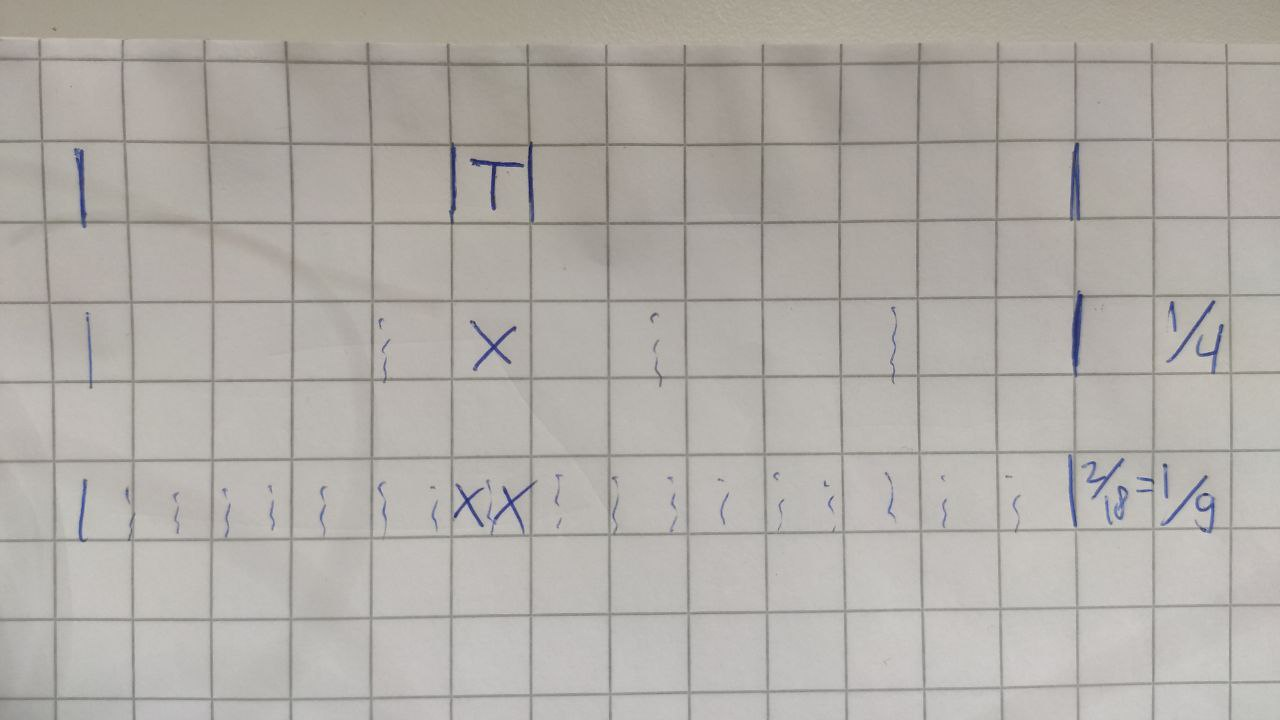
\includegraphics[width=\linewidth]{fig/overlap_transient.jpg}
%     \caption{\textcolor{red}{TODO: Correct image showing overlap instead of just shorter frames.} Given the signal given on top with a transient at T, relatively less frame estimations are ruined by the transient when using a higher frame rate.}
%     \label{fig:overlap_transient}
% \end{figure}

As two subsequent frames share information when overlapping, the estimation from subsequent frames is correlated. This limits the usefulness of overlapping beyond a certain overlap ratio~\cite{overlap}. However, as long as we do not overlap so much that samples are gathered faster than we can process them, overlapping does not incur an addition latency on the pitch estimation system.

When performing real-time estimation, instead of overlapping a constant ratio between frames, we can overlap based on the rate at which the audio driver acquires samples and our previous frame processing time. Time spend waiting for samples is effectively wasted time, as that time could have been spent on generating note estimations. Instead, we can always retrieve all currently available samples from the audio driver and fill the rest of the frame with samples from the previous frame. This ensures maximum possible overlap every frame.


\subsection{Zero padding}  \label{sec:zeropadding}
The number of output bins is determined by the number of samples that is transformed. We can artificially increase the number of samples in a transform by appending zeros to the frame. This technique is called zero padding. As only silence is added to the frame, it does not alter the spectrum.

As mentioned in Section~\ref{sec:fourier}, the frequency resolution of a DFT is $\Delta f_{bin} = \frac{f_{\text{SR}}}{n_F}$. Let $n_{F_P}$ be the zero padded frame size. Given that the sample rate is constant, our frequency resolution will increase by a factor of $\frac{n_{F_P}}{n_F}$. In other words, if we zero pad the frame such that it becomes $x$ times larger, our frequency resolution will increase by a factor $x$.

It is important to note that zero padding does not increase the resolution of the DFT, as no extra information about the original signal is added to the frame. It merely interpolates the coarse spectrum to become more smooth~\cite{zeropad1}. Two frequencies closer than $\Delta f_{bin}$ together form one big lobe in the smoothed spectrum. However, the interpolated peaks may have a higher amplitude than the original peaks, thus improving the results of our basic pitch estimation algorithm. See Figure~\ref{fig:visualpadding} for a graphical example of this.
\begin{figure}[b!]
    \centering
    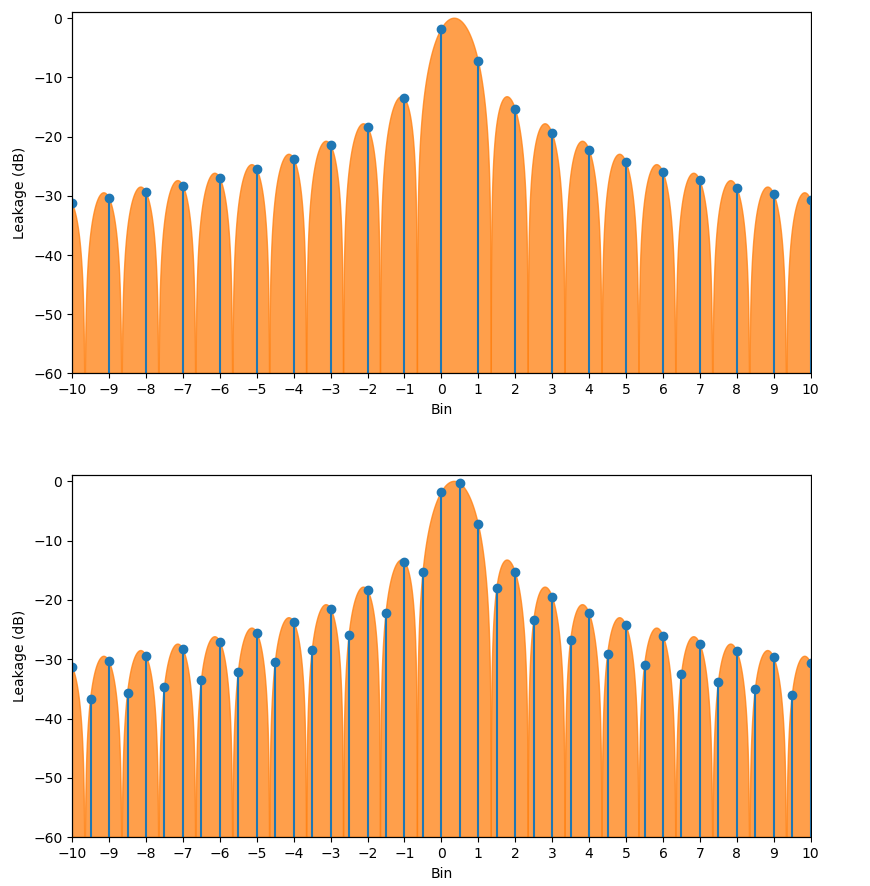
\includegraphics[width=\linewidth]{fig/zero_pad_interpolate3.png}
    \caption{The top and bottom figure show a DFT spectrum without and with zero padding respectively. Zeros are padded such that $n_{F_P} = 2 * n_F$ holds. The blue lines represent the bin magnitudes. The orange lobes represent the frequency content of the frame if infinite zero padding was applied.}
    \label{fig:visualpadding}
\end{figure}

Zero padding is relatively compute intensive form of interpolation~\cite{interpolnozero}. % The time complexity of the DFT is $O(N^2)$, where $N$ is the frame size. In the case of the FFT, the time complexity is reduced to $O(N \log N)$.
% \textcolor{red}{TODO: }\textcolor{gray}{For a length-N signal, the computational complexity of the Fast Fourier Transform (FFT) algorithm for calculating the DFT is O(N log N). So, zero padding a signal by a factor of D up to a length N D raises the cost by a factor D(logN D + 1). Zero padding by a factor D increases the cost of the algorithm by a factor that is greater than D—this is very expensive.}


\subsection{Quadratic interpolation}  \label{sub:qifft}
A less compute intensive method of interpolation is quadratic interpolation, also know as Quadratically Interpolated FFT (QIFFT)~\cite{interpolnozero}. Given a peak bin and its neighbors, QIFFT interpolates the actual peak location by fitting a parabola through these three points. The vertex of the fitted parabola is the interpolated peak location. See Figure~\ref{fig:qifft} for an example.

The accuracy of interpolation can be improved by performing the interpolation on a logarithmically weighted magnitude spectrum (LQIFFT). In other words, the error of interpolation is reduced if the logarithm of the bin power is used. Since a Gaussian curve is a parabola on a logarithmic scale, the interpolation is nearly perfect when using a Gaussian window function on a unweighted spectrum~\cite{interpolgaus}. It is not perfect, as a true Gaussian window would need infinite long tails~\cite{gauswin}.

Using an exponentially weighted magnitude spectrum (XQIFFT) may further reduce the interpolation error~\cite{interpolnozero}. However, this requires carefully choosing the exponent with which to weight the bins, as some choices may increase the error. As outlined in Section~\ref{sub:opt_xqfft}, we can iteratively approximate the optimal exponent. Note that the optimal value is specific to the exact pitch estimation strategy up to peak interpolation. For example, if the frame size, zero-padding factor or window function changes, the optimal exponent has to be approximated again. In Section~\ref{sub:exp:qifft}, we empirically derive the errors for the different interpolation methods. Note that the exponent factor cannot be zero.
\begin{figure}[b!]
    \centering
    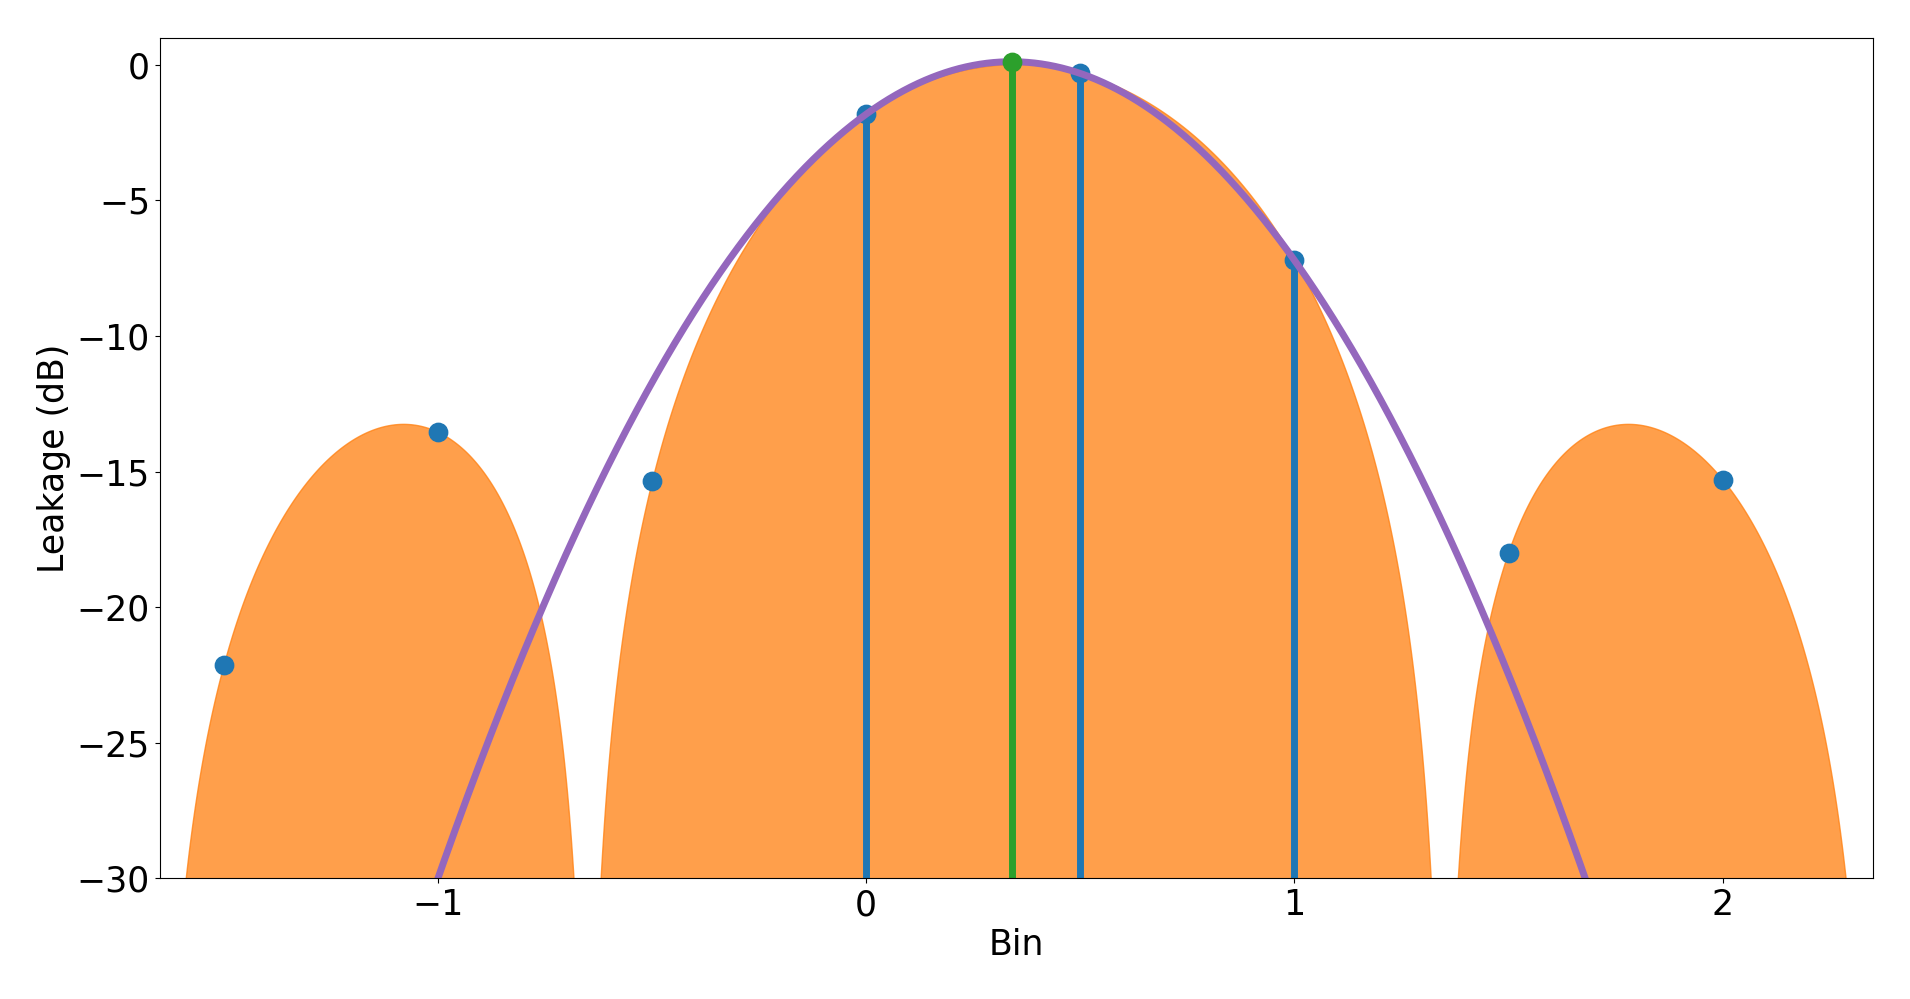
\includegraphics[width=\linewidth]{fig/qifft.png}
    \caption{Example of QIFFT. The three blue lines are the peak location and its neighbors, the purple line is the interpolation parabola and the green line represents the interpolated location. A zero-pad factor of 2 was used.}
    \label{fig:qifft}
\end{figure}

To perform quadratic interpolation, we calculate a value $p \in [-\frac{1}{2}, \frac{1}{2}]$, which is the offset in bins of the interpolated peak with respect to the peak bin $b_j$ at index $j$. Using the magnitude of the peak $|b_j|$ and the magnitude of the neighboring bins $|b_{j - 1}|$ and $|b_{j + 1}|$, we define:
\begin{align*}
    \alpha &= w(|b_{j - 1}|) \\
    \beta  &= w(|b_{j}|) \\
    \gamma &= w(|b_{j + 1}|)
\end{align*}
Here, $w(x)$ is an arbitrary weighting function. In the case of LQIFFT:
\[ w(x) = \ln{x} \]
Or in the case of XQIFFT with exponent $\epsilon$:
\[ w(x) = x^{\epsilon} \]
Then, we can calculate $p$ as follows:
\[ p = \frac{1}{2} \cdot \frac{\alpha - \gamma}{\alpha - 2\beta + \gamma} \]
The weighted amplitude $a_i^w$ corresponding to the interpolated peak is:
\[ a_i^w = \beta - \frac{(\alpha - \gamma) * p}{4} \]
The non-weighted interpolated amplitude is:
\[ a_i = w^{-1}(a_i^w) \]
Here, $w^{-1}(x)$ is the inverse of $w(x)$. In the case of LQIFFT:
\[ w^{-1}(x) = e^{x} \]
Or in the case of XQIFFT with exponent $\epsilon$:
\[ w^{-1}(x) = x^{\frac{1}{\epsilon}} \]
Given the bin number $j$ of the spectral peak location, the frequency $f_i$ corresponding to the interpolated peak is:
\[ f_i = \Delta f_{bin} * (j + p) \]
The Lagrange polynomial describing the interpolation parabola is defined as follows:
\begin{align*}
    % f(x) =\ & \sum_{n=-1}^{1} |b_{j + n}| \ \left(\prod_{j=-1, j \neq i}^{1} \frac{x - (j + m)}{(j + n) - (j + m)}\right) \\
    L(x) =\ & \sum_{n=-1}^{1} w(|b_{j + n}|) \ \left(\prod_{\substack{m=-1\\m \neq n}}^{1} \frac{x - (j + m)}{(j + n) - (j + m)}\right) \\
\\[-3mm]
         =\ & \alpha * \frac{x - j}      {(j - 1) - j}       * \frac{x - (j + 1)}{(j - 1) - (j + 1)} \\
         &+ \beta    * \frac{x - (j - 1)}{j - (j - 1)}       * \frac{x - (j + 1)}{j - (j + 1)} \\
         &+ \gamma   * \frac{x - (j - 1)}{(j + 1) - (j - 1)} * \frac{x - j}      {(j + 1) - j} \\
% \\[-2mm]
%          =\ & \alpha * \frac{x - j}       {-1} * \frac{x - (j + 1)} {-2} \\
%          &+ \beta    * \frac{x - (j - 1)} {1}  * \frac{x - (j + 1)} {-1} \\
%          &+ \gamma   * \frac{x - (j - 1)} {2}  * \frac{x - j}       {1} \\
% \\[-2mm]
%          =\ & \alpha * (j - x)              * \frac{x - j - 1} {-2} \\
%          &+ \beta    * (x - j + 1)          * (j + 1 - x) \\
%          &+ \gamma   * \frac{x - j + 1} {2} * (x - j) \\
% \\[-2mm]
%          =\ & \alpha * (j - x)                                     * (\frac{1}{2}j + \frac{1}{2} - \frac{1}{2}x) \\
%          &+ \beta    * (x - j + 1)                                 * (j + 1 - x) \\
%          &+ \gamma   * (\frac{1}{2}x - \frac{1}{2}j + \frac{1}{2}) * (x - j)\\
% \\[-2mm]
%          =\ & \alpha * (0.5x^2 - 0.5x - jx + 0.5j + 0.5j^2) \\
%          &+ \beta    * (-x^2 + 1 + 2jx - j^2) \\
%          &+ \gamma   * (0.5x^2 + 0.5x - jx - 0.5j + 0.5j^2) \\
\\[-2mm]
         =\ & \alpha * \frac{1}{2}(x^2 - x - 2jx + j + j^2) \\
         &+ \beta    * (-x^2 + 1 + 2jx - j^2) \\
         &+ \gamma   * \frac{1}{2}(x^2 + x - 2jx - j + j^2)
\end{align*}

One often overlooked detail is that the three interpolation points need to be in one spectral lobe as we approximate the shape of the lobe with a quadratic function. Most window functions have a wide enough main lobe, causing the three points to always be within the main lobe. In the case of the rectangular window, there are at most two bins within the main lobe. By zero padding, we can increase the number of bins in the spectrum and in turn get more than two bins in the main lobe, see Figure~\ref{fig:visualpadding}. In general, zero-padding decreases the error of quadratic interpolation~\cite{interpolnozero}.


\subsection{Peak picking}  \label{sub:pppeaakkk}
As explained in Section~\ref{sec:physsound}, overtones are generated along with the fundamental frequency when playing a note on an instrument. On the guitar, the first overtone is often measured as louder than the fundamental frequency, causing our basic pitch algorithm to report the first overtone instead of the fundamental frequency. This is referred to as the octave problem, as the first overtone is an octave from the fundamental frequency.

Instead of looking for the bin with the highest magnitude, we can try to identify all spectral peaks. Then, using these peaks, we can make a better estimate on what note is played in the frame.

Let us start with the most basic peak picker. Here, we return each bin which has two neighboring bins with a lower magnitude. This method does correctly identify all significant spectral peaks, but also finds many irrelevant peaks; especially in noisy areas of the spectrum, as there are many local maxima in random noise. For now, we can eliminate the peaks in noise by requiring a minimum peak power, but if the minimum value is not chosen carefully, the sustain of a note may be cut short. We need some method to select which peaks are significant.
% These noisy peaks could be filtered by requiring a minimal bin power before a peak is deemed significant, however, this doesn't work well in practice in a musical context. For instance, sustained notes will abruptly stop when the peak power goes below the threshold, which is detrimental for a cohesive musical experience. Furthermore, the optimal cut-off value for peak power is dependent on the used equipment and even the placement of the equipment. For example, an electric guitar receives much noise when in close proximity to wireless communication. For instance, having a phone in your pocket which is actively sending network packets or being close to a WiFi access point can result in loud, audible noise.

One way to determine if a peak is significant enough is Gaussian average envelope based peak picking~\cite{gausvelope}. Here, we first calculate a Gaussian weighted average envelope of the spectrum. Only peaks higher than the envelope are deemed significant. Figure~\ref{fig:gaus_env} shows the envelope filters insignificant peaks near large lobes caused by spectral leakage.

One envelope point is calculated for each bin in the spectrum. For each envelope point, we calculate the weighted average of all bins, where a bin's weight is determined by the number of bins between a bin and the bin corresponding to the envelope point. Given this distance $n$, the weight is calculated using a Gaussian function:
\[ w(n) = e^{-\pi (\frac{n}{\sigma})^2} \]
Here, the parameter $\sigma$ determines the relative weight of nearby bins compared to distant bins. Higher values for $\sigma$ causes nearby bins to have a higher weighting.
\begin{figure}[b!]
    \centering
    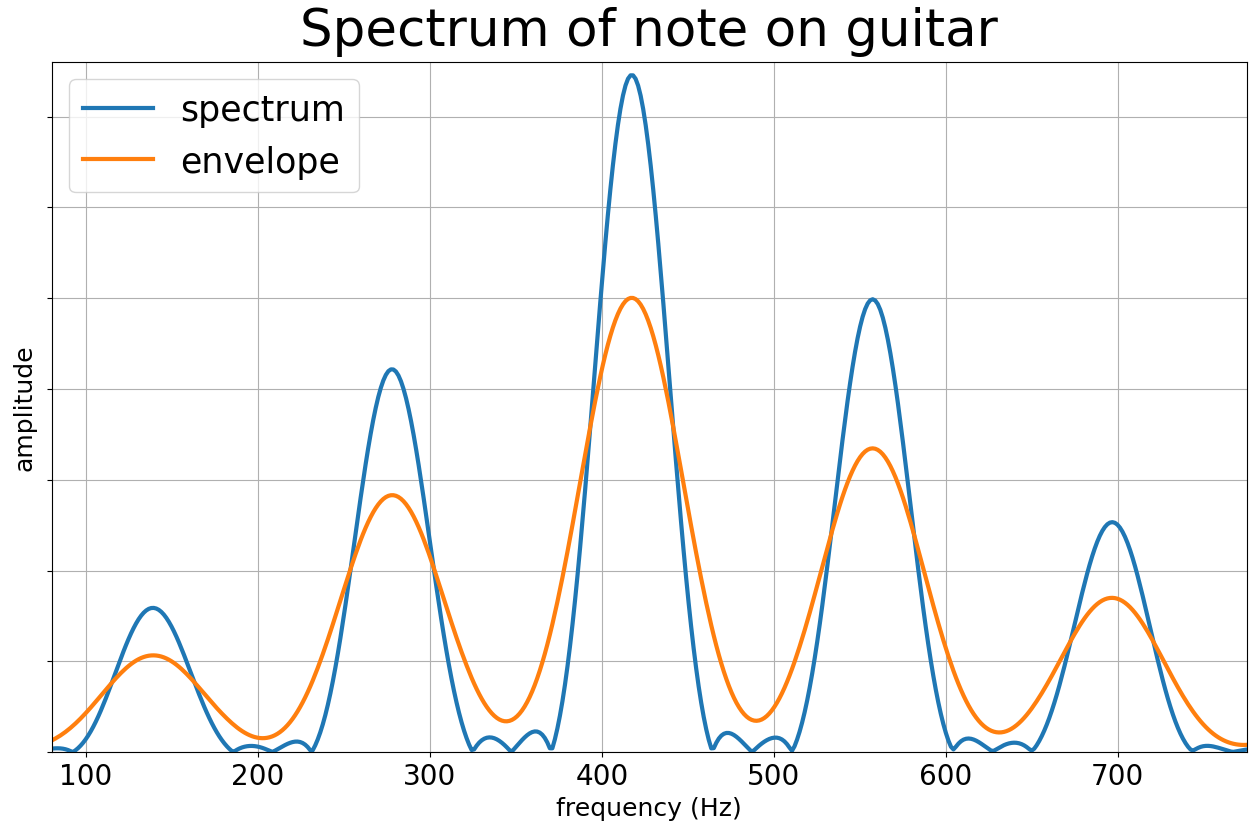
\includegraphics[width=\linewidth]{fig/gaus_spec.png}
    \caption{Example spectrum and its Gaussian envelope.}
    \label{fig:gaus_env}
\end{figure}

% As shown in Section~\ref{sub:expspeed}, Gaussian peak picking is an expensive process. As bin weights of far bins quickly become zero, we allow for a maximum kernel width to be set, which limits the number of bins to average. We set this number as a factor of the frame size and refer to it as the kernel width factor.
% As shown in Section~\ref{sub:expspeed}, Gaussian peak picking is an expensive process. As bin weights of far bins quickly become zero, we can omit these bins in our Gaussian average calculations. To control the number of bins used in calculating one envelope point, we allow for a maximum kernel width to be set. We set this number as a factor of the frame size and refer to it as the kernel width factor.
Calculating the Gaussian envelope is an computationally expensive process. As bin weights of far bins quickly become zero, we can omit these bins in our Gaussian average calculations, significantly decreasing the envelope computation time. To control the number of bins used in calculating one envelope point, we allow for a maximum kernel width to be set. We set this number as a factor of the frame size and refer to it as the kernel width factor. Furthermore, we can calculate envelope points in parallel for another significant speed-up.

% For an example of a Gaussian envelope, see Figure~\ref{fig:gaus_env}. Here, we can see the envelope filters the insignificant peaks near large lobes caused by spectral leakage.

% In large quiet parts of the spectrum, the envelope will also be close to the noise floor. To account for this, we allow for a minimum peak power threshold to be set, removing the peaks found in noise.


\subsection{Note selection from peaks}
Due to overtones and errors in peak picking, not every picked peak corresponds to a note in the signal. Therefor, we need an algorithm which can determine which note is likely being played given a set of significant peaks.

In our basic pitch estimation algorithm, we implicitly assume the loudest peak to be the fundamental frequency of the note contained in the frame. However, in practice, the first overtone may be louder than the fundamental frequency, causing octave errors. We could select the lowest peak as the fundamental frequency, however, this method is susceptible to low frequency noise.

Instead of selecting a single peak, we can look for a group of peaks which form a valid series of overtones, as played notes always come with overtones. As mentioned in Section~\ref{sec:physsound}, overtones are not exact integer multiples of the fundamental frequency, so we need to set a threshold on the maximum allowed difference. Because notes are separated exponentially in frequency, our threshold should scale accordingly. This is achieved by using cents as a measure of error. Then, we can either count the number of overtones for every peak and return the peak with the most overtones, or add the heights of the overtones up and return the peak with the highest overtone power. See Algorithm~\ref{alg:noteselect} for a pseudo-code implementation.

% We can make our note selection more resilient to noise by requiring a minimum number of overtones for a note to be selected. We removed this filter, as long sustained notes often have no more overtones, causing our note estimation to be cut short. However, if note tracking is implemented, one could only require the minimum number of overtones for new notes. As discussed in Section~\ref{sec:ax100}, the Axon also seems to perform this filtering.
We can make our note selection more resilient to noise by requiring a minimum number of overtones for a note to be selected. However, as a note sustains, overtones slowly fade out, which might cause the number of overtones to fall below the threshold, causing note estimation to be cut short. If note tracking is implemented, one could only require the minimum number of overtones for new notes. As we do not perform note tracking, we opted to disable this filter. As discussed in Section~\ref{sec:ax100}, the Axon also seems to perform this filtering.
%Furthermore, when playing two notes with no break in between, peaks from both notes are present in the spectrum due to overlapping. We can use this information to filter transients by requiring that the number
\input{pseudo_code/highres_overview.pc}
\input{pseudo_code/note_select.pc}


\subsection{Filtering}
As described in the previous sections, during most pitch estimation stages, we filter peaks/notes based on conditions such as minimal peak power or minimum number of overtones. Some filtering steps are however not necessarily tied to a specific estimation stage. For example, if we know a guitar only produces notes between \note{E}{2} and \note{E}{6} and the note selector selects a note outside if this range, the signal likely contains too much noise for an accurate estimation and we can discard the result. We refer to this filter as a range filter.

Similar to the minimum peak threshold during peak picking, we can also set a minimum signal power before we try to find notes in a frame. We refer to this threshold as the frame power threshold.

The biggest problem with threshold filters is that the threshold might not be a constant. For instance, if a guitarist switches from playing soft to loud, we need a higher threshold, as the noisy peaks will also increase in volume. As a consequence, we developed a signal-to-noise filter, which filters any peak with is softer than the loudest peak by some constant factor.

During transients, all note estimations are likely wrong. A straightforward method of detecting transients comes from the fact that transients occur at onsets, during which the signal power increases significantly. If the signal power in the current frame is some arbitrary threshold higher than in the previous frame, we assume the frame contains a transient. We could not report any note events in such frames, however, this increases the perceived estimation latency as the estimator will essentially wait until the transient has passed. Instead, we can have the estimator generate a special transient event, which synthesizers can use to generate a transient-like sound until a true note is estimated.
% Another important filter is a transient filter. During a transient, all estimations are likely wrong and it might be better to output nothing at all. An easy method of detecting transients comes from the fact that transients occur at onsets, during which the signal power increases significantly. If the signal power in the current frame is some arbitrary threshold higher than in the previous frame, we do not report any note events.


\subsection{High resolution estimator}  \label{sec:highrespitch}
We have put all of the above ideas together to create the HighRes estimator, see Algorithm~\ref{alg:highres_overview} for an overview. Its name stems from the general strategy it uses to perform pitch estimation, which is obtaining a high resolution frequency domain to approximate the continuous spectrum with.

Our estimator starts by applying a window function to the frame. We opted to use the Hann window function, as it strikes a good balance between a narrow center lobe and low leakage, however, changing the window function has little effect on the estimator's performance. Note that the frame is already zero-padded. This is done by creating a larger frame buffer than needed and zeroing the extra size once. As the zero-padded area should never be altered, it provides us with zero-padding for every frame. The window function only windows the non-padded part of the frame buffer. We then apply the Fourier transform on the frame buffer, giving us a frequency domain. This is converted to a spectrum by calculating the norm on every Fourier bin. From this spectrum, we create a list of peak locations using Gaussian peak picking. The peak locations are then refined using LQIFFT. From these interpolated peaks, we select the peak with the most overtones as our note estimation. %Lastly, we perform some filtering on the final result, such as range filtering.

Any of the functions in Algorithm~\ref{alg:highres_overview} can easily be replaced to create a different pitch estimation strategy, as long as the input and output is of the same kind. For instance, if we want to work on a logarithmically scaled spectrum, we can use a different \texttt{calc\_norms()} function which scales its output. Or we can change the peak-picking strategy to a non-Gaussian envelope based one by replacing \texttt{pick\_peaks()}.

Our HighRes estimator has many parameters which have to be tuned for a satisfactory result. The most important one is the \textit{frame size}. This determines the frequency resolution in our spectrum. The amount of zero-padding is determined by \textit{zero-pad factor}. The total frame size is determined by adding \textit{frame size} * \textit{zero-pad factor} to the frame size. In other words, \textit{zero-pad factor} determines the number of zeros to add to the frame size as a factor of the frame size. The amount of overlap is controlled using \textit{overlap factor}, which determines the number of overlapping samples by multiplying the frame size by this factor. To prevent peak picking on empty noise, we require a minimum signal power determined by \textit{power threshold}. Every peak also has a separate threshold \textit{peak threshold}. In the case of Gaussian peak picking, we use \textit{envelope threshold} instead. The envelope for Gaussian peak picking is controlled by \textit{sigma} and \textit{kernel width factor} as described in Section~\ref{sub:pppeaakkk}. Lastly, our signal to noise filter is controlled by \textit{signal to noise factor} and the range filter is controlled by \textit{lowest note} and \textit{highest note}.


% \subsection{Tuned Fourier transforms}
% \textcolor{gray}{12 Fouriers for each note and it's overtones.}



\section{Digistring}
% \textcolor{gray}{Details about the program I've written. Usage instructions, code choices, code structure, screenshots, expandability. TODO!!! Our framework provides scientist willing to research real-time pitch estimation an efficient implementation of many basic functions (e.g. efficient overlapping buffers, debug wave form generation, note synthesis based on estimation).}
%
Researching real-time pitch estimation is challenging. It is not necessarily difficult to implement some pitch estimation algorithm, however, such an implementation would essentially be a black box, as the resulting note estimation does not provide any information on how this estimate came to be. As outlined in Section~\ref{sec:highrespitch}, our pitch estimation algorithm has multiple stages all with multiple parameters which affect the performance of subsequent stages. Since we have extremely limited resolution in the frequency domain, it is very important all these parameters can be tuned carefully in order to minimize latency. This requires extensive feedback from the estimation process. Moreover, setting-up automated experiments is very time consuming, often causing research to only include some informal tests to verify the performance of their pitch estimation systems.
% Pitch estimation research has a high barrier of entry, especially the real-time case. It is not necessarily difficult to implement some pitch estimation algorithm, however, such an implementation would essentially be a black box, as the resulting note estimation does not provide any information on how this estimate came to be. As outlined in Section~\ref{sec:highrespitch}, our pitch estimation algorithm has multiple stages all with multiple parameters which affect the performance of subsequent stages. Since we have extremely limited resolution in the frequency domain in order to minimize latency, it is very important all these parameters can be tuned carefully. This requires extensive feedback from the estimation process. Moreover, setting-up automated experiments is very time consuming, often causing research to only includes some informal tests to verify the performance of their pitch estimation systems.

To combat these problems, we set out to create a pitch estimation framework called Digistring. This framework includes efficient implementations for all concepts described in this thesis, extensive graphical and auditory feedback of the estimation process, the ability to read samples from the audio driver or a file, tools for automated testing/performance measuring and an abstraction for pitch estimators such that all these features work with any arbitrary pitch estimation algorithm. Even though this thesis focuses on monophonic pitch estimation, Digistring supports both monophonic and polyphonic pitch estimation.

Digistring is implemented in \cpluspluslogo, as it is a high performance language suited for real-time systems. It uses FFTW3 for efficient Fourier transforms and SDL2 for graphics and audio. These libraries have been chosen, as they are both available on most Linux distributions. Digistring is available at \url{www.github.com/lucmans/digistring}.


\subsection{Digistring overview}
\begin{figure*}[t]
    \centering
    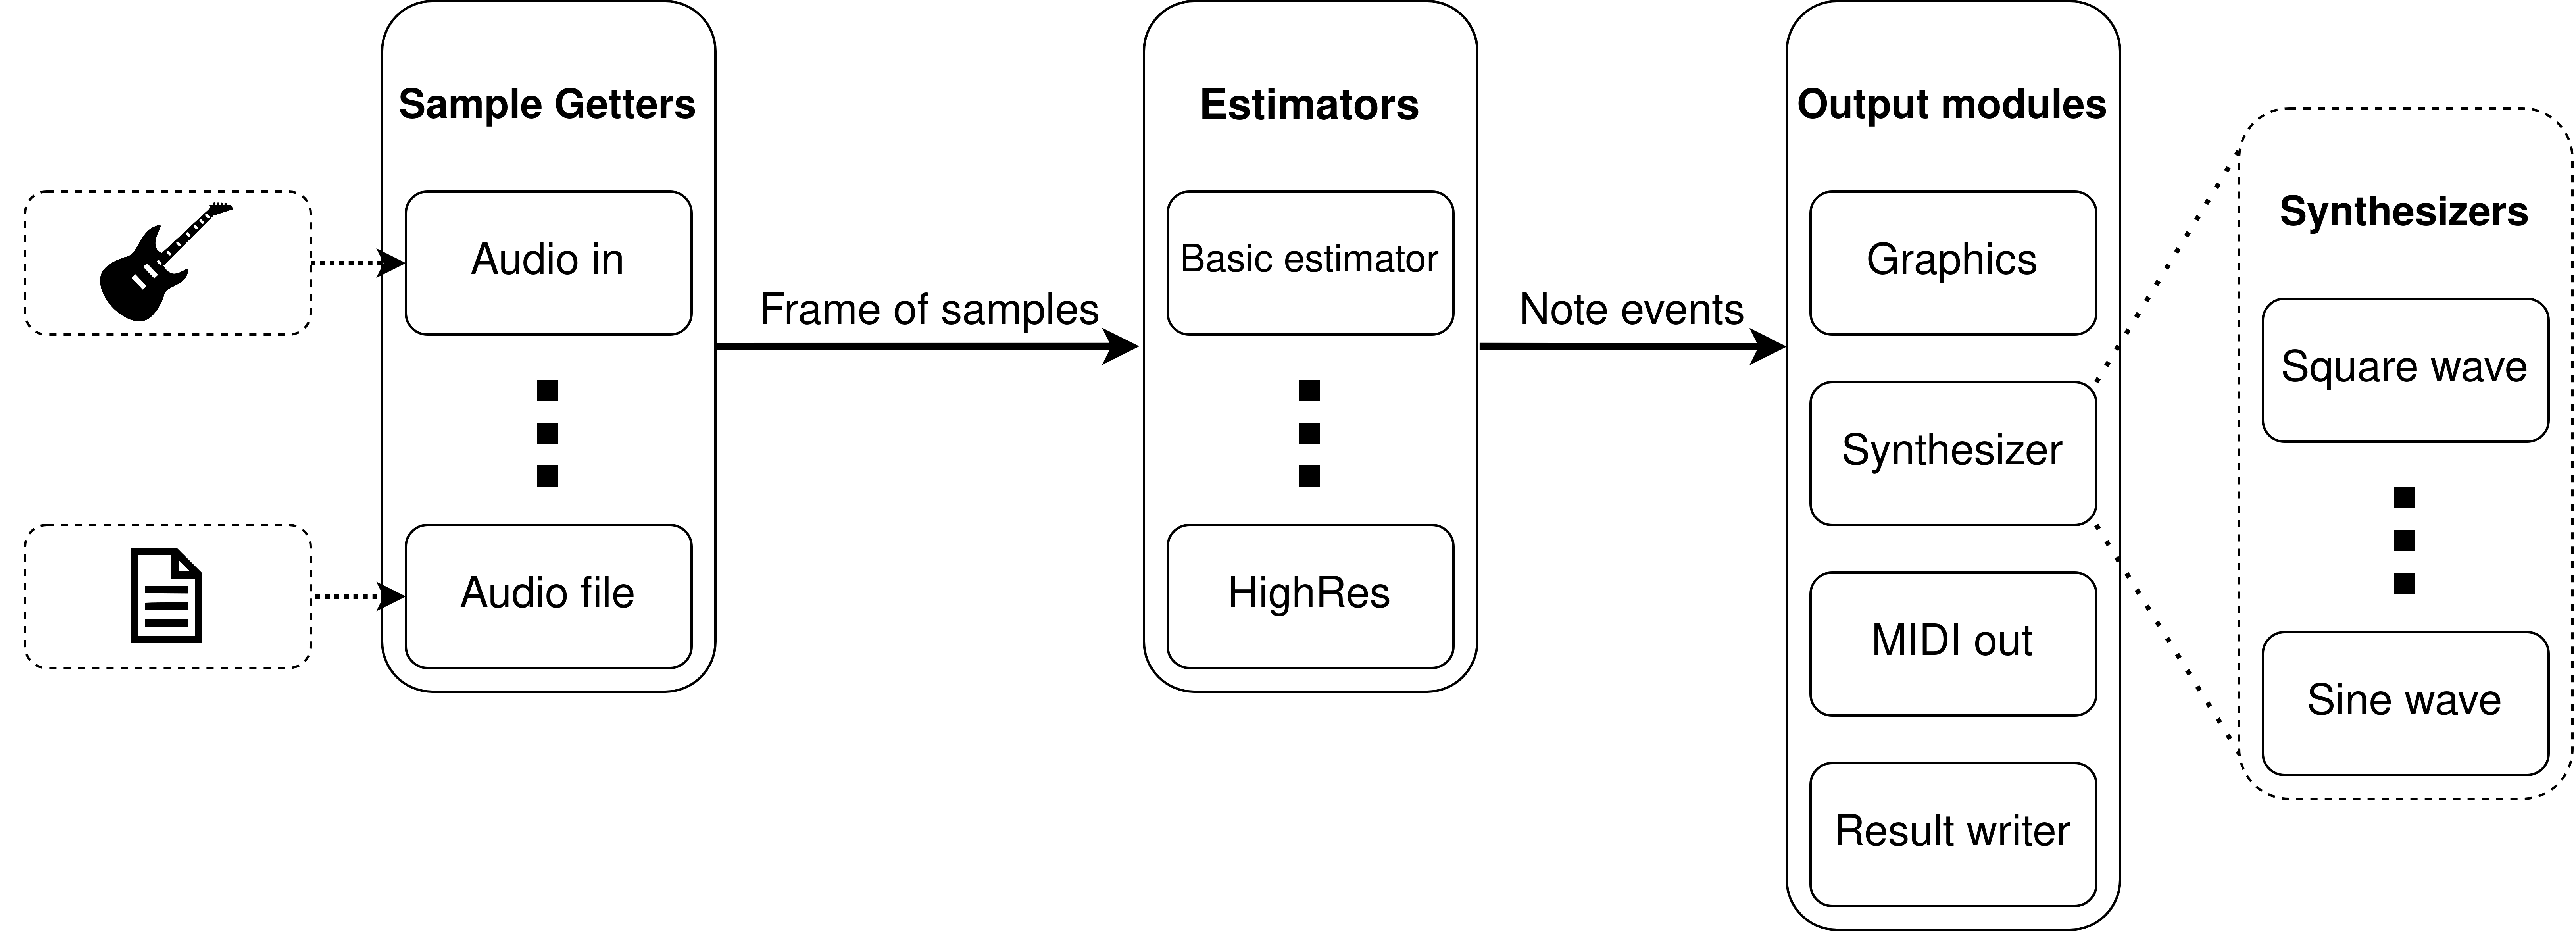
\includegraphics[width=0.85\linewidth]{fig/digistring_overview2.png}
    \caption{Overview of Digistring. The samples getters, estimators and synthesizers support being extended.}
    \label{fig:digistring_overview}
\end{figure*}
Digistring is divided into three main components, shown graphically in Figure~\ref{fig:digistring_overview}. The first is the sample getter, which as the name implies, retrieves samples from a sample source. The samples are then given to the pitch estimator, which transform the frame of samples to a note event list. A note events consists of a note and onset/offset information relative to the frame start. Lastly, the constructed note event list can be used by the different output modules. For instance, we can generate a JSON formatted file representing all the note events, which can in turn be used for automated testing. Digistring also features a synthesizer module, allowing us to verify if the results are, musically speaking, satisfactory. Certain small errors may completely negate the usefulness of any application of the pitch estimation algorithm. Furthermore, some technical errors may actually be of musical value. For instance, the random estimations during loud transients cause our synthesizer to produce a percussive sound effect, highlighting the loud transient.%, as was the case for guitar distortion, which is now one of the most widely used guitar effects.


\subsection{Estimator}
% \textcolor{gray}{Implementation details about estimator and estimator graphics. As an optimization, we share the input buffer of the estimator with the sample getter. This prevents a copy of the full frame every cycle.}
%
The main task of the estimator abstraction is separating pitch estimation from the rest of Digistring, such that the pitch estimation algorithm can easily be replaced. The goal of a pitch estimation algorithm is to convert a frame of sampled audio data to some representation of the notes contained in the frame. Consequently, the interface for an estimator should be a frame of samples as input and note events as output. A note event consists of a note along with onset/offset information expressed as number of samples relative to the start of the frame. Optionally, Estimators can set a confidence level for each estimated note events.

Estimators are split up in two phases: the initialization phase and estimation phase. The goal of the initialization phase is alleviating as much work as possible from the estimation phase, which minimizes latency. Examples of initialization phase tasks are precomputing the window and Gaussian function, setting up zero-padding buffers and letting FFTW3 optimize the used FFT algorithms.

When using zero-padding, the window function should be applied as if the input buffer was not zero-padded. In general, any modification to the input signal should never affect the zero-padding. Consequently, the padding only has to be zeroed in initialization phase, as it should never be overwritten.

As discussed in Section~\ref{sec:fourier}, we do not perform absolute signal power estimation. Instead, all note amplitudes reported by an estimator are on an arbitrary scale. As a consequence, output modules need to keep track of the maximum reported amplitude to which a specific note's amplitude can be compared to.

% The main estimator developed for this thesis is the high resolution estimator, which we refer to as the HighRes estimator. Its name stems from the general strategy it uses to perform pitch estimation, which is obtaining an as high resolution frequency domain as possible to approximate the continuous spectrum with.% \textcolor{red}{Implementation details.}


\subsection{Sample getter}  \label{sub:samplegetter}
As mentioned in Section~\ref{sub:computer_audio}, audio samples can be represented in different formats. Floating point samples have many advantages over integer or fixed point samples~\cite{dspfloat}. Most audio interfaces and audio file formats support 24 bit integer samples or 32 bit floating point samples as the best quality samples. Note that 24 bit integer samples can be converted lossless to 32 bit floating point samples. One could convert to 64 bit floating point samples, which slightly reduces the accumulated floating point rounding errors during digital signal processing. However, the accumulated error is negligible and it would require us to always convert any input samples. Using our tool \texttt{float\_vs\_double}, we found no difference in normal sample processing speed between 32 bit and 64 bit floating point numbers, but this may differ per CPU architecture. When using vector instruction sets such as AVX, the amount or parallelism is limited by the number of bits in the vector registers. As FFTW3 uses these vector instructions, 32 bit floating point number are faster. This can be verified using our \texttt{float\_vs\_double\_fftw3} tool. Given these arguments, we decided to use 32 bit floating point samples for all our samples processing in Digistring.

Frame overlapping, as discussed in Section~\ref{sec:overlapping}, is implemented in the sample getter. This way, the pitch estimator does not need to know about overlapping. Furthermore, by implementing overlapping in the base class, any newly added sample getter will automatically be able to overlap. There are two different overlapping strategies. The first overlaps two subsequent frames by a constant factor between 0 and 1. The number of samples to overlap is the frame size multiplied by this factor. We clamp the resulting number between 1 and frame size - 1 to assure we always overlap at least one sample or at least get one new sample. The second overlapping strategy is only applicable when reading samples from an audio device. Here, the number of overlapping samples is determined by subtracting the number of samples ready to be read from the audio driver from the frame size. The rest of the frame is filled with samples from the previous frame. To limit the amount of overlap, we allow for a minimum and maximum overlap factor to be set. In live usage, the minimum overlap factor should never be met, as it implies that the estimation system cannot keep up with the incoming samples from the audio driver. In Digistring, we refer to this second overlapping strategy as non-blocking overlap, as we try to overlap as much as possible without blocking on retrieving samples from the audio driver.%, as we try to overlap such that we won't block on retrieving samples from the audio driver.

A simple overlap implementation would save a copy of the entire input buffer, see Figure~\ref{fig:overlapgraph} for a graphical overview of the algorithm. As we know the amount of overlap, or at least an upper bound in the non-blocking case, we can only copy over what we might need next frame. This saved us both time and space, as less data has to be stored and less data has to be copied over. This does however force the sample getter to never request more samples in subsequent "get sample" calls, and in turn, it prevents using a variable overlap strategy. Using our tool \texttt{memcpy\_speed}, we measured that the time to copy a big buffer is negligible compared to the processing time of a frame. Because of this, we opted to disable this optimization.%, but left the relevant code in Digistring.
%
% \textcolor{gray}{TODO? Swap buffer optimization. Not implemented as it requires estimator to keep input buffer intact.}
\begin{figure}[h]
    \centering
    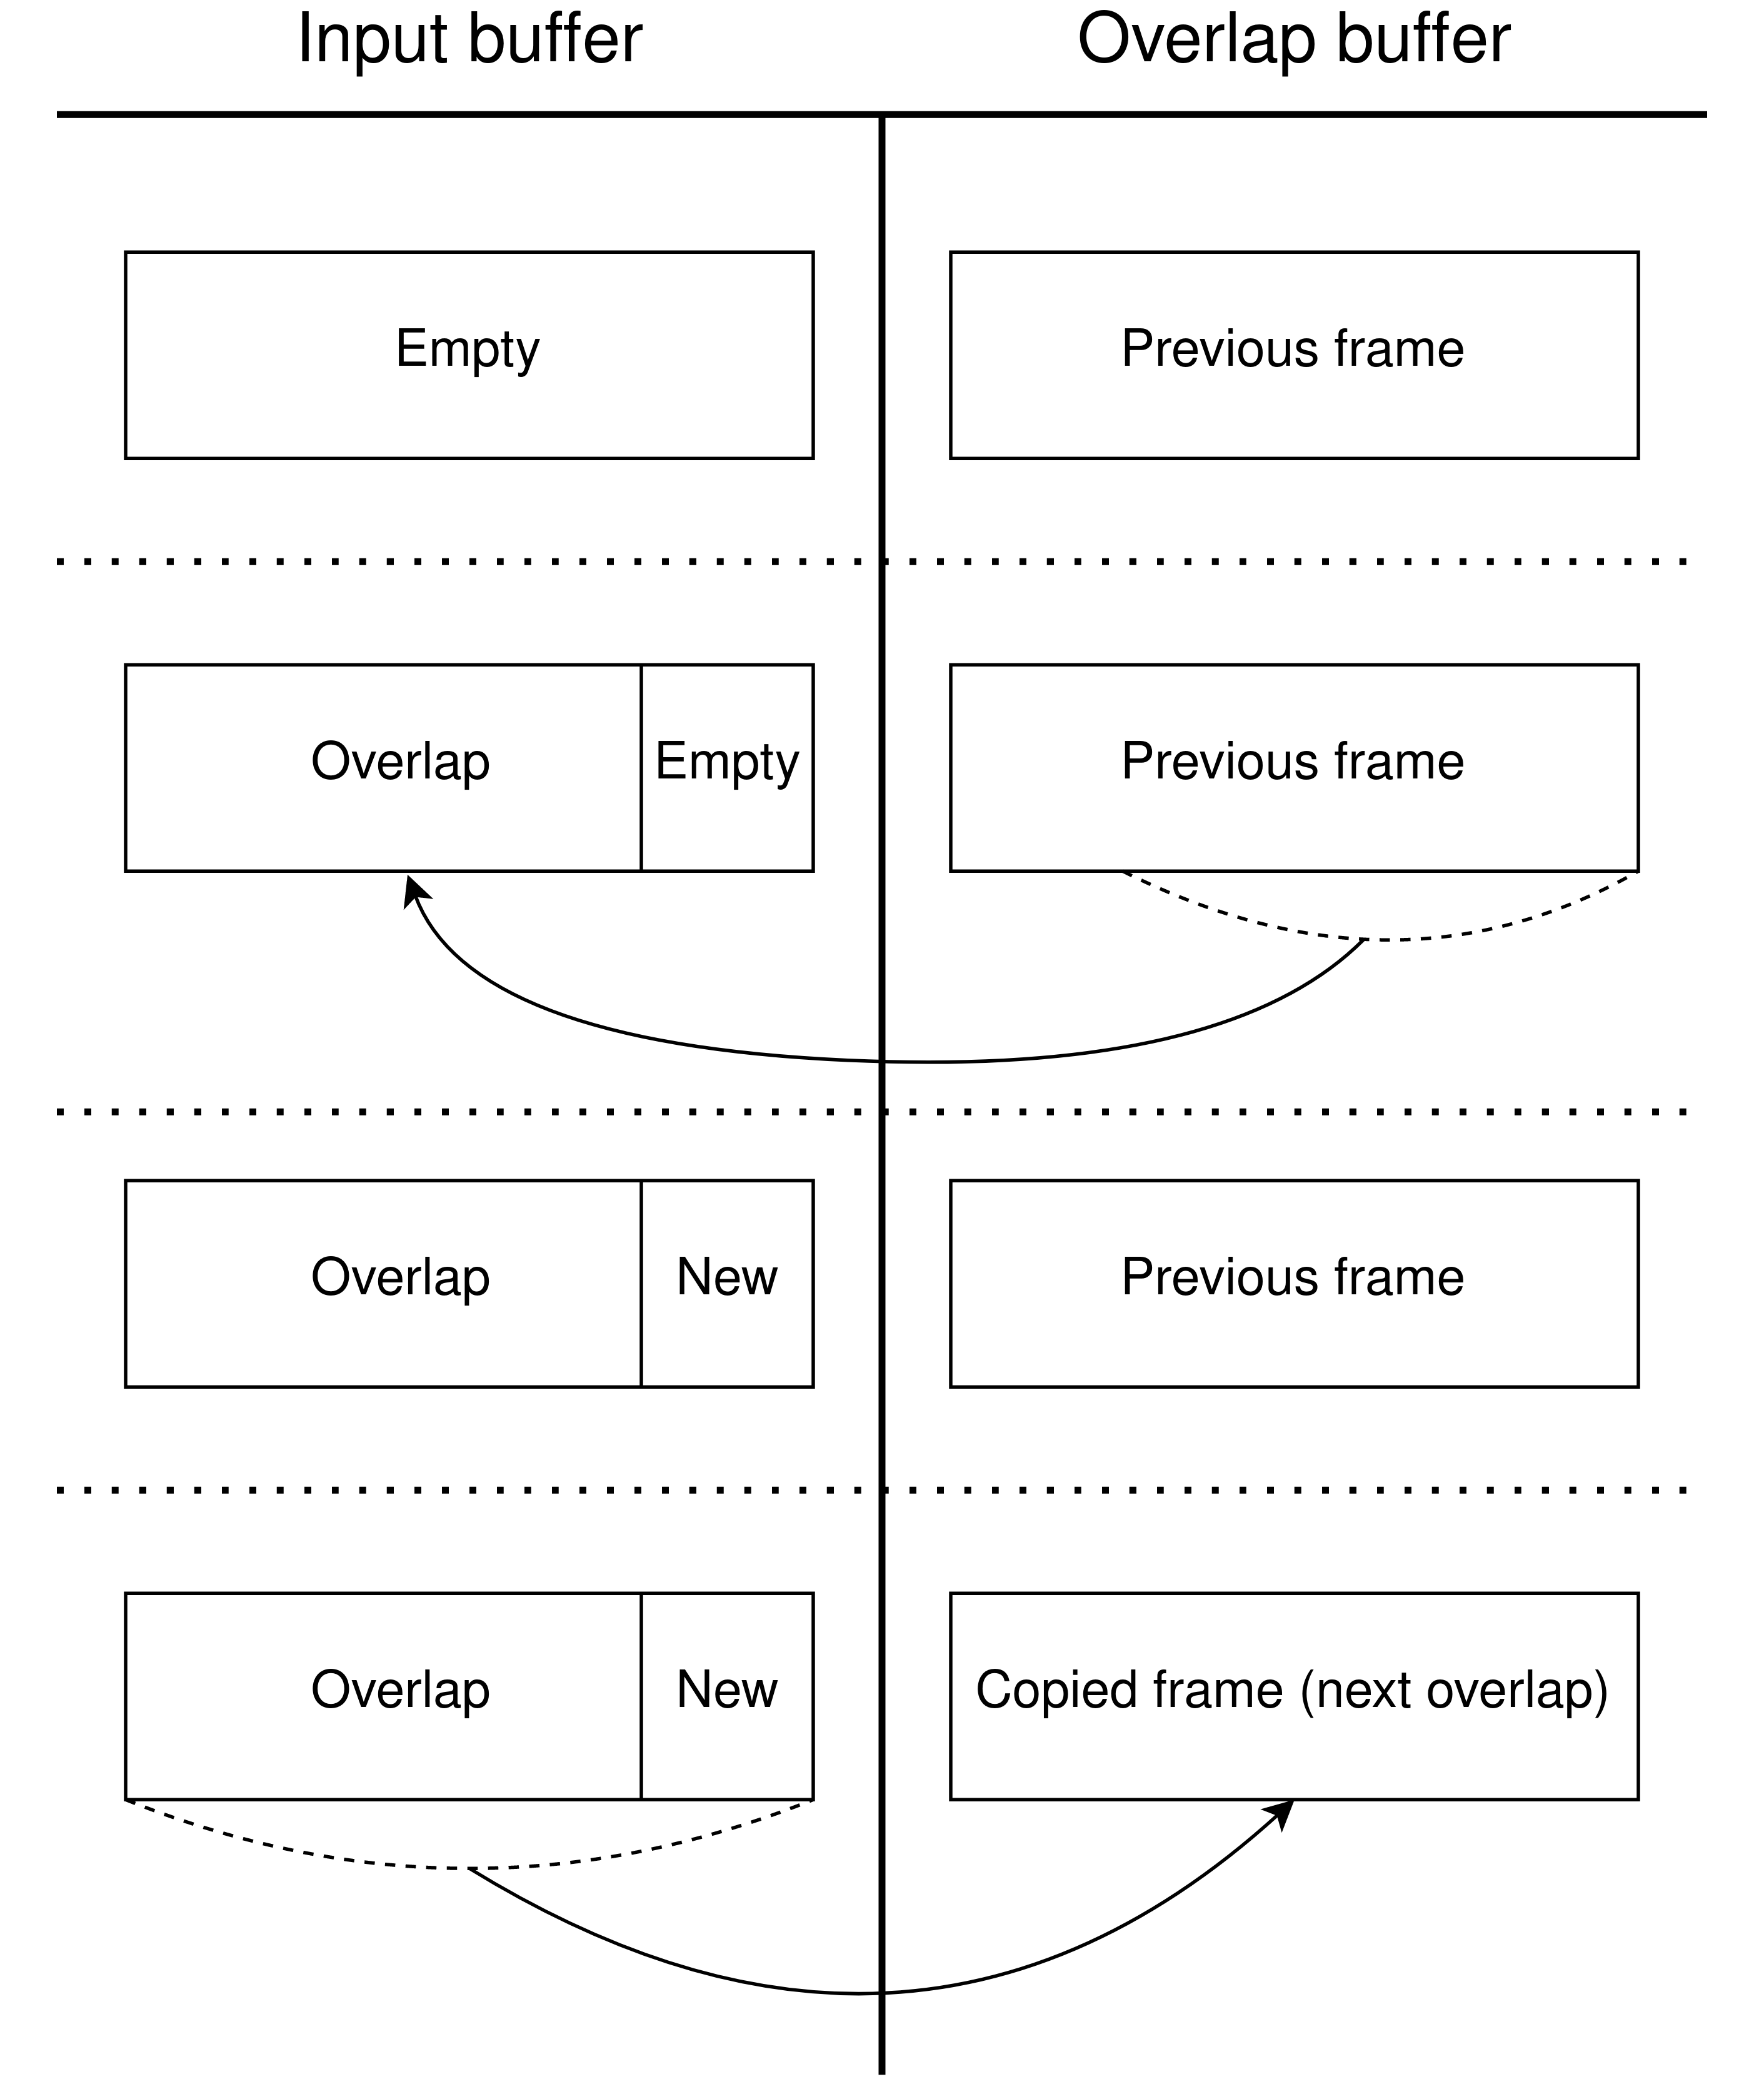
\includegraphics[width=0.9\linewidth]{fig/overlap3.png}
    \caption{Graphical overview of overlap copy-pasting. The sample getter start with an empty input buffer and the previous frame stored in the overlap buffer. First, we copy the relevant part of the overlap frame to the start of the input buffer. The rest of the input buffer is filled with new samples. Lastly, we copy the entire frame to the overlap buffer for the next get sample call.}
    \label{fig:overlapgraph}
\end{figure}

Since estimators are agnostic to overlapping, the note events reported by the estimator will overlap if the input frames overlap. Since the output modules assume every given note event list to directly follow the preceding one, we have to adjust the note events to only reflect the newly acquired samples. As a consequence, it is possible for an estimator to find a note in the beginning of a frame which was not found when the note was at the end of the frame. In other words, it may find a note event completely in the past which was not found when the relevant samples were the present. We discard these past note events, as past information is irrelevant in real time pitch estimation.

When reading samples from an audio device, there might not be enough samples ready to fill a frame. This might cause partial reads on non-blocking audio APIs, which are solved using a basic read loop. Here, we simply loop the read call until the frame is filled, which causes high CPU usage. However, using the sample rate, we can calculate how long we have to wait until enough samples are ready and sleep for this duration. This reduces the CPU usage of Digistring, which makes Digistring run more energy efficient\footnote{On an AMD 3700X using the parameters described in Section~\ref{sec:exp}, we measured a power consumption of 29 and 37 watt with and without the optimization respectively.}. However, this does require the operating system to guarantee a timely return from the sleep call, which in Linux is only the case when using the real-time kernel. Furthermore, modern CPUs scale down their performance when they are not fully utilized and it may take some time before the CPU is back in full performance mode, which causes additional latency after sleeping. As the optimization does not improve estimation accuracy or latency, we disabled it in Digistring.
% The difference in power consumption may be of significance when running Digistring on specialized hardware.

We have implemented four different sample getters in Digistring. The most important one is \texttt{audio\_in}, which retrieves samples from the audio driver. This sample getter allows us to play live with Digistring. For performing automated experiments and to aid with parameter fine tuning, we implemented \texttt{audio\_file}. Currently, it only supports reading from \texttt{.wav} files. We also implemented \texttt{sine\_generator} and \texttt{note\_generator}, which generate sine waves tuned to specific frequencies or notes respectively. These are useful for debugging and testing. %The generated frequency/note can be changed at runtime.
% For information about adding additional sample getters to Digistring, see Appendix~\ref{sec:add_to_digistring}.


\subsection{Real time sound synthesis}  \label{sub:rtsynth}
To verify if the results of an estimator are musically sound, we implemented a synthesizer interface in Digistring. Given a list of note events, a sample buffer and its size, the synthesizer will fill the buffer with samples such that, when played back, the resulting sound correctly represents the note events. Generating the samples has to be done carefully, as discontinuities in the generated samples may cause audible plops in the resulting audio.% This means we cannot generate sound waves in the buffer exactly where the note events describe them, as note events likely no not align with the wave's periods.

There are two cases where discontinuities may arise when synthesizing sine waves. The first is within a buffer. If we for example want to generate a one hertz sine wave for 1.25 seconds, the wave would end at its highest point and go back to silence the next sample, causing a large discontinuity. We can circumvent this by altering the sine wave in such a way that it does reach a zero crossing before stopping. For instance, we can keep generating samples until the waveform reaches a zero crossing, which causes temporal distortion in the synthesized sound. In the case of sine waves, this quantizes note lengths to half the frequency, as sine waves have two equally spaced zero crossings. We can also stop the sine wave early if the previous zero crossing is closer than the next. Using this technique, the worst case temporal distortion on a guitar would be 3 milliseconds, as the \note{E}{2} has a zero crossing every $ \frac{1000}{82.41} / 2 \approx 6 $ milliseconds. We can also alter the end of the sine wave to force the end to zero, by either amplitude modulating the end of the wave or by adding samples which quickly go back to zero. These methods cause spectral distortions. % \textcolor{gray}{(distortions in time)} \textcolor{gray}{(distortions in frequency)}

The second case where discontinuities may arise is when a note is not finished at the end of a frame. If the note ended and the next frame contains silence at the start, the signal should go back to 0 as described in the previous paragraph. If the note sustains or another note is played at the start of the next frame, the synthesizer has to continue the next note with the same phase. Because of this, a synthesizer needs some inter-frame communication.

We have implemented several sine synthesizers. They all share the same base algorithm. We first start by zeroing the synth buffer. Then, we try to finish sines which were not zero at the end of the previous frame. Lastly, we iterate over all note events and add the corresponding sines to the synth buffer. If any sines are not zero at the end of a frame, we add them to a list so that we can finish them next frame. An example of generating sine waves of a arbitrary frequency in a sample buffer given a certain sample rate can be seen in Algorithm~\ref{alg:xqifft_error} on Line~\ref{alg:xqifft_error:sinesynth}. Here, \textit{phase offset} and \textit{last phase} are used to make sure the sine in continuous between frames.

% \textcolor{gray}{TODO: Rewrite. }
% Our sine synthesizer algorithm starts by zeroing the synth buffer. We first try to zero notes which were not zero at the end of the previous frame. Then, we iterate over every note event and add the generated sine wave samples corresponding to the note event to the synth buffer in the right place. We make sure both ends of the note event samples are at zero by temporally shifting the offset of the note. We only shift the offset, as the onset is more important for conveying rhythm. For every note event that could not reach zero at the end of the synth buffer, we save the note and the phase corresponding to the last generated sample. By saving the phase of the last sample of a note, we can continue at the correct position in the corresponding sine wave in the next frame. This algorithm will always ensure continuity, even if there is polyphony in the note events.

% There is one small caveat with this algorithm in the polyphonic case. For instance, if we generate two overlapping sine waves of the same frequency, but one sine temporally shifted half a wavelength, the two waves will cancel each other out. If they are generated a full wavelength apart, they will amplify each other maximally and might cause clipping. Mixing multiple audio channels is out of the scope of this thesis, so we simply ignore this problem. In practice, these cases rarely show up.

% As mentioned in Section~\ref{sec:fourier}, accurate estimation of signal power is difficult. Instead, we rely on relative signal power estimation. .

% Currently, we have implemented \textcolor{red}{TODO synths}. %For information about adding additional synths to Digistring, see Appendix~\ref{sec:add_to_digistring}.


\subsection{Optimize XQIFFT exponent}  \label{sub:opt_xqfft}
As discussed in Section~\ref{sub:qifft}, when performing XQIFFT, we need to carefully choose the exponent with which to weight the bins. To test the error of XQIFFT for some exponent $\epsilon$, we generate many different sine waves and perform pitch estimation as we normally would. As we are transforming pure sines, we can pick the loudest bin as our estimated pitch. After finding this bin, we can XQIFFT the true peak location and return the found pitch. Since we know the original frequency of the generated sine, we can calculate a measure of error. For instance, we can minimize the mean error over all frequencies or minimize the maximum error. We chose to use the mean squared error for a combination of the two. See Algorithm~\ref{alg:xqifft_error} for an example of such an algorithm.

On line~\ref{alg:xqifft_error:freq}, we generate a sine for every cent in an octave starting at a low frequency. We chose this method because it focuses on lower frequencies, which need the most resolution. However, we empirically found that the exact series of frequencies does not influence the results significantly if enough sines are generated. Moreover, the error may vary slightly depending on the starting phase of the sine. To prevent a bias, we generate multiple sine waves of different phase for every frequency, causing the phase error of average out.
\input{pseudo_code/xqifft_error.pc}
\input{pseudo_code/optimize_xqifft.pc}

As error increases for exponents further away from the optimum, we can iteratively approximate the optimal exponent. See Algorithm~\ref{alg:optimize_xqifft} for a pseudo-code implementation of such an algorithm. Here, we start our search at some arbitrary range. Then, we calculate the error of some points in this range. These points can be calculated in parallel for an enormous speed-up. If the minimum value is at either end of the range, we have to search further in that direction. We always overlap two points with neighboring ranges, in case the end of the range is the minimum value for that search resolution. Otherwise, we update the search range to the two values surrounding the minimum point and repeat the optimization process.


\subsection{Experimentation and estimation feedback tools}  \label{sub:tools}
As mentioned in the intro of this section, good experimentation and estimation feedback tools are necessary in order to build a well performing real-time pitch estimation system.

Experiments in AMT rely on datasets containing sound files accompanied with annotation files describing the notes present in the sound files. This means that in order to experiment on a pitch estimation system, we need to be able to feed the sound files to the pitch estimation system and compare its results to the annotations. The former is possible through the \texttt{audio\_in} sample getter. To allow for the latter, Digistring can write its estimations results to a JSON formatted file.

To compare the Digistring results to annotations, we created a Python tool called \textit{generate report}. Given a Digistring output file and the corresponding dataset annotation, it can calculate many different performance measures. Furthermore, it can generate plots which visualize the annotations and pitch estimation results in a MIDI piano roll like fashion; see Figure~\ref{fig:dat3} for an example.
% \begin{figure}[h]
%     \centering
%     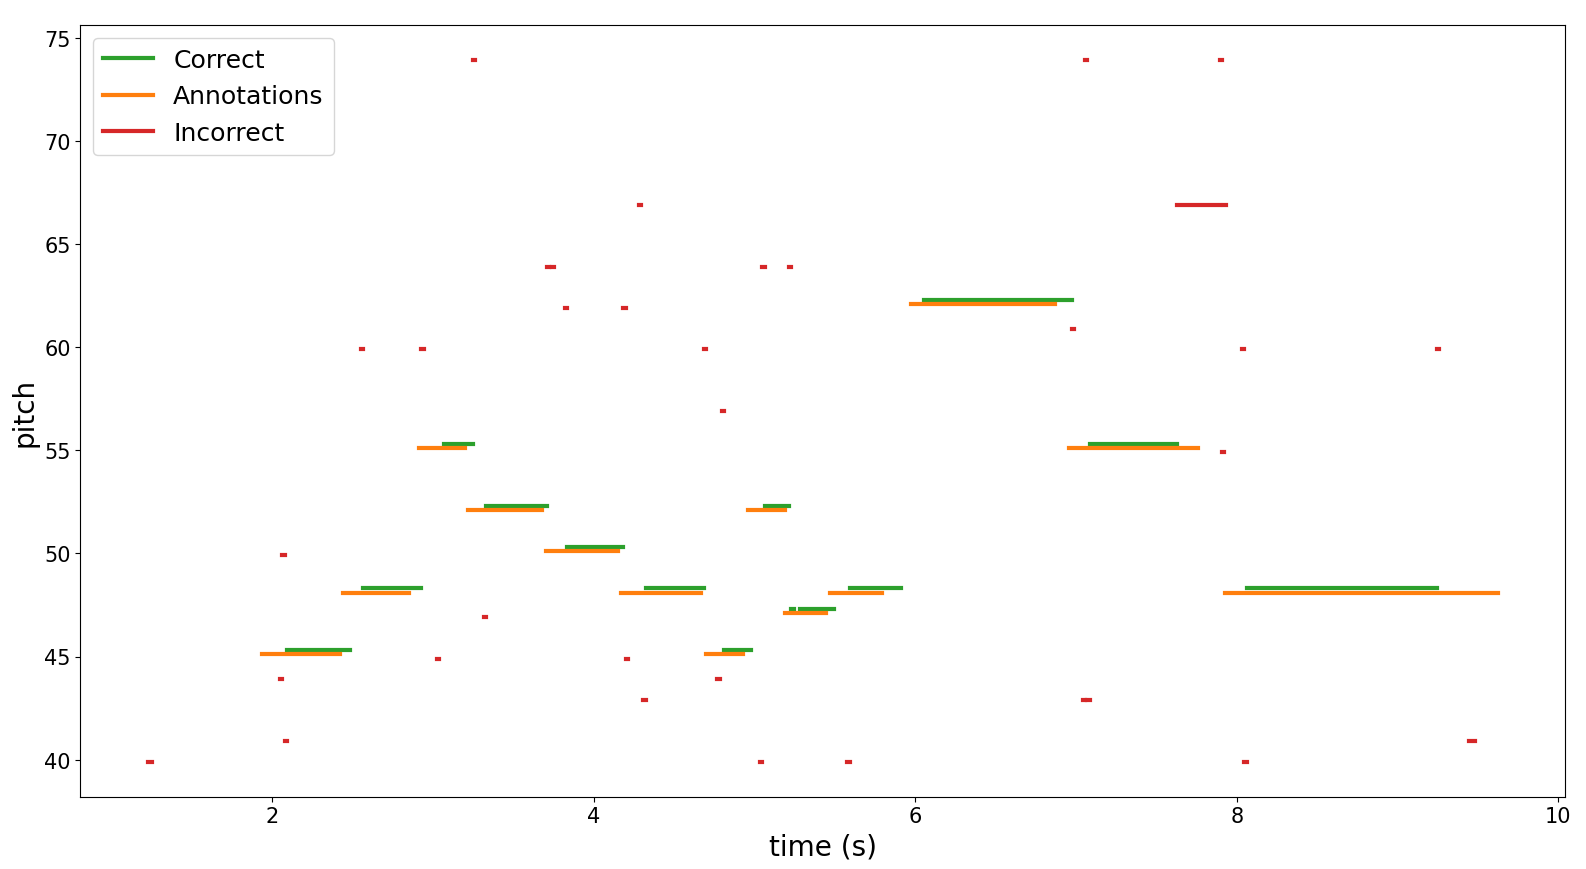
\includegraphics[width=\linewidth]{fig/generate_report.png}
%     \caption{\textcolor{gray}{TODO: Better image.} TODO: Caption.}
%     \label{fig:pianoroll}
% \end{figure}
Unfortunately, every dataset uses its own annotation standard. Because of this, we parse the annotation file into an intermediate representation. This allows us to use the tool for different datasets by solely implementing a parser for the annotation standard. Furthermore, the Digistring output is also parsed into this intermediate representation, which means this tool can also be used with different estimation systems by writing a parser for the estimation system's output. The different performance measures are then calculated from this intermediate representation.

In order to visualize the pitch estimation process, we allow Estimators to define an EstimatorGraphics object, which holds information regarding the last processed frame. This information can be rendered using visualizers. For instance, we can render the spectrum as a spectrogram or waterfall plot, or plot the raw input waveform; see Figure~\ref{fig:screens} for examples. The spectrogram visualizer can also render signal envelopes and found peaks, which allows us to precisely fine-tune parameters regarding these.
\begin{figure}[p!]
    \centering
    \begin{subfigure}{\linewidth}
        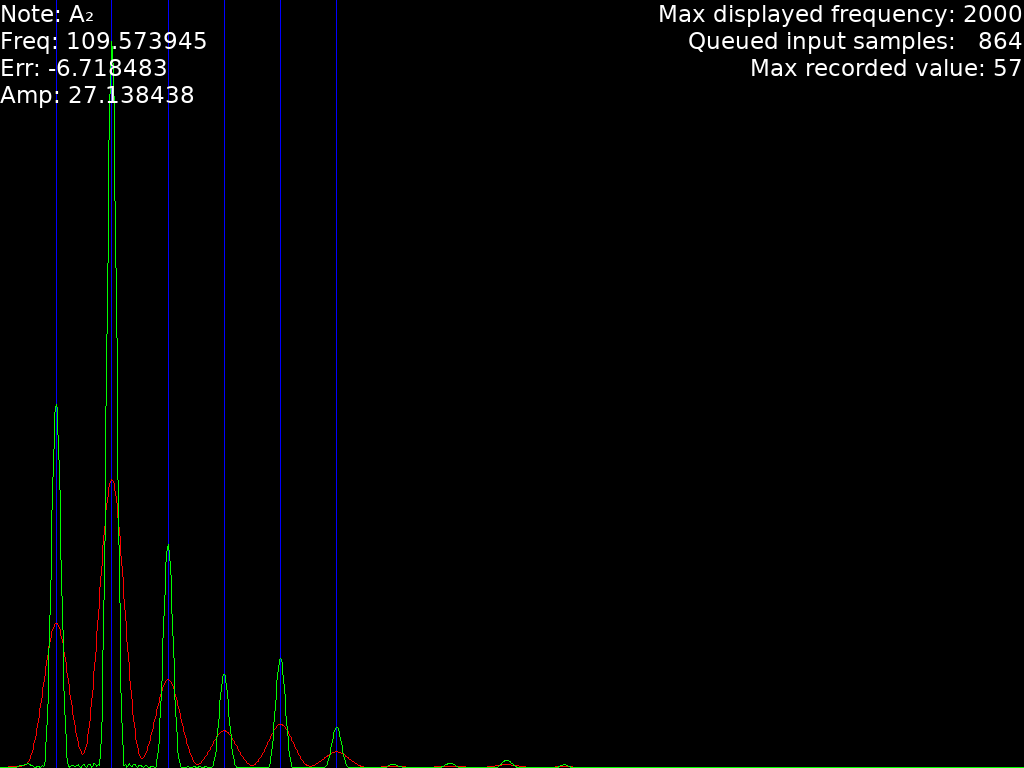
\includegraphics[width=\linewidth]{fig/digi_spec.png}
    %     \caption{}
    \end{subfigure}
    \begin{subfigure}{\linewidth}
        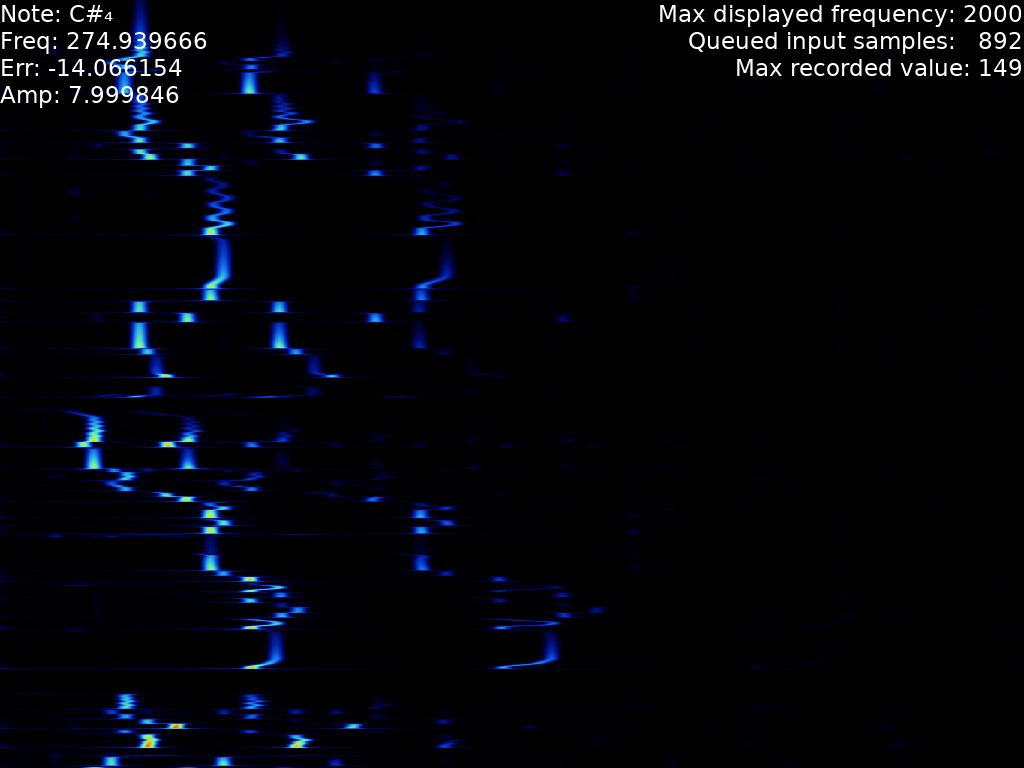
\includegraphics[width=\linewidth]{fig/digi_water.png}
    %     \caption{}
    \end{subfigure}
    \begin{subfigure}{\linewidth}
        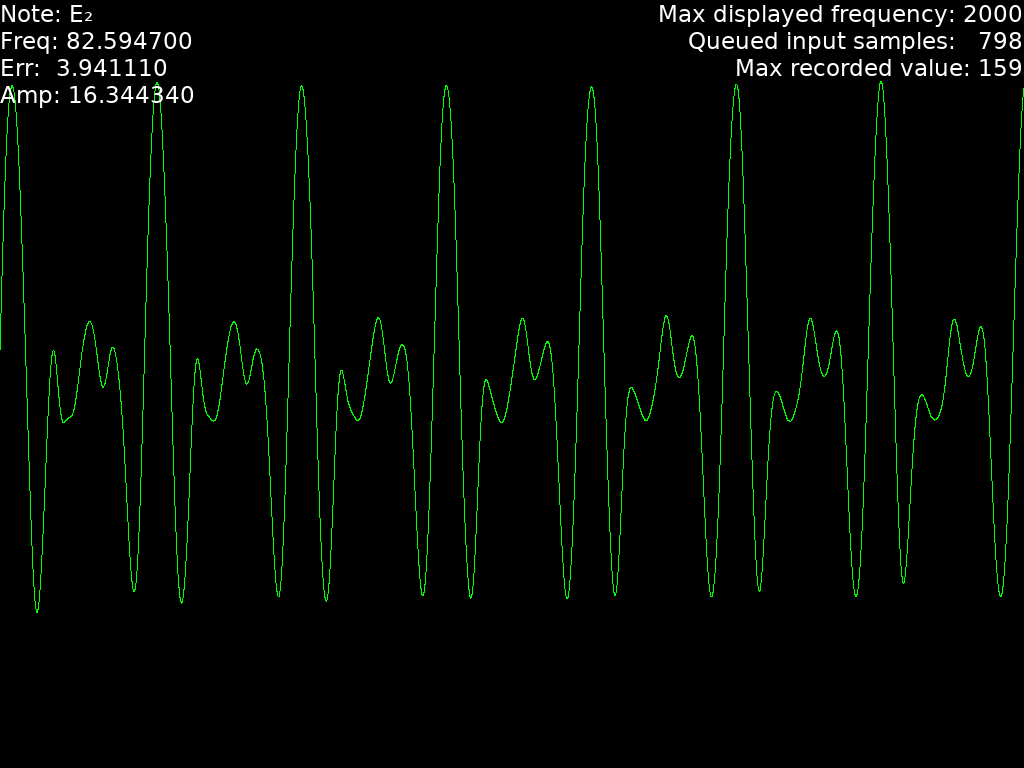
\includegraphics[width=\linewidth]{fig/digi_wave.png}
    %     \caption{}
    \end{subfigure}
    % \caption{Screenshots of different graphing modes of Digistring.}
    \caption{Screenshots of different graphing modes of Digistring. The top image show the spectrogram plotter. Here, the spectrum is displayed in green, the Gaussian envelope in red and the selected peaks in blue. The middle image shows the waterfall plotter. These plots move downward through time and show the spectrum on the horizontal axis. Brighter colors equate to higher amplitudes. On the bottom is the signal plotter, which displays the raw time domain signal.}
    \label{fig:screens}
\end{figure}
\begin{table*}[b!]
    \centering
    \begin{tabular}{c|ccc}
        Method & mean squared error & mean error & max error \\
        \hline
        Nearest bin & 0.178952 & 0.366332 & 0.731592 \\
        MQIFFT & 0.0493383 & 0.198229 & 0.318431 \\
        LQIFFT with $\ln$ & 0.0200228 & 0.12687 & 0.242515 \\
        LQIFFT with $\log_2$ & 0.0200228 & 0.12687 & 0.242515 \\
        LQIFFT with $\log_{10}$ & 0.0200228 & 0.12687 & 0.242515 \\
        dB-QIFFT ($20 * \log_{10}$) & 0.0200228 & 0.12687 & 0.242515 \\
        XQIFFT ($\epsilon = -0.301939$) & \textbf{0.0173085} & 0.114302 & 0.41559 \\
        XQIFFT ($\epsilon = -0.764585$) & 0.0233141 & \textbf{0.107375} & 0.603697 \\
        XQIFFT ($\epsilon = 0.0554724$) & 0.0210592 & 0.129826 & \textbf{0.212814}
    \end{tabular}
    \caption{Overview of interpolation errors in hertz using different interpolation methods. For the XQIFFT methods, we tested three values for $\epsilon$. The first minimizes mean squared error, the second minimizes mean error and the last minimizes max error.}
    \label{tab:qifft_error}
\end{table*}

As we focus on real-time pitch estimation, we need to be able to measure the run-time performance of different parts of the system. This is possible through our performance measuring class, which allows us to set labelled measurement points in the code between which elapsed time is measured. The measured times are written to a file which can be interpreted by our \textit{performance plot} tool, which can visually show the distribution of run-times for each time point; see Figure~\ref{fig:plotspeed} for an example of such a plot. Using this information, we can see which processes introduces the most latency to our pitch estimation system.
% \vfill\pagebreak

To better understand the estimation process during transients, we implemented a slowdown mode. This stretches the note events reported by the estimator, effectively slowing down the estimation process, which in turn can slow Digistring down. This allows us to better find filters which can suppress note estimations during transients.

As mentioned in Section~\ref{sub:rtsynth}, synthesizers are an important tool in verifying the musical correctness of estimated note events. To better verify the synthesized result matched the input signal, we allow for the input signal and synthesized signal to be played back simultaneously split over the two stereo channels. Furthermore, it is also possible for Digistring to output MIDI events, which allows Digistring to be used with existing MIDI synthesizers.

% \subsection{Playback latency}  \label{sub:playback_latency}
% \textcolor{gray}{Details on how we made the playback latency tool.}

% As mentioned in Section~\ref{sec:constraint}, the critical latency is an important measure when setting a real-time constraint. To aid in determining the critical latency, we developed \textit{delayed playback}. This tool plays back incoming audio with an arbitrary latency.



\section{Experiments}  \label{sec:exp}
In order to assess the performance of our pitch estimation system, we perform a few experiments. First, we measure the error of the different QIFFT methods so we can choose the best method for our pitch estimation system. Then we will try to assess a lower limit on latency using Fourier based pitch estimation methods on a guitar to test if Fourier based methods can ever be feasible. Subsequently, we will run some speed tests on our pitch estimation algorithm to see if our real-time goal is met. Then, we have an in depth discussion on using Digistring as a guitar synthesizer. Lastly, in order to obtain some quantitative measure on the over all pitch estimation performance, we run the Fraunhofer dataset~\cite{datasetproc, dataset} through Digistring.

% The different parameters which control the pitch estimation process were empirically optimized. There is still room from improvement through parameter tuning, however, as the accuracy and latency would only marginally improve, we opted to safe us the time. At best, we can save a few milliseconds and filter some noisy estimations from transients.

The different parameters which control the pitch estimation process were empirically optimized. We used the following parameters for all experiments, unless otherwise is stated. The frame size is 8192 samples with a sampling rate of 192000 Hz. This coincides with a frame time of 42.67 ms and a Fourier bin size of 23.44 Hz. We zero-pad the buffer 15 times, resulting in an actual frame size of 131072 samples, giving us a interpolated bin size of 1.46 Hz. The overlap factor is set to 0.85. The minimum signal power is set to 15 and the envelope threshold is set to 0.25. Gaussian peak-picking uses a sigma of 1.25 and a kernel width factor of 0.0005. The signal to noise factor is set to 0.05. The range filter matches the range of a guitar, which is between \note{E}{2} and \note{E}{6}.


\vfill
\subsection{QIFFT errors}  \label{sub:exp:qifft}
To help choosing the best QIFFT strategy, we measured the performance of the different strategies using the method outlined in Section~\ref{sub:opt_xqfft}. The results are listed in Table~\ref{tab:qifft_error}. The bin size during these tests was approximately 1.465 Hz. The nearest bin method coincides with no interpolation. As a consequence, the worst error is equal to half the bin size and the average error is equal to half the worst error.

We can see that LQIFFT significantly reduces the error compared to nearest bin and MQIFFT. Furthermore, all LQIFFT methods perform the same, invariant to logarithm base or linear scaling factor. Lastly, we can see that XQIFFT only situationally outperforms LQIFFT. In general, no value of $\epsilon$ strictly outperforms LQIFFT. Because of this, we opted not to use XQIFFT. Note that the error reduction of XQIFFT compared to LQIFFT is significant if no zero-padding is used.
\begin{figure*}[b!]
    \centering
    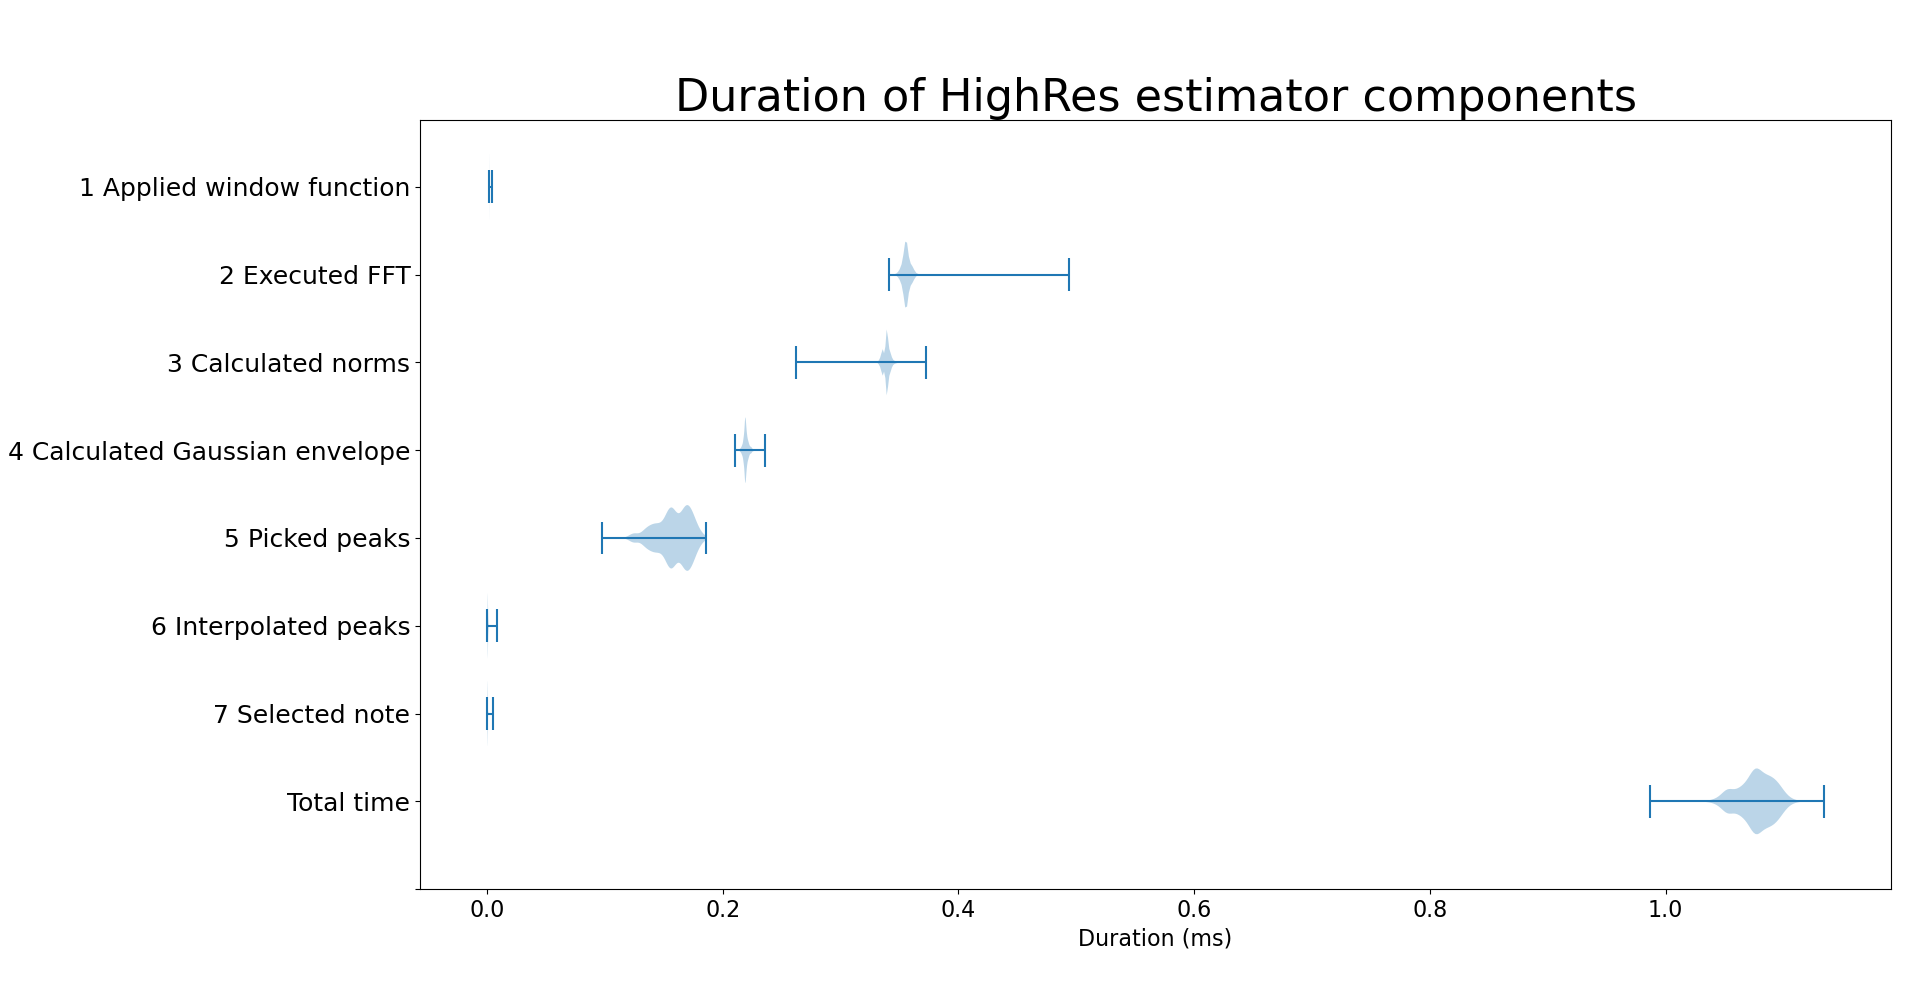
\includegraphics[width=\linewidth]{fig/perfplot3.png}
    \caption{Plots of distribution of run times for every HighRes estimator component.} %The bottom plot is the top plot zoomed in.
    \label{fig:plotspeed}
\end{figure*}
\pagebreak


\subsection{Fourier frame size limit}
The limiting factor for low latency Fourier based pitch estimation is the size of the transformed frame. The size of the frame determines the lowest two notes we can discern. Therefore, given we need to be able to discern the \note{E}{2} and the \note{F}{2}, we can find the limit on minimum frame size our pitch estimation system needs.

We start with discerning pure sine waves to get an estimate on the theoretical lower limit of our pitch estimation method. Here, we found that we can reliably discern \note{E}{2} and \note{F}{2} with a frame size of 1024 samples with 15 times zero-padding for a total frame size of 16384. This equates to a frame length of 5.33 ms.

To get a more practical lower limit, we did the same test on recordings of \note{E}{2} and \note{F}{2} played on a guitar. Here, we found we need 5760 samples for consistent results, equating to a frame length of 30 ms. Note that even though we can reliably discern \note{E}{2} and \note{F}{2} at this frame size, the measured frequencies are dissonant. This means we cannot use the obtained frequency information for note synthesis, only the note information, implying we can only synthesize tuned notes from the results.
% Here, we found that at a frame size of 4096, the spectrum behaved to chaotically to find a consistent peak for any of the two notes. Moreover, the fundamental frequency and the first overtone often become one lobe. At a frame size of 8192, we can get very reliable results.
\vfill\pagebreak

\subsection{Pitch estimation speed}  \label{sub:expspeed}
As we are performing pitch estimation in real-time, the speed of the process is very important. We measured the execution time of our algorithm running on an AMD 3700X CPU. Figure~\ref{fig:plotspeed} shows the distribution of execution times of the different parts of the pitch estimation process. Here, we can see the processing time of a frame is insignificant compared to the length of the frame.

% To speed up calculating the Gaussian envelope, we can parallelize computing each envelope point. On average, we measured a 10 times speed-up over the sequential version. However, the parallel version suffers from 

On average, it takes the HighRes estimator 1.1 ms to process a frame of 42.7 ms. This means our estimator runs 38.8 times real-time. In other words, our pitch estimation algorithm can process samples 38.8 faster than it acquires them. The total latency of our pitch estimation algorithm is 43.8 ms.


\subsection{Performance discussion}  \label{sub:watvindik}
Unfortunately, it is almost impossible to capture the performance of our pitch estimation system quantitatively. Some errors might completely ruin the results, while others might not matter at all. Furthermore, certain guitar techniques do not work well in guitar driven synthesis. Because of this, we will try to discuss the performance of Digistring as a guitar synthesizer.% from a guitarists perspective.

First should be noted that using a guitar synthesizer should be viewed as playing a different instrument similar to a guitar. It will be very familiar to a guitarist, but directly playing songs as one would normally play them will cause bad results. Most importantly, one should try to play as clean as possible. This means strumming the notes carefully to prevent string to overdrive and keep transients at a minimum. Furthermore, all unused strings should be thoroughly muted. Palm muting slightly reduces the power of transient, however, it also impacts the sustain of played notes.

The main problem for our pitch estimator is transients. This means techniques such as shredding and double picking do not work well. Moreover, pull-offs and hammer-ons work well, as they barely cause transients. Our pitch estimator is very sensitive to small amplitude signals, which makes tapping much easier. Moreover, it allows to play the guitar in a piano like fashion, where both hands tap notes on the fretboard, much easier.

Our estimator support bending. However, this does require the synthesizer to be able to generate tones between notes, which is often not the case for piano synthesizers.

Given the above information, we can conclude guitar solos generally work very well for our pitch estimation algorithm. They are very melodic and often carefully played. In contrast, metal performs very bad in our pitch estimator. Metal often conveys fast rhythms through guitar, which end up as a big mess of transients to our estimator. Furthermore, metal is often played on the lowest notes of a guitar, which are the most difficult for our estimator.

Unfortunately, we were not able to remain within our real-time constraint of 20 milliseconds. The critical latency is however highly subjective. Out of five users, one user did not notice the latency until we brought it up, while two users deemed it too high for real-time usage. The other two did notice the latency, but had no problems with it. We found that after playing for a while, you get used to the latency and found it not to be too problematic. The impact of the latency is also largely dependent on synthesizer used to generate the audio. When using a synthesizer with a slow attack, the swell effectively masks the latency.

We recorded some examples of Digistring during live usage. Videos of this can be found on \url{github.com/lucmans/digistring-demo}. Here, we also provide the raw guitar input, which can be run through Digistring to generate the content from the videos yourself.


\subsection{Pitch estimation accuracy}
In order to obtain a quantitative measure on Digistring's performance, we run a subset of the Fraunhofer dataset~\cite{dataset} through Digistring. The Fraunhofer dataset contains both monophonic and polyphonic recordings. As our pitch estimation algorithm is monophonic, we will only use the monophonic recordings in the dataset. The dataset is split into four different subsets. Three of the subsets contain monophonic recordings, with a total of 350 monophonic recordings. The dataset is recorded at a sample rate of 44100 Hz, so we have to change the frame size and Gaussian kernel width factor to 1882 and 0.002 respectively.

% Unfortunately, the recording quality of the dataset is not the best. Notes often distort slightly and are not always fretted cleanly. These mistakes cause problems for our estimator. As the dataset consists of raw guitar output, the recording artists were likely listening to the raw feedback. This often causes guitarists play too loud to compensate for not having any amplification, causing distortions and other effects from unnatural guitar play.
The dataset is challenging for our HighRes pitch estimator. As mentioned in Section~\ref{sub:watvindik}, playing using our estimator is slightly different from playing guitar normally. In the dataset, notes often overdrive slightly and are not always fretted cleanly. This is not a problem for normal guitar play, however, it causes problems for our estimator. As a consequence, the measurements reflect Digistring's performance on normal guitar play instead of Digistring's performance as a guitar synthesizer.
% As discussed in the previous section, a guitar driven synthesizer should almost be considered a different instrument from a guitar. 

The first subset consists of 312 single note recordings. Each recording contains one note. There is a recording of the open string along with all fretted notes to the 12th fret for every string. There are four versions. Three use the same Ibanez guitar with different pick-up configurations (neck/bridge) and one uses a Fender guitar. For each version, we measured if the note was correctly identified, if at least 90\% of the annotated event was found and if we found one uninterrupted note event. The results are summarized in Table~\ref{tab:expacc}. Here, we can see all notes were correctly identified. Unfortunately, many notes are not identified as one continuous note event due to small distortions in the recordings.
\begin{table}[b]
    \centering
    \begin{tabular}{r|rrr}
        version     & correct & $t_{>0.9}$ correct & no interrupt \\
        \hline
        Fender      & 100 \%  & 96 \%   & 81 \% \\
        Ibanez N    & 100 \%  & 96 \%   & 76 \% \\
        Ibanez B    & 100 \%  & 87 \%   & 51 \% \\
        Ibanez N+B  & 100 \%  & 92 \%   & 67 \%
    \end{tabular}
    \caption{Results of the first subset of the Fraunhofer dataset. 'Correct' shows if the correct note was estimated at all, '$t_{>0.9}$ correct' shows if at least 90\% of the estimated frames were the correct note and 'no interrupt' shows if recording was estimated as one note event.}
    \label{tab:expacc}
\end{table}

Interestingly, we can see significantly better results from the neck pick-up compared to the bridge pick-up on the Ibanez guitar. We could not replicate these results with any of our guitars, including an Ibanez guitar. We found no notable difference in pitch estimation accuracy between different pick-ups. The difference we found in the dataset is likely from the inconsistent playing quality between recordings.

The second subset consists of six licks played on three different guitars. Every lick is played with a plectrum and finger style, resulting in a total of 36 recordings. 
% Unfortunately, the licks are played a bit rash, resulting in much guitar noise in the recordings. In turn, it causes many transient errors. 
The results are summarized in Table~\ref{tab:expacc2}. Here, we can see we did not miss any notes, however, due to the earlier mentioned playing style, we often do not find the full note. We can see a significant difference between finger style playing and playing with a pick. When we tried to replicate these results, we only found a small difference between the two playing styles. The large difference is likely because licks written to be played with a pick are often difficult to play finger style. We found that playing finger style may lead to smaller transients, but more inconsistent overtone behavior due to the dampening from soft finger skin.
\begin{table}[h]
    \centering
    \begin{tabular}{r|rr}
        version          & correct & $t_{>0.8}$ correct \\
        \hline
        Fender pick      & 100 \%  & 83 \% \\
        Fender finger    & 100 \%  & 58 \% \\
        Gibson pick      & 100 \%  & 75 \% \\
        Gibson finger    & 100 \%  & 58 \% \\
        Aristides pick   & 100 \%  & 79 \% \\
        Aristides finger & 100 \%  & 63 \%
        % total            & 100 \%  & 69 \%
    \end{tabular}
    % \\\vspace{+2mm}~\\
    % \begin{tabular}{r|rrr}
    %     version          & P & R & F1 \\
    %     \hline
    %     Fender pick      &  &  &  \\
    %     Fender finger    &  &  &  \\
    %     Gibson pick      &  &  &  \\
    %     Gibson finger    &  &  &  \\
    %     Aristides pick   &  &  &  \\
    %     Aristides finger &  &  &  \\
    %     total            & 0.20 & 1.0 & 0.34
    % \end{tabular}
    \caption{Results of the second subset of the Fraunhofer dataset.}
    \label{tab:expacc2}
\end{table}

The last subset consists of five small excerpts of famous classical pieces, of which only two are monophonic. The estimation overview is shown in Figure~\ref{fig:dat3}. Here, we can see all notes were correctly identified. In promenade, we can see the end of the first note is missing, however, this is a mistake in the annotations. Even though it is a monophonic recording, we can see the second note overlapping the first note in the annotations. Other than that, the only errors are transient errors. The transient errors are of small amplitude, so are barely audible when using them for note synthesis.
\begin{figure*}[!p]
    \centering
    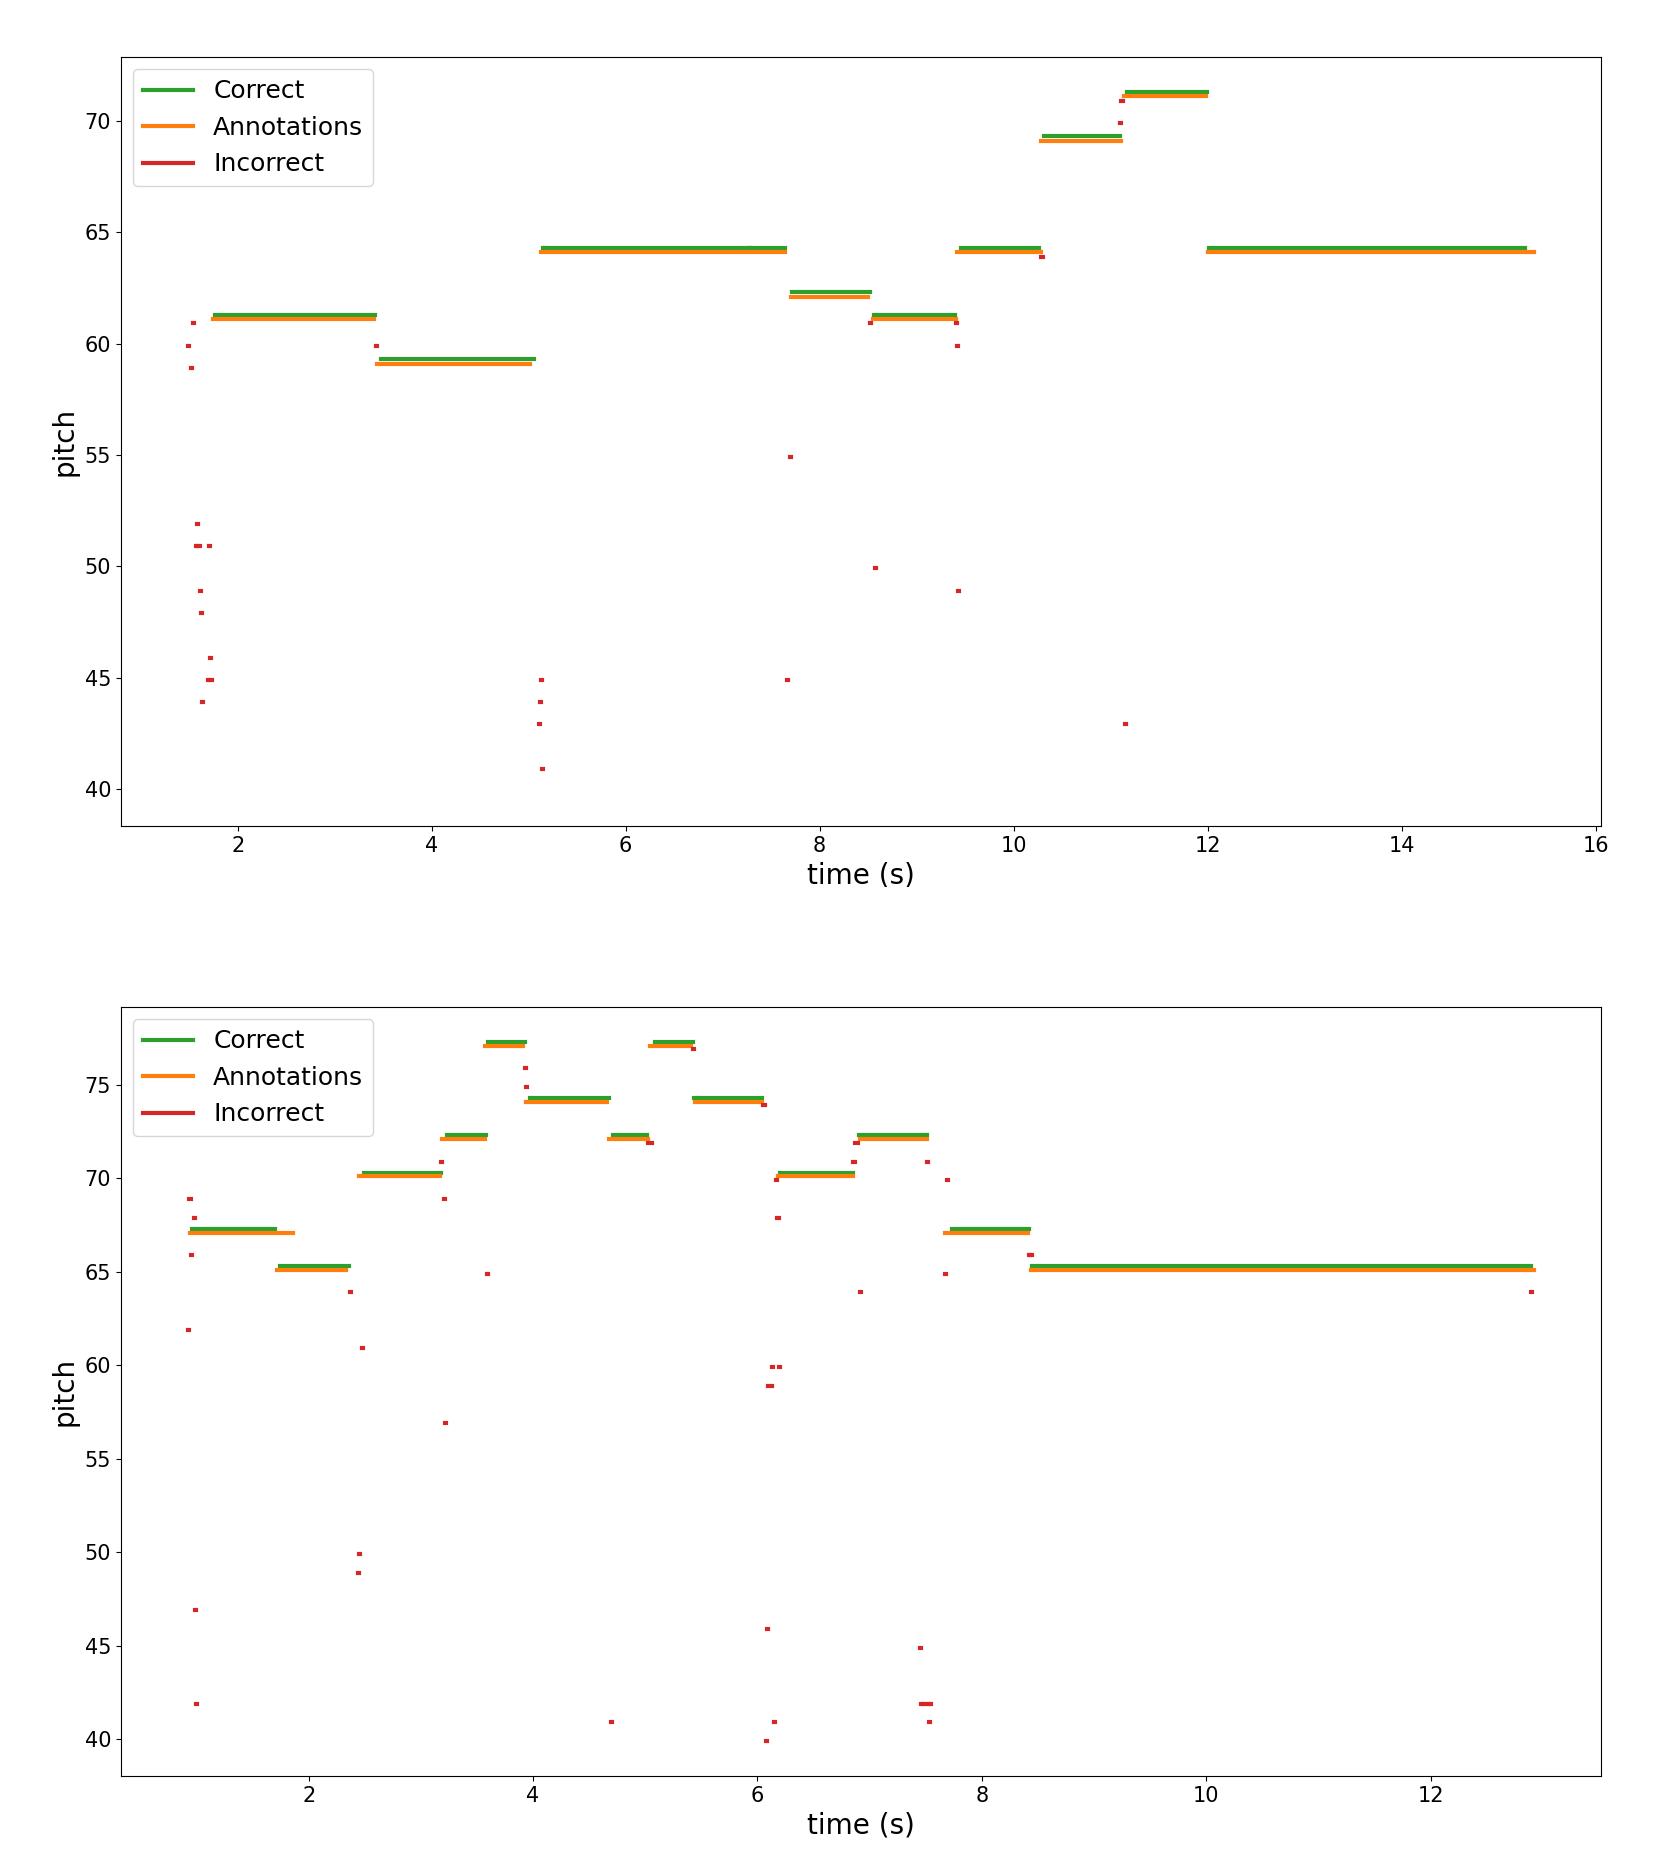
\includegraphics[width=\linewidth]{fig/dataset3.png}
    \caption{Results of the third subset of the Fraunhofer dataset. The top and bottom image show the pitch estimation results for Pathetique and Promenade respectively.}
    \label{fig:dat3}
\end{figure*}



\section{Conclusions}
In this thesis, we constructed a Fourier transform based real-time pitch estimation algorithm. We found the limiting factor of such systems is the fundamental trade-off between frame length and frequency resolution. In order to have enough frequency resolution to discern the two lowest notes on a guitar, the \note{E}{2} and \note{F}{2}, we would need a frame length of 200 milliseconds for an frequency resolution of 4.9 Hz. This exceeds our real-time constraint of 20 milliseconds by a significant amount. Through interpolation, we can reduce the frame length. We found we can reduce it to 43 milliseconds using zero-padding and LQIFFT, which equates to a frequency resolution of 23.44 Hz. When we only focus on note estimation in contrast to exact frequency estimation, we can further reduce the frame length to 30 milliseconds. Unfortunately, this is still over our real-time constraint. We could adhere to our real-time constraint if choose a higher lowest note.

To reduce the frame length, we looked at XQIFFT~\cite{interpolnozero}, as the paper shows an 100 to 1000 times reduction in interpolation error. However, we found our that this large error reduction is only possible when no zero-padding is used. With our level of zero-padding, XQIFFT only situationally outperforms LQIFFT.

% During performance analysis, we found that calculating the Gaussian envelope of the signal takes a significant amount of time. The main advantages of Gaussian peak picking are related to polyphonic transcription. As such, we should look to replace the peak picking strategy for a faster one. However, this can only improve our latency by 2.5 milliseconds at best, which is not enough difference to achieve our real-time goal.

Through our experiments, we found our pitch estimator can reliably estimate the correct pitch if a note persists for long enough. However, during the transient of a note, we still produce random estimations. We could better filter these random estimations, however, we found that a prolonged silence at the onset played worse than having the wrong transient estimations. Furthermore, the estimations from transients are often of low amplitude, causing synthesized audio to only softly play the transient errors. Even though our estimator exceeds our real-time constraint, it is still fast enough to play with. It should be noted that the critical latency is highly subjective and as such, some people who tried Digistring did not notice the latency, while others found it a deal-breaker. When using synthesizers with a slow attack, the latency and transient errors are no problem at all, as by the time the synthesized audio is in full volume, the note estimation has already stabilized.



\section{Future work}  \label{sec:future}
There is still much to improve on the HighRes estimator. However, the current estimation strategy likely cannot ever function within our real-time constraint for the full range of a guitar due to fundamental limits of the Fourier transform.

Our pitch estimation algorithm discards the phase information provided by the Fourier transform. However, we can use the phase estimation to refine the frequency estimation~\cite{phaseinfo}. If we know the phase of a specific frequency and the hop size between two frames, we can extrapolate what the phase should be in the next frame. The error of this estimate compared to the measured phase of the next frame can be used to refine the frequency estimation.

While analyzing the raw guitar signal, we found that the waveform consists of "packets", see Figure~\ref{fig:osc_overview} for an example. These packets form, among other things, because of the fundamental frequency which suppresses the waveform close to its zero-crossing. Autocorrelation pitch estimation methods work well because these packets look alike. However, the first packet which occurs during the transient differs. As a consequence, autocorrelation might slightly misjudge the distance between the first two packets and estimate the wrong note.

For future research, we would look into accurately calculating the distance between the first two packets. The time between these packets is equal to the inverse of the frequency. When analyzing the signal from an \note{E}{2} in an oscilloscope, we found the second packet finished 15 milliseconds after onset. This gives us 5 milliseconds of headroom for pitch estimation to remain within our real-time constraint. Packet based methods are likely less stable than Fourier based methods, as small errors in packet distance measurements will quickly cause an entirely different note to be estimated. We would suggest combining both methods by using packet based methods for fast estimations and Fourier based methods for slow stable estimations.

% TODO: Note tracking.



\appendix
\vspace{+4mm}
\section{Measuring the latency of the AXON AX 100 mkII}  \label{sec:ax100}
To compare our work to commercial guitar to MIDI solutions, we performed some experiments on the Axon AX 100 mkII. Many thanks to Elgar van der Zande for letting us use his lab equipment and helping with the experiments.

For our first experiment, we tried to trigger pitch estimation by sending a pure sine wave to the Axon using a signal generator. Surprisingly, this led to an error on the Axon. Changing the type of waveform or frequency had no effect. Only after generating at least two overtones does the Axon produce a pitch estimation. This shows us that the existence of overtones is very important to the Axon's pitch estimation system.

Next, we set out to determine the pitch estimation latency of the Axon. To do so, we connected both the guitar input to and MIDI output from the Axon to an oscilloscope. We also connected the audio output of the Axon to measure the synthesizer latency. %For the MIDI output, we could simply connect a probe to the correct pin on the 5-pin DIN connector, however, 
Then, if we set the oscilloscope to trigger on any MIDI signal change, we can take the difference between that time point and the start of the guitar signal. An example of the images the oscilloscope produces can be seen in Figure~\ref{fig:osc_overview}.
\begin{figure}[t]
    \centering
    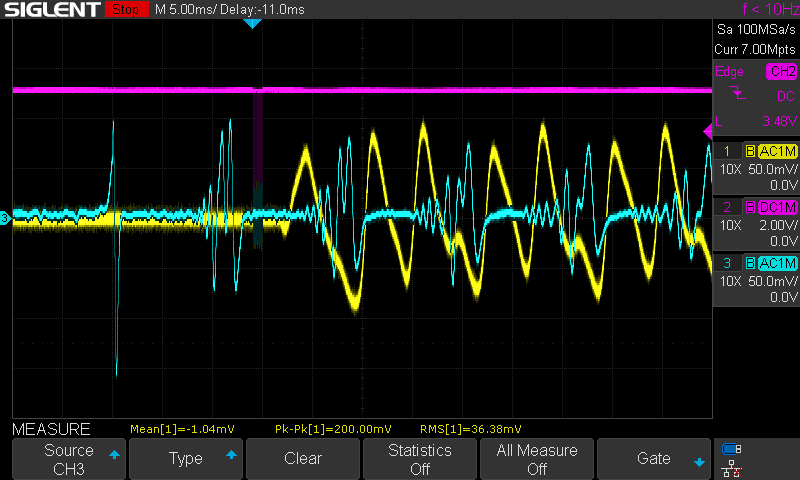
\includegraphics[width=\linewidth]{fig/osc_1.png}
    \caption{Example of measurement on an oscilloscope. Here, the blue line is the analog guitar input, the purple line is the MIDI output and the yellow line is the synthesized audio output. In this image, we played an \note{E}{2}. The blue triangle on top shows us where the oscilloscope triggered on the MIDI signal. Then, using the distance between this and the start of the blue waveform, we can determine the pitch estimation latency.}
    \label{fig:osc_overview}
\end{figure}
\begin{table}[t]
    \centering
    \begin{tabular}{c|ccc}
        String-fret & normal & 12th & 6th \\
        \hline
        E0  & 15.8 & 34.1 - 38.8 & 30.5 - 38.9 \\
        E1  & 14.8 & 30.9 - 37.2 & 29.3 \\
        E12 & 12.9 - 13.6 & - & - \\
        G0  & 12.5 & 15.1 & 14.6 \\
        G1  & 13.3 & 14.6 & 13.8 \\
        G12 & 12.4 & - & - \\
        e0  & 11.0 & 11.1 & 12.0 \\
        e1  & 11.9 - 12.5 & 11.6 - 12.4 & 11.0 - 12.5 \\
        e12 & 12.2 & - & -
    \end{tabular}
    \caption{Latency between receiving a guitar signal and outputting a MIDI signal in milliseconds. E refers to the low pitched E string and e refers to the high pitched E string.}
    \label{tab:osc_results}
\end{table}

For both E strings and the G string, we measured the latency while playing the open string, the first fret and the twelfth fret. Every note was played using a plectrum at the normal picking position. For the open string and first fret measurements, we also picked each note at the twelfth fret and sixth fret. Every measurement was performed three times. The measurements are summerized in Table~\ref{tab:osc_results}. Here, we can see the Axon has significantly higher latencies on low pitched notes. This is exacerbated when strumming the note further up the neck. Moreover, during our experimentation, we noticed that the Axon either had a quick estimation between 11 and 15 milliseconds, or a slow estimation between 25-40 milliseconds. This may indicate there are two estimation algorithms at work. When the quick one is not confident enough, the result of the slower algorithm is awaited.

% Note that latencies ascertained from the oscilloscope images might not reflect the playing latency. There might be a small latency between strumming a note and generating a waveform. For instance, at the start of strumming a note, the string is only displaced, not resulting in sound. Then, when the pick slides off the string and the string is released to vibrate freely, the resulting waveform can start to exist.

Lastly, we checked the pitch estimation latency when feeding the Axon pure sine signals from a signal generator. Here, we feed the Axon with a signal consisting of a sine wave along with three overtones on the input for the low pitched E string. See Table~\ref{tab:osc_siggen} for an overview of the results. The latencies for 65.4 Hz and 440 Hz were surprisingly high, where the two frequencies close to E0 (\note{E}{2} in scientific notation) performed similar to the guitar signal. This may indicate that the Axon only outputs note estimations that are generally in range of a string, or it has to be very sure of the estimation result.
\begin{table}[h]
    \centering
    \begin{tabular}{c|c}
        $f_0$ & latency (ms) \\
        \hline
        65.4 & 48.4 \\
        82   & 15.68 \\
        82.4 & 15.8 \\
        440  & 74.8
    \end{tabular}
    \caption{Latency of pitch estimation when using a generated sine signal with additional 3 overtones.}
    \label{tab:osc_siggen}
\end{table}



% \section{Effect of different window functions}  \label{sec:windows}
% \textcolor{gray}{Plots met effect van verschillende window functions. Rectangular narrowest main lobe and least ENBW. The Hann window is an all round performing window and as a result is often used. The Welch window is a window with a very narrow center lobe. The Dolph–Chebyshev window has little and very evenly spread overall leakage (optimal filter). Parzen window (and b-spline windows per extension) have much space between lobes (lobe density).}
% for ENBW of different windows: https://www.gaussianwaves.com/2020/09/equivalent-noise-bandwidth-enbw-of-window-functions/

% \begin{figure}[h]
%     \centering
%     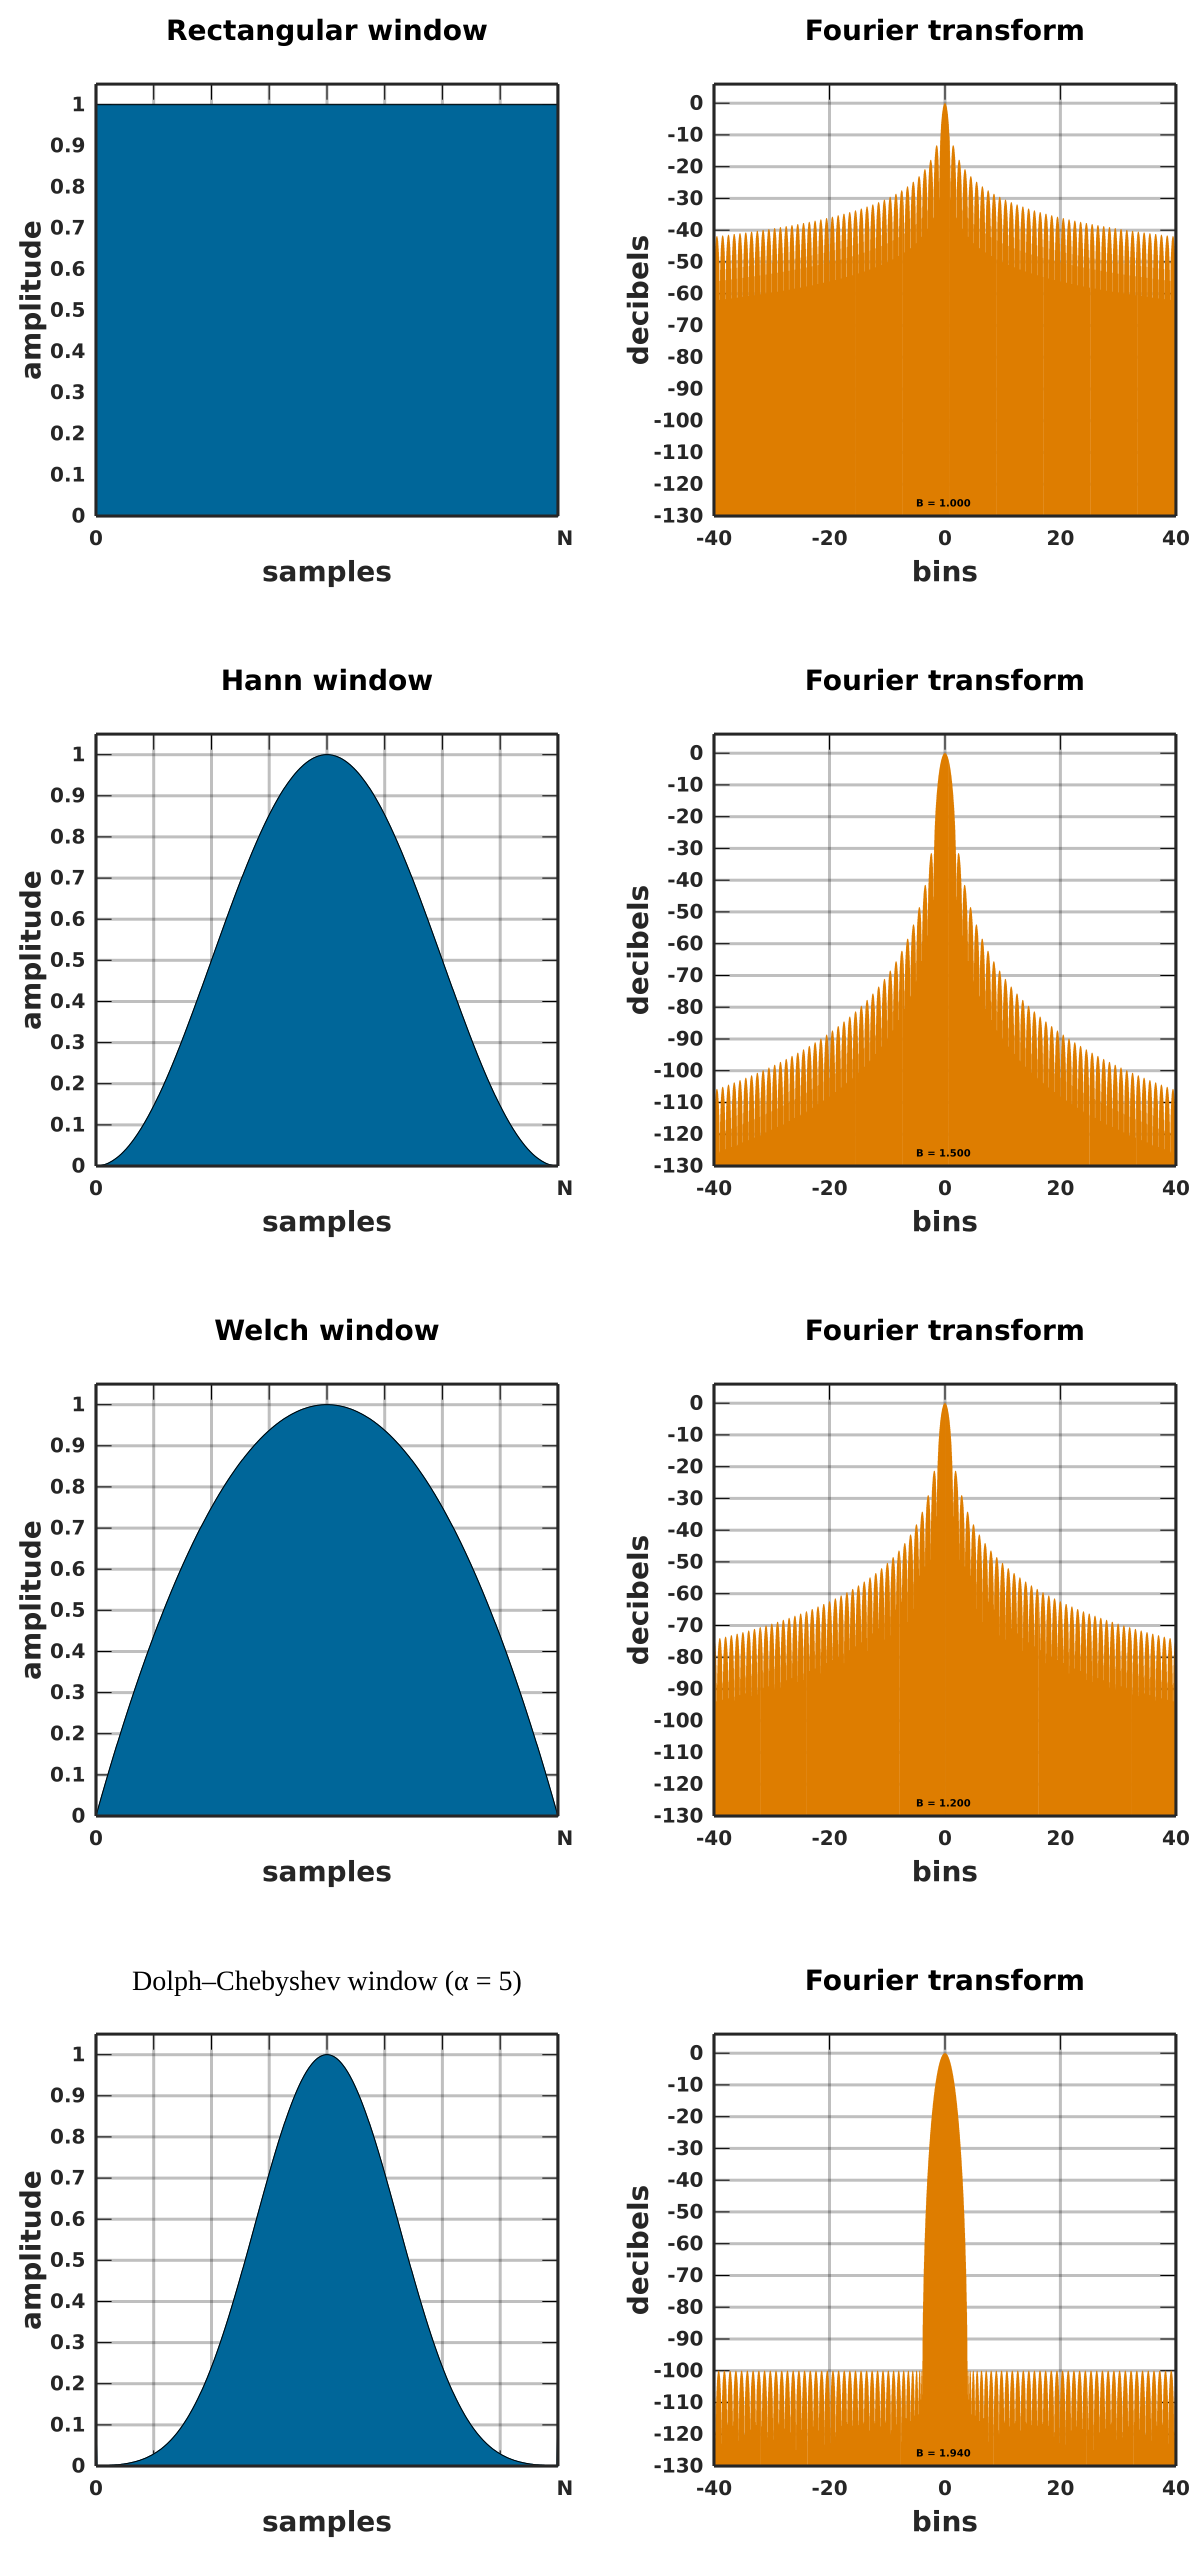
\includegraphics[width=\linewidth]{fig/windows.png}
%     % 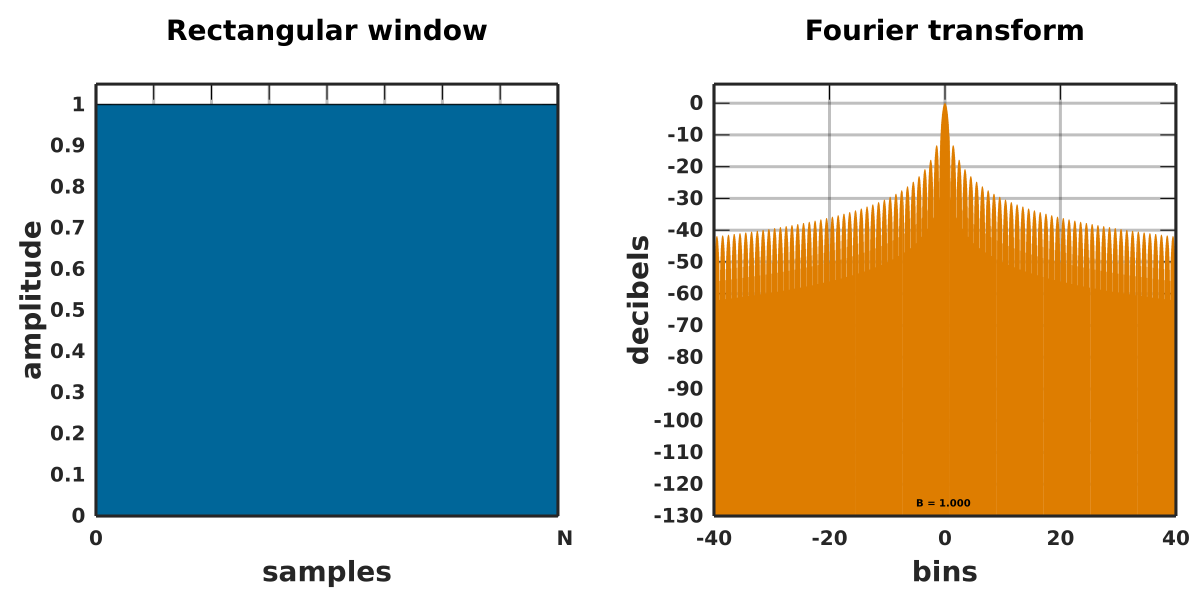
\includegraphics[width=\linewidth]{fig/window_rect.png}
%     % 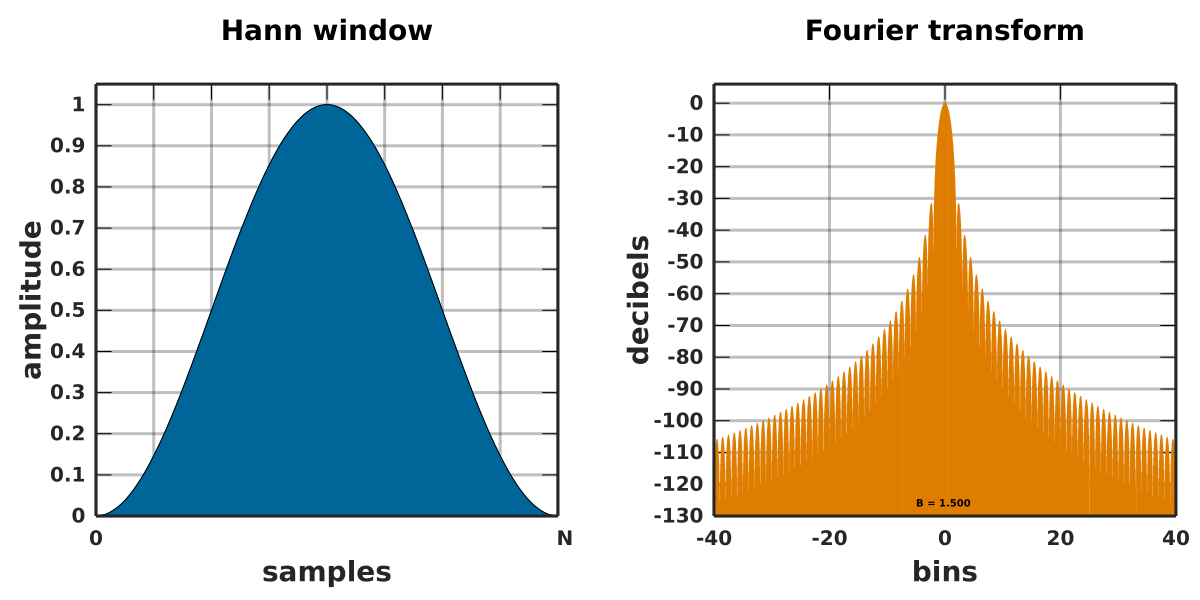
\includegraphics[width=\linewidth]{fig/window_hann.png}
%     % 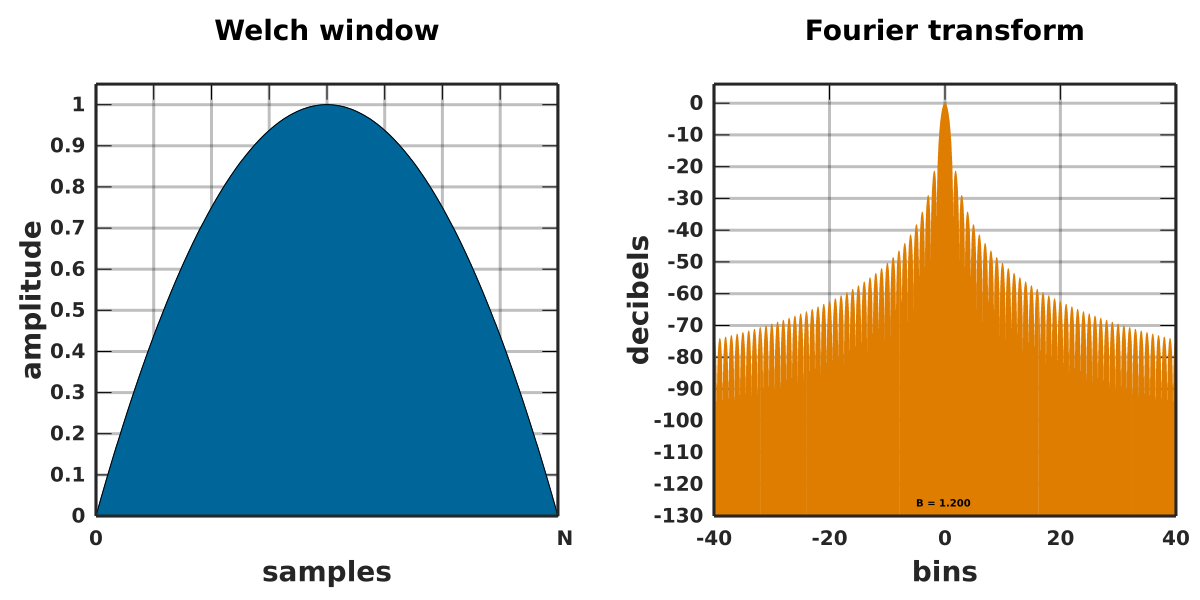
\includegraphics[width=\linewidth]{fig/window_welch.png}
%     % 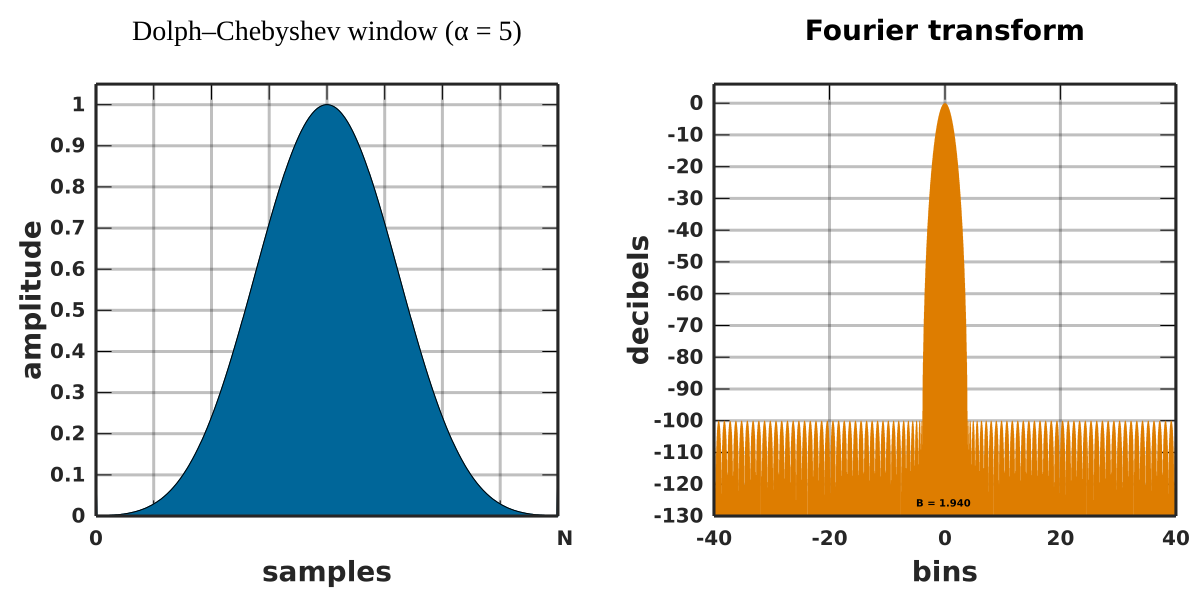
\includegraphics[width=\linewidth]{fig/window_dolph.png}
%     \caption{Examples of the spectral leakage of some window functions.}
%     \label{fig:windowfunceffect}
% \end{figure}



% \section{Extending Digistring}  \label{sec:add_to_digistring}
% \textcolor{gray}{Title: Expanding Digistring?}
% One of the main goals of Digistring is extendability. This allows people researching pitch estimation or real time sound synthesis to use Digistring as a basis. Currently, there is an interface to add sample getters, estimator along with estimator graphics and synthesizers.


% \subsection{Adding a sample getter}
% TODO


% \subsection{Adding an estimator with estimator graphics}
% TODO


% \subsection{Adding a synthesizer}
% TODO



\addcontentsline{toc}{section}{Bibliography}

\begin{thebibliography}{XX}
\bibitem{hearing}
Zhiyao Duan, Bryan Pardo and Changshui Zhang. Multiple Fundamental Frequency Estimation by Modeling Spectral Peaks and Non-Peak Regions. \textit{IEEE Transactions on Audio, Speech, and Language Processing}, 18(8):2121--2133. 2010.

\bibitem{nopoly}
Eric J. Anderson. Limitations of Short-Time Fourier Transforms in Polyphonic Pitch Recognition. Ph.D. qualifying project report. \textit{University of Washington, Department of Computer Science and Engineering}. 1997.

\bibitem{perception}
Michael J. O'Donnell. Digital Sound Modeling: Perceptual Foundations of Sound. Lecture notes. \textit{University of Chicago}. 1994, 2004 revision.\\
\url{http://people.cs.uchicago.edu/~odonnell/Scholar/Work_in_progress/Digital_Sound_Modelling/lectnotes/node4.html}\\
Last accessed on 04-10-2021

\bibitem{isoa}
ISO 16:1975. Acoustics — Standard tuning frequency (Standard musical pitch). \textit{International Organization for Standardization}. 1975.

\bibitem{ik}
Luc de Jonckheere. Real-time guitar transcription using Fourier transform based methods; A pitch estimation framework and overtone sieve algorithm. \textit{Leiden University}. 2021.

\bibitem{monotopoly}
Fabrizio Argenti, Paolo Nesi and Gianni Pantaleo. Musical Robots and Interactive Multimodal Systems. Automatic Music Transcription: From Monophonic to Polyphonic, pages 27--46. \textit{Springer Berlin Heidelberg}. 2011.

\bibitem{overtones}
R. S. Shankland and J. W. Coltman. The Departure of the Overtones of a Vibrating Wire From a True Harmonic Series. \textit{The Journal of the Acoustical Society of America}, 10(3):161 ff. 1939.

\bibitem{timbre}
Kristoffer Jensen. Timbre Models of Musical Sounds. PhD thesis, University of Copenhagen. 2021.

\bibitem{realclass}
Hermann Kopetz. Real-Time Systems: Design Principles for Distributed Embedded Applications. \textit{Springer US}. 1997.

\bibitem{windowfunc}
F.J. Harris. On the use of windows for harmonic analysis with the discrete Fourier transform. \textit{Proceedings of the IEEE}, 66(1):51--83. 1978.

\bibitem{interpolgaus}
M. Gasior and J. L. Gonzalez. Improving FFT Frequency Measurement Resolution by Parabolic and Gaussian Spectrum Interpolation. \textit{AIP Conference Proceedings}, 732(1):276--285. 2004.

\bibitem{zeropad1}
Meinard Müller. Fundamentals of Music Processing. \textit{Springer Cham}. 2015.
% Webpage with interactive tool that shows the effect of zero-padding.\\
% \url{https://jackschaedler.github.io/circles-sines-signals/zeropadding.html}\\
% Last accessed on 20-10-2021

% \bibitem{zeropad2}
% Webpage on the limits of zero-padding.\\
% \url{https://dspillustrations.com/pages/posts/misc/spectral-leakage-zero-padding-and-frequency-resolution.html#Frequency-Resolution}\\
% Last accessed on 20-10-2021

\bibitem{interpolnozero}
Kurt James Werner. The XQIFFT: Increasing the Accuracy of Quadratic Interpolation of Spectral Peaks via Exponential Magnitude Spectrum Weighting. \textit{Proceedings of the International Computer Music Conference}, pages 326--333. 2015

\bibitem{fourierlimit}
Eric J. Anderson. Limitations of Short-Time Fourier Transforms in Polyphonic Pitch Recognition. \textit{Technical report, Department of Computer Science and Engineering, University of Washington}. 1997.

\bibitem{sloomboi}
T. A. Goodman and I. Batten. Real-Time Polyphonic Pitch Detection on Acoustic Musical Signals. \textit{2018 IEEE International Symposium on Signal Processing and Information Technology (ISSPIT)}, pages 1--6. 2018.

\bibitem{sloomboi2}
Xander Fiss. Real-Time Software Electric Guitar Audio Transcription. \textit{Rochester Institute of Technology}. 2011.

\bibitem{oslatency}
Matthew Wright, Ryan J. Cassidy and Michael F. Zbyszyński. Audio and Gesture Latency Measurements on Linux and OSX. \textit{In Proceedings of the ICMC}, pages 423--429. 2004.

\bibitem{survey}
Tiago Fernandes Tavares, Jayme Garcia Arnal Barbedo, Romis Attux and Amauri Lopes. Survey on automatic transcription of music. \textit{Journal of the Brazilian Computer Society}, 19:589--604. 2013.

\bibitem{survey2}
Anssi Klapuri and Manuel Davy. Signal Processing Methods for Music Transcription. \textit{Springer}. 2006.
% Mads Græsbøll Christensen, Petre Stoica, Andreas Jakobsson and Søren Holdt Jensen. Multi-pitch estimation. \textit{Signal Processing}, 88(4):972--983. 2008.

\bibitem{CREPE}
J. W. Kim, J. Salamon, P. Li and J. P. Bello. CREPE: A Convolutional Representation for Pitch Estimation. \textit{2018 IEEE International Conference on Acoustics, Speech and Signal Processing (ICASSP)}, pages 161--165. 2018.

\bibitem{SPICE}
B. Gfeller, C. Frank, D. Roblek, M. Sharifi, M. Tagliasacchi and M. Velimirović. SPICE: Self-Supervised Pitch Estimation. \textit{IEEE/ACM Transactions on Audio, Speech, and Language Processing}, 28:1118--1128. 2020.

\bibitem{SWIPE}
Arturo Camacho and John G. Harris. A sawtooth waveform inspired pitch estimator for speech and music. \textit{The Journal of the Acoustical Society of America}, 124(3):1638--1652. 2008.


\bibitem{cqtalign}
Robert Dobre and Cristian Negrescu. Automatic music transcription software based on constant Q transform. \textit{8th International Conference on Electronics, Computers and Artificial Intelligence (ECAI)}, pages 1--4. 2016.

\bibitem{cqtfft}
Judith Brown and Miller Puckette. An efficient algorithm for the calculation of a constant Q transform. \textit{Journal of the Acoustical Society of America}, 92:2698--2701. 1992.

\bibitem{cqtslow}
Christian Schörkhuber and Anssi Klapuri. Constant-Q transform toolbox for music processing. \textit{Proc. 7th Sound and Music Computing Conf.}. 2010.

\bibitem{cqtres}
Gino Angelo Velasco, Nicki Holighaus, Monika Doerfler and Thomas Grill. Constructing an invertible constant-Q transform with nonstationary Gabor frames. \textit{Proceedings of the 14th International Conference on Digital Audio Effects, DAFx 2011}. 2011.

\bibitem{oud}
James A. Moorer. On the Transcription of Musical Sound by Computer. \textit{Computer Music Journal}, 1(4):32--38. 1977.

\bibitem{doublefourier}
K.A. Akant, R. Pande and S.S. Limaye. Accurate Monophonic Pitch Tracking Algorithm for QBH and Microtone Research. \textit{The Pacific Journal of Science and Technology}, 11(2):342--352. 2010.

\bibitem{octave}
A. Schutz and D. Slock. Periodic signal modeling for the octave problem in music transcription. \textit{In Proceedings of the 16th International Conference on Digital Signal Processing (DSP’09)}, pages 1--6. 2009.

\bibitem{numrec}
William H. Press, Saul A. Teukolsky, William T. Vetterling and Brian P. Flannery. Numerical Recipes: The Art of Scientific Computing. \textit{Cambridge University Press}. 1986.

\bibitem{ieeefloat}
IEEE 754-2008 - IEEE Standard for Floating-Point Arithmetics. 2018.%\\
% \url{https://ieeexplore.ieee.org/document/4610935}

\bibitem{dspfloat}
Steven W. Smith. The Scientist and Engineer's Guide to Digital Signal Processing. \textit{California Technical Publishing}. 2018.

\bibitem{presonus}
Y. Wang, R. Stables and J. Reiss. Audio Latency Measurement for Desktop Operating Systems with Onboard Soundcards. \textit{Journal of the Audio Engineering Society}. 2010.

% \bibitem{windowperf}
% Mathuranathan Viswanathan. Window function – figure of merits. \textit{GaussianWaves}. 2020.\\
% \url{https://www.gaussianwaves.com/2020/09/window-function-figure-of-merits/}\\
% Last accessed on 13-05-2022

\bibitem{windowperf2}
Stefan Scholl. Exact Signal Measurements using FFT Analysis. \textit{Microelectronic Systems Design Research Group}. TU Kaiserslautern. 2016.

\bibitem{windowperf3}
Wang Hongwei. Evaluation of Various Window Functions using Multi-Instrument. \textit{Virtins Technology}. 2021.

\bibitem{overlap}
G. Heinzel, A. Rudiger and R. Schilling. Spectrum and spectral density estimation by the Discrete Fourier transform (DFT), including a comprehensive list of window functions and some new flat-top windows. \textit{Teilinstitut Hannover}. Max-Planck-Institut fur Gravitationsphysik (Albert-Einstein-Institut). 2002.

\bibitem{gauswin}
Julius O. Smith. Physical Audio Signal Processing. Online book, 2010 edition.\\
\url{http://ccrma.stanford.edu/~jos/pasp/}\\
Last accessed on 18-05-2022

\bibitem{gausvelope}
Z. Duan, Y. Zhang, C. Zhang and Z. Shi. Unsupervised Single-Channel Music Source Separation by Average Harmonic Structure Modeling. \textit{IEEE Transactions on Audio, Speech, and Language Processing}, 16(4):766--778. 2008.

\bibitem{datasetproc}
Christian Kehling, Jakob Abeßer, Christian Dittmar and Gerald Schuller. Automatic Tablature Transcription of Electric Guitar Recordings by Estimation of Score- and Instrument-related Parameters. \textit{Proceedings of the 17th International Conference on Digital Audio Effects (DAFx)}. 2014.\\

\bibitem{dataset}
Christian Kehling, Andreas Männchen and Arndt Eppler. IDMT-SMT-Guitar database. \textit{Fraunhofer IDMT}.\\
\url{https://www.idmt.fraunhofer.de/en/publications/datasets/guitar.html}\\
Last accessed on 04-07-2022

\bibitem{phaseinfo}
Udo Zölzer. AFX: Digital Audio Effects. \textit{John Wiley \& Sons, Inc.}. 2002.
\end{thebibliography}

% % \printbibliography
% \bibliographystyle{plain}
% % % \bibliographystyle{agsm}
% % % \bibliographystyle{IEEEtran}
% % % \bibliographystyle{alpha}
% \bibliography{thesis}

\end{document}
 